\documentclass[review]{elsarticle}

\usepackage{amsmath}
\usepackage{booktabs}
\usepackage[makeroom]{cancel}
\usepackage{draftwatermark}
\usepackage[section]{placeins}
\usepackage{subcaption}
\usepackage{tabularx}
\usepackage{nicefrac}
\usepackage[usenames]{xcolor}
\usepackage{lineno,hyperref}
\modulolinenumbers[5]

\journal{Finite Elements in Analysis and Design}

%%%%%%%%%%%%%%%%%%%%%%%
%% Elsevier bibliography styles
%%%%%%%%%%%%%%%%%%%%%%%
%% To change the style, put a % in front of the second line of the current style and
%% remove the % from the second line of the style you would like to use.
%%%%%%%%%%%%%%%%%%%%%%%

%% Numbered
%\bibliographystyle{model1-num-names}

%% Numbered without titles
%\bibliographystyle{model1a-num-names}

%% Harvard
%\bibliographystyle{model2-names.bst}\biboptions{authoryear}

%% Vancouver numbered
%\usepackage{numcompress}\bibliographystyle{model3-num-names}

%% Vancouver name/year
%\usepackage{numcompress}\bibliographystyle{model4-names}\biboptions{authoryear}

%% APA style
%\bibliographystyle{model5-names}\biboptions{authoryear}

%% AMA style
%\usepackage{numcompress}\bibliographystyle{model6-num-names}

%% `Elsevier LaTeX' style
\bibliographystyle{elsarticle-num}
%%%%%%%%%%%%%%%%%%%%%%%

\SetWatermarkLightness{0.75}
\SetWatermarkScale{3.5}

\begin{document}

\begin{frontmatter}

\title{Finite Element solution of the fiber/matrix interface crack problem: convergence properties and mode mixity of the Virtual Crack Closure Technique}
%\tnotetext[mytitlenote]{Fully documented templates are available in the elsarticle package on \href{http://www.ctan.org/tex-archive/macros/latex/contrib/elsarticle}{CTAN}.}

%% Group authors per affiliation:
%\author{Luca Di Stasio\fnref{myfootnote}}
%\address{Radarweg 29, Amsterdam}
%\fntext[myfootnote]{Since 1880.}

%% or include affiliations in footnotes:
\author[lulea,nancy]{Luca Di Stasio}
%\author[lulea]{Janis Varna}
\author[nancy]{Zoubir Ayadi}
%\ead[url]{www.elsevier.com}

%\author[mysecondaryaddress]{Global Customer Service\corref{mycorrespondingauthor}}
%\cortext[mycorrespondingauthor]{Corresponding author}
%\ead{support@elsevier.com}

\address[lulea]{Lule\aa\ University of Technology, University Campus, SE-97187 Lule\aa, Sweden}
\address[nancy]{Universit\'e de Lorraine, EEIGM, IJL, 6 Rue Bastien Lepage, F-54010 Nancy, France}

\begin{abstract}
\noindent
The bi-material interface arc crack has been the focus of interest in the composite community, where it is usually referred to as the fiber-matrix interface crack. In this work, we investigate the convergence properties of the Virtual Crack Closure Technique (VCCT) when applied to the evaluation of the Mode I, Mode II and total Energy Release Rate of the fiber-matrix interface crack in the context of the Finite Element Method (FEM). We first propose a synthetic vectorial formulation of the VCCT. Thanks to this formulation, we study the convergence properties of the method, both analytically and numerically. It is found that Mode I and Mode II Energy Release Rate (ERR) possess a logarithmic dependency with respect to the size of the elements in the crack tip neighborhood, while the total ERR is independent of element size.
\end{abstract}

\begin{keyword}
Fiber/matrix interface crack\sep Bi-material interface arc crack\sep Linear Elastic Fracture Mechanics (LEFM)\sep Virtual Crack Closure Technique (VCCT) \sep Mode separation\sep Convergence
\end{keyword}

\end{frontmatter}

\linenumbers

\section{Introduction}\label{sec:intro}

Bi-material interfaces represent the basic load transfer mechanism at the heart of Fiber Reinforced Polymer Composite (FRPC) materials. They are present at the macroscale, in the form of adhesive joints; at the mesoscale, as interfaces between layers with different orientations; at the microscale, as fiber-matrix interfaces. Bi-material interfaces have for long attracted the attention of researchers in Fracture Mechanics~\cite{Comninou1990,Hills1993}, due to their hidden complexity.\\
The problem was first addressed in the 1950's by Williams~\cite{Williams1959}, who derived through a linear elastic asymptotic analysis the stress distribution around an \emph{open} crack (i.e. with crack faces nowhere in contact for any size of the crack) between two infinite half-planes of dissimilar materials. He found the existence of a strong oscillatory behavior in the stress singularity at the crack tip of the form 

\begin{equation}\label{eq:singularitywilliams}
r^{-\frac{1}{2}}\sin\left(\varepsilon\log r\right)\quad\text{with}\quad\varepsilon=\frac{1}{2\pi}\log\left(\frac{1-\beta}{1+\beta}\right),
\end{equation}

in both Mode I and Mode II. In Eq.~\ref{eq:singularitywilliams}, $\beta$ is one of the two parameters introduced by Dundurs~\cite{Dundurs1969} to characterize bi-material interfaces:

\begin{equation}\label{eq:dundursbeta}
\beta=\frac{\mu_{2}\left(\kappa_{1}-1\right)-\mu_{1}\left(\kappa_{2}-1\right)}{\mu_{2}\left(\kappa_{1}+1\right)+\mu_{1}\left(\kappa_{2}+1\right)}
\end{equation}

where $\kappa=3-4\nu$ in plane strain and $\kappa=\frac{3-4\nu}{1+\nu}$ in plane stress, $\mu$ is the shear modulus, $\nu$ Poisson's coefficient, and indexes $1,2$ refer to the two bulk materials joined at the interface. Defining $a$ as the length of the crack, it was found that the size of the oscillatory region is in the order of $10^{-6}a$~\cite{Erdogan1963}. Given the oscillatory behaviour of the crack tip singularity of Eq.~\ref{eq:singularitywilliams}, the definition of Stress Intensity Factor (SIF) $\lim_{r\rightarrow 0}\sqrt{2\pi r}\sigma$ diverges and ceases to be valid~\cite{Comninou1990}. It implies that the Mode mixity problem at the crack tip is ill-posed.\\
It was furthermore observed, always in the context of Linear Elastic Fracture Mechanics (LEFM), that an interpenetration zone exists close to the crack tip~\cite{England1965,Malyshev1965} with a length in the order of $10^{-4}a$~\cite{England1965}. Following conclusions firstly proposed in~\cite{Malyshev1965}, the presence of a \emph{contact zone} in the crack tip neighborhood, of a length to be determined from the solution of the elastic problem, was introduced in~\cite{Comninou1977} and shown to provide a physically consistent solution to the straight bi-material interface crack problem.\\
The curved bi-material interface crack, more often refered to as the fiber-matrix interface crack (or debond) due to its relevance in FRPCs, was first treated by England~\cite{England1966} and by Perlman and Sih~\cite{Perlman1967}, who provided the analytical solution of stress and displacement fields for a circular inclusion with respectively a single debond and an arbitrary number of debonds. Building on their work, Toya~\cite{Toya1974} particularized the solution and provided the expression of the Energy Release Rate (ERR) at the crack  tip. The same problems exposed previously for the \emph{open} straight bi-material crack were shown to exist also for the \emph{open} fiber-matrix interface crack: the presence of strong oscillations in the crack tip singularity and onset of crack face interpenetration at a critical flaw size.\footnote{For the fiber-matrix interface crack, flaw size is measured in terms of the angle $\Delta\theta$ subtended by half of the arc-crack, i.e. $a=2\Delta\theta$.}\\
In order to treat cases more complex than the single partially debonded fiber in an infinite matrix of~\cite{England1966,Perlman1967,Toya1974}, numerical studies followed. In the 1990's, Par{\'{\i}}s and collaborators~\cite{Paris1996} developed a Boundary Element Method (BEM) with the use of discontinuous singular elements at the crack tip and the Virtual Crack Closure Integral (VCCI)~\cite{Irwin1958} for the evaluation of the Energy Release Rate (ERR). They validated their results~\cite{Paris1996} with respect to Toya's analytical solution~\cite{Toya1974} and analyzed the effect of BEM interface discretization on the stress field in the neighborhood of the crack tip~\cite{DelCano1997}. Following Comninou's work on the straight crack~\cite{Comninou1977}, they furthermore recognized the importance of contact to retrieve a physical solution avoiding interpenetration~\cite{Paris1996} and studied the effect of the contact zone on debond ERR~\cite{Varna1997a}. Their algorithm was then applied to investigate the fiber-matrix interface crack under different geometrical configurations and mechanical loadings ~\cite{Paris2007,Correa2007,Correa2011,Correa2013,Correa2014,Sandino2016,Sandino2018}.\\
Recently the Finite Element Method (FEM) was also applied to the solution of the fiber-matrix interface crack problem~\cite{Zhuang2018,Varna2017,Zhuang2018a}, in conjunction with the Virtual Crack Closure Technique (VCCT)~\cite{Rybicki1977,Krueger2004} for the evaluation of the ERR at the crack tip. In~\cite{Zhuang2018}, the authors validated their model with respect to the BEM results of~\cite{Paris1996}, but no analysis of the effect of the discretization in the crack tip neighborhood comparable to~\cite{DelCano1997} was proposed. Thanks to the interest in evaluating the ERR of interlaminar delamination, different studies exist in the literature on the effect of mesh discretization on Mode I and Mode II ERR of the bi-material interface crack when evaluated with the VCCT in the context of the FEM~\cite{Sun1987,Manoharan1990,Sun1997}. However, no comparable analysis can be found in the literature on mode separation and convergence analysis of the VCCT when applied to the fiber-matrix interface crack (circular bi-material interface crack) problem in the context of a linear elastic FEM solution. In the present article, we first present the FEM formulation of the problem, together with the main geometrical characteristics, material properties, boundary conditions and loading. We then propose a vectorial formulation of the VCCT and express Mode I and Mode II ERR in terms of FEM natural variables. With this tool, we derive an analytical estimate of the ERR convergence and compare it with numerical results.

\section{FEM formulation of the fiber-matrix interface crack problem}\label{sec:femmodel}

In order to investigate the fiber-matrix interface crack problem, a 2-dimensional model of a single fiber inserted in a rectangular matrix element is considered (see Figure~\ref{fig:modelschem}). Total element length and height are respectively $2L$ and $L$, where $L$ is determined by the fiber radius $R_{f}$ and the fiber volume fraction $V_{f}$ by

\begin{equation}\label{eq:LVf}
L=\frac{R_{f}}{2}\sqrt{\frac{\pi}{V_{f}}}.
\end{equation}

The fiber radius $R_{f}$ is assumed to be equal to $1\ \mu m$. This choice is not dictated by physical considerations but for simplicity. It is thus useful to remark that, in a linear elastic solution as the one considered in the present work, the ERR is proportional to the geometrical dimensions of the model and, consequently, recalculation of the ERR for fibers of any size requires a simple multiplication.

\begin{figure}[!h]
\centering
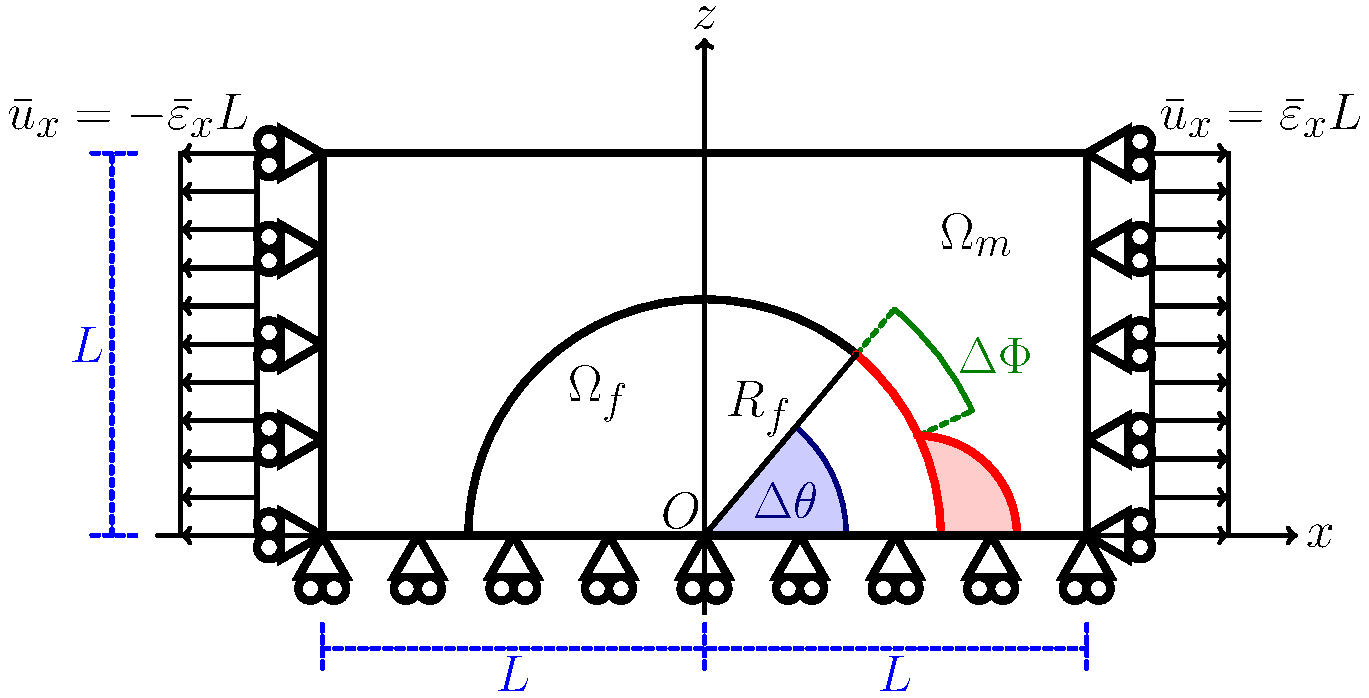
\includegraphics[width=\textwidth]{RUC.pdf}
\caption{Schematic of the model with its main parameters.}\label{fig:modelschem}
\end{figure}

As shown in Fig.~\ref{fig:modelschem}, the debond is placed symmetrically with respect to the $x$ axis and its size is characterized by the angle $\Delta\theta$ (which makes the full debond size equal to $2\Delta\theta$ and the full crack length equal to $R_{f}2{\Delta\theta}$). A region $\Delta\Phi$ of unknown size appears at the crack tip for large debond sizes (at least $\geq 60^{\circ}-80^{\circ}$), in which the crack faces are in contact with each other and free to slide. Frictionless contact is thus considered between the two crack faces to allow free sliding and avoid interpenetration. Symmetry with respect to the $x$ axis is applied on the lower boundary while the upper surface is left free. Kinematic coupling on the $x$-displacement is applied along the left and right sides of the model in the form of a constant $x$-displacement $\pm\bar{\varepsilon}_{x} L$, which corresponds to transverse strain $\bar{\varepsilon}_{x}$ equal to $1\%$ in the results here presented.

\begin{table}[!htbp]
 \centering
 \caption{Summary of the mechanical properties of fiber and matrix. $E$ stands for Young's modulus, $\mu$ for shear modulus and $\nu$ for Poisson's ratio.}
 \begin{tabular}{cccc}
\textbf{Material} & \textbf{$E\left[GPa\right]$}\ & \textbf{$\mu\left[GPa\right]$} & \textbf{$\nu\left[-\right]$} \\
\midrule
Glass fiber    & 70.0  & 29.2   & 0.2  \\
Epoxy    & 3.5    & 1.25   & 0.4
\end{tabular}
\label{tab:phaseprop}
\end{table}

The model problem is solved with the Finite Element Method (FEM) within the Abaqus environment, a commercial FEM software~\cite{abq12}. The model is meshed with second order, 2D, plane strain triangular (CPE6) and rectangular (CPE8) elements. A regular mesh of rectangular elements with almost unitary aspect ratio is used at the crack tip. The angular size $\delta$ of an element in the crack tip neighborhood represents the main parameter of the numerical analysis. The crack faces are modeled as element-based surfaces and a small-sliding contact pair interaction with no friction is imposed between them. The Mode I, Mode II and total Energy Release Rates (ERRs) (respectively referred to as $G_{I}$, $G_{II}$ and $G_{TOT}$) are evaluated using the VCCT~\cite{Krueger2004}, implemented in a in-house Python routine. A glass fiber-epoxy system is considered in the present work, and it is assumed that their response lies always in the linear elastic domain. The elastic properties of glass fiber and epoxy are reported in Table~\ref{tab:phaseprop}.

\section{Vectorial formulation of the Virtual Crack Closure Technique (VCCT)}
 
In order to express the VCCT formulation of the ERR in terms of FEM variables, we need to introduce a few rotation matrices in order to represent the discretized representation (FE mesh) of a crack along a circular interface. The position of the crack tip is characterized by the angular size of the crack (see Sec.~\ref{sec:femmodel} and Fig.~\ref{fig:modelschem} for reference) and the rotation corresponding to the crack tip reference frame is represented by the matrix $\underline{\underline{R}}_{\Delta\theta}$ defined as

\begin{equation}\label{eq:Rmatrix}
\underline{\underline{R}}_{\Delta\theta}=\begin{bmatrix}
\cos\left(\Delta\theta\right) & \sin\left(\Delta\theta\right) \\
-\sin\left(\Delta\theta\right) & \cos\left(\Delta\theta\right)
\end{bmatrix}.
\end{equation}

Nodes belonging to the elements sharing the crack tip are involved in the VCCT estimation of the ERR and it is assumed that, given a sufficiently fine discretization, they are aligned with the crack propagation direction defined at the crack tip. However, irrespectively of how small the elements in the crack tip neighborhood are, a misalignment always exists with respect to the assumed crack propagation direction (in the crack tip reference frame). This is measured by the matrices $\underline{\underline{P}}_{\delta}\left(p\right)$, defined as

\begin{equation}\label{eq:Pmatrix}
\underline{\underline{P}}_{\delta}\left(p\right)=\begin{bmatrix}
\cos\left(\left(1+\frac{1-p}{m}\right)\delta\right) & \sin\left(\left(1+\frac{1-p}{m}\right)\delta\right) \\
-\sin\left(\left(1+\frac{1-p}{m}\right)\delta\right) & \cos\left(\left(1+\frac{1-p}{m}\right)\delta\right)
\end{bmatrix}
\end{equation}

 and $\underline{\underline{Q}}_{\delta}\left(q\right)$, equal to 

\begin{equation}\label{eq:Qmatrix}
\underline{\underline{Q}}_{\delta}\left(q\right)=\begin{bmatrix}
\cos\left(\frac{q-1}{m}\delta\right) & \sin\left(\frac{q-1}{m}\delta\right) \\
-\sin\left(\frac{q-1}{m}\delta\right) & \cos\left(\frac{q-1}{m}\delta\right)
\end{bmatrix},
\end{equation}

respectively for the free and bonded nodes involved in the VCCT estimation. In Eqs.~\ref{eq:Pmatrix} and~\ref{eq:Qmatrix}, $\delta$ is the angular size of an element in the crack tip neighborhood (see Sec.~\ref{sec:femmodel} and Fig.~\ref{fig:modelschem}), $m$ is the order of the element shape functions and $p,q$ are indices referring to the nodes belonging respectively to free and bonded elements sharing the crack tip. Introducing the permutation matrix


\begin{equation}
\underline{\underline{P}}_{\pi}=\begin{bmatrix}
0 & 1\\
-1& 0
\end{bmatrix},
\end{equation}

it is possible to express the derivatives of rotation matrices $\underline{\underline{R}}_{\Delta\theta}$, $\underline{\underline{P}}_{\delta}$ and $\underline{\underline{Q}}_{\delta}$ with respect to their argument:

\begin{equation}\label{eq:rotmatdev}
\frac{\partial \underline{\underline{R}}_{\Delta\theta}}{\partial \Delta\theta}=\underline{\underline{D}}\cdot\underline{\underline{R}}_{\Delta\theta},\quad\frac{\partial \underline{\underline{P}}_{\delta}}{\partial \delta}=\left(1+\frac{1-p}{m}\right)\underline{\underline{D}}\cdot\underline{\underline{P}}_{\delta},\quad\frac{\partial \underline{\underline{Q}}_{\delta}}{\partial \delta}=\frac{q-1}{m}\underline{\underline{D}}\cdot\underline{\underline{Q}}_{\delta}.
\end{equation}

By means of Eqs.~\ref{eq:Pmatrix} and~\ref{eq:Qmatrix}, we can express the crack tip forces $
\underline{F}_{xy}=\begin{bmatrix}
F_{x} \\
F_{y}
\end{bmatrix}$ and crack displacements  $
\underline{u}_{xy}=\begin{bmatrix}
u_{x} \\
u_{y}
\end{bmatrix}$ in the crack tip reference frame (where the tangential direction $\theta$ correspond to the direction of crack propagation) while taking into account the misalignment to the finite  discretization as 

\begin{equation}\label{eq:FUrot}
\underline{F}_{r\theta}=\underline{\underline{Q}}_{\delta}\underline{\underline{R}}_{\Delta\theta}\underline{F}_{xy}\qquad\underline{u}_{r\theta}=\underline{\underline{P}}_{\delta}\underline{\underline{R}}_{\Delta\theta}\underline{u}_{xy}
\end{equation}

where $\underline{F}_{r\theta}=\begin{bmatrix}
F_{r} \\
F_{\theta}
\end{bmatrix}$ and $\underline{u}_{r\theta}=\begin{bmatrix}
u_{r} \\
u_{\theta}
\end{bmatrix}$.

The crack tip forces can be expressed as a function of the crack opening displacement as 

\begin{equation}\label{eq:ctforce1}
\underline{F}_{xy}=\underline{\underline{K}}_{xy}\underline{u}_{xy}+\underline{\widetilde{F}}_{xy},
\end{equation}
 
where $\underline{\underline{K}}_{xy}$ is in general a full matrix of the form $\underline{\underline{K}}_{xy}=\begin{bmatrix}
K_{xx}  K_{xy}\\
K_{yx}  K_{yy}
\end{bmatrix}$ and $\underline{\widetilde{F}}_{xy}$ represents the effect of the rest of the FE solution through the remaining nodes of the elements attached to the crack tip. As such, the term $\underline{\widetilde{F}}_{xy}$ can be expressed as a linear combination of the solution vector $\underline{u}_{N}$ of nodal displacements of the form $\underline{\underline{\widetilde{K}}}_{N}\underline{u}_{N}$. Equation~\ref{eq:ctforce1} thus become

\begin{equation}\label{eq:ctforce2}
\underline{F}_{xy}=\underline{\underline{K}}_{xy}\underline{u}_{xy}+\underline{\underline{\widetilde{K}}}_{N}\underline{u}_{N}.
\end{equation}

An exemplifying derivation of the relationships expressed in Equations~\ref{eq:ctforce1} and~\ref{eq:ctforce2} can be found in \ref{app:ctforcesexample}. It is worthwhile to observe that another author~\cite{Valvo2011} proposed a relationship of the form $\underline{F}_{xy}=\underline{\underline{K}}_{xy}\underline{u}_{xy}$. However, in~\cite{Valvo2011}, this relationship is assumed \emph{a priori} and manipulated to propose a revised version of the VCCT, based on the assumption that the matrix $\underline{\underline{K}}_{xy}$ should be diagonal to provide physically-consistent fracture mode partitioning. On the other hand, in the present work we derive the relationships of Eqs.~\ref{eq:ctforce1} and~\ref{eq:ctforce2} from the formulation of the Finite Element Method. According to our derivation, it seems correct that the matrix $\underline{\underline{K}}_{xy}$ should not in general be diagonal in order to take into account Poisson's effect. In fact, a positive crack opening displacement would cause a transverse displacement in the neighborhood of the crack tip. Given that material properties are different on the two sides of a bi-material interface, a net shear would be applied to the crack tip which would correspond to a net contribution to the crack tip force related to crack shear displacement. The analytical derivations presented in \ref{app:ctforcesexample} confirm these physical considerations.\\
Based upon the work of Raju~\cite{Raju1987}, we introduce the matrix $\underline{\underline{T}}_{pq}$ to represent the weights needed in the VCCT to account for the use of singular elements. As already done previously, indices $p$ and $q$ refer to nodes placed respectively on the free (crack face) and bonded side of the crack tip. Nodes are enumerated so that the crack tip has always index $1$, i.e. the higher the index the further the node is from the crack tip. Matrix $\underline{\underline{T}}_{pq}$ has always a size of $d\times d$, where $d=2$ for a $2D$ problem and $d=3$ for a $3D$ problem. An element $\underline{\underline{T}}_{pq}\left(i,j\right)$ with $i,j=1,\dots,d$ represents the weight to be assigned to the product of component $i$ of the displacement extracted at node $p$ with component $j$ of the force extracted at node $q$. The expression of $\underline{\underline{T}}_{pq}$ for quadrilateral elements with or without singularity is reported in \ref{app:Tpq}. Notice that, given $m$ is the order of the element shape functions, the element side has $m+1$ nodes and this represents the upper limit of indices $p$ and $q$.\\
By using matrix $\underline{\underline{T}}_{pq}$, it is possible to express the total ERR $G$ evaluated with the VCCT as

\begin{equation}\label{eq:gtot}
G_{TOT} = \frac{1}{2R_{f}\delta}\sum_{p=1}^{m+1}\sum_{q=1}^{m+1}Tr\left(\underline{u}_{r\theta,p}^{T}\underline{\underline{T}}_{pq}^{T}\underline{F}_{r\theta,q}\right).
\end{equation}

Introducing the vector $\underline{G}=\begin{bmatrix}
G_{I} \\
G_{II}
\end{bmatrix}$ of fracture mode ERRs, Mode I and Mode II ERR evaluated with the VCCT can be expressed as 

\begin{equation}\label{eq:g}
\underline{G} =\frac{1}{2R_{f}\delta}\sum_{p=1}^{m+1}\sum_{q=1}^{m+1}Diag\left(\underline{F}_{r\theta,q}\underline{u}_{r\theta,p}^{T}\underline{\underline{T}}_{pq}^{T}\right),
\end{equation}

where $Diag\left(\right)$ is the function that extracts the main diagonal of the input matrix as a column vector. Substituting Equations~\ref{eq:FUrot} and~\ref{eq:ctforce2} in Equations~\ref{eq:gtot} and~\ref{eq:g}, we can express the Mode I, Mode II and total Energy Release Rate as a function of the crack displacements and the FE solution (more details in \ref{app:ctforcesexample}) as 

\begin{equation}\label{eq:gtotlong}
\begin{split}
G_{TOT} =&\frac{1}{2R_{f}\delta}\sum_{p=1}^{m+1}\sum_{q=1}^{m+1}Tr\left(\underline{\underline{Q}}_{\delta}\underline{\underline{R}}_{\Delta\theta}\underline{\underline{K}}_{xy,q}\underline{u}_{xy,q}\underline{u}_{xy,p}^{T}\underline{\underline{R}}_{\Delta\theta}^{T}\underline{\underline{P}}_{\delta}^{T}\underline{\underline{T}}_{pq}^{T}\right)+\\&+\frac{1}{2R_{f}\delta}\sum_{p=1}^{m+1}\sum_{q=1}^{m+1}Tr\left(\underline{\underline{Q}}_{\delta}\underline{\underline{R}}_{\Delta\theta}\underline{\widetilde{F}}_{xy,q}\underline{u}_{xy,p}^{T}\underline{\underline{R}}_{\Delta\theta}^{T}\underline{\underline{P}}_{\delta}^{T}\underline{\underline{T}}_{pq}^{T}\right)
\end{split}
\end{equation}

and

\begin{equation}
\begin{split}
\underline{G}=\begin{bmatrix}
G_{I} \\
G_{II}
\end{bmatrix}=&\frac{1}{2R_{f}\delta}\sum_{p=1}^{m+1}\sum_{q=1}^{m+1}Diag\left(\underline{\underline{Q}}_{\delta}\underline{\underline{R}}_{\Delta\theta}\underline{\underline{K}}_{xy,q}\underline{u}_{xy,q}\underline{u}_{xy,p}^{T}\underline{\underline{R}}_{\Delta\theta}^{T}\underline{\underline{P}}_{\delta}^{T}\underline{\underline{T}}_{pq}^{T}\right)+\\
&+\frac{1}{2R_{f}\delta}\sum_{p=1}^{m+1}\sum_{q=1}^{m+1}Diag\left(\underline{\underline{Q}}_{\delta}\underline{\underline{R}}_{\Delta\theta}\underline{\underline{\widetilde{K}}}_{N,q}\underline{u}_{N}\underline{u}_{xy,p}^{T}\underline{\underline{R}}_{\Delta\theta}^{T}\underline{\underline{P}}_{\delta}^{T}\underline{\underline{T}}_{pq}^{T}\right)
\end{split}
\end{equation}

\section{Rotational invariance of $G_{TOT}$}

Recalling Equation~\ref{eq:gtotlong} and observing that matrix $\underline{\underline{T}}_{pq}$ is always equal to the identity matrix pre-multiplied by a suitable real constant (see Eq.~\ref{eq:Tpq} in \ref{app:Tpq}), the total Energy Release Rate can be rewritten as

\begin{equation}\label{eq:gtotlong1}
\begin{split}
G_{TOT}&=\frac{1}{2R_{f}\delta}\sum_{p=1}^{m+1}\sum_{q=1}^{m+1}Tr\left(\underline{\underline{Q}}_{\delta}\underline{\underline{R}}_{\Delta\theta}\left(\underline{\underline{K}}_{xy,q}\underline{u}_{xy,q}+\underline{\widetilde{F}}_{xy,q}\right)\underline{u}_{xy,p}^{T}\underline{\underline{T}}_{pq}^{T}\underline{\underline{R}}_{\Delta\theta}^{T}\underline{\underline{P}}_{\delta}^{T}\right)=\\
&=\frac{1}{2R_{f}\delta}\sum_{p=1}^{m+1}\sum_{q=1}^{m+1}Tr\left(\underline{\underline{Q}}_{\delta}\underline{\underline{R}}_{\Delta\theta}\underline{F}_{xy,q}\underline{u}_{xy,p}^{T}\underline{\underline{T}}_{pq}^{T}\underline{\underline{R}}_{\Delta\theta}^{T}\underline{\underline{P}}_{\delta}^{T}\right),
\end{split}
\end{equation}

where $\underline{F}_{xy}$ and $\underline{u}_{xy}$ are the vectors of respectively the crack tip forces and crack displacements in the global ($x-y$) reference frame. Given that $\underline{\underline{Q}}_{\delta}$, $\underline{\underline{P}}_{\delta}$ and $\underline{\underline{R}}_{\Delta\theta}$ all represent a linear transformation (a rigid rotation in particular), the invariance of the trace to linear transformations ensures that

\begin{equation}\label{eq:gtotlong2}
\begin{split}
G_{TOT}&=\frac{1}{2R_{f}\delta}\sum_{p=1}^{m+1}\sum_{q=1}^{m+1}Tr\left(\underline{\underline{Q}}_{\delta}\underline{\underline{R}}_{\Delta\theta}\underline{F}_{xy,q}\underline{u}_{xy,p}^{T}\underline{\underline{T}}_{pq}^{T}\underline{\underline{R}}_{\Delta\theta}^{T}\underline{\underline{P}}_{\delta}^{T}\right)=\\
&=\frac{1}{2R_{f}\delta}\sum_{p=1}^{m+1}\sum_{q=1}^{m+1}Tr\left(\underline{F}_{xy,q}\underline{u}_{xy,p}^{T}\underline{\underline{T}}_{pq}^{T}\right).
\end{split}
\end{equation}

As $G_{TOT}$ was defined according to Equation~\ref{eq:gtot} and given that $Tr\left(AB\right)=Tr\left(BA\right)$, it holds that 

\begin{equation}\label{eq:gtotrotinv}
\begin{split}
G_{TOT} &= \frac{1}{2R_{f}\delta}\sum_{p=1}^{m+1}\sum_{q=1}^{m+1}\underline{u}_{r\theta,p}^{T}\underline{\underline{T}}_{pq}^{T}\underline{F}_{r\theta,q}=\frac{1}{2R_{f}\delta}\sum_{p=1}^{m+1}\sum_{q=1}^{m+1}Tr\left(\underline{F}_{r\theta,q}\underline{u}_{r\theta,p}^{T}\underline{\underline{T}}_{pq}^{T}\right)=\\
&=\frac{1}{2R_{f}\delta}\sum_{p=1}^{m+1}\sum_{q=1}^{m+1}Tr\left(\underline{F}_{xy,q}\underline{u}_{xy,p}^{T}\underline{\underline{T}}_{pq}^{T}\right)=\frac{1}{2R_{f}\delta}\sum_{p=1}^{m+1}\sum_{q=1}^{m+1}\underline{u}_{xy,p}^{T}\underline{\underline{T}}_{pq}^{T}\underline{F}_{xy,q}
\end{split}
\end{equation}

which shows that the total Energy Release Rate is invariant to rigid rotations and can be calculated equivalently with forces and displacements expressed in the local crack tip reference frame or the global reference frame. The analytical result is confirmed by the numerical solution of the fiber-matrix interface crack with different element orders and model fiber volume fractions, as shown in Figure~\ref{fig:gtotrotinvnum}.

\begin{figure}[!h]
\centering
    \begin{subfigure}[b]{0.48\textwidth}
        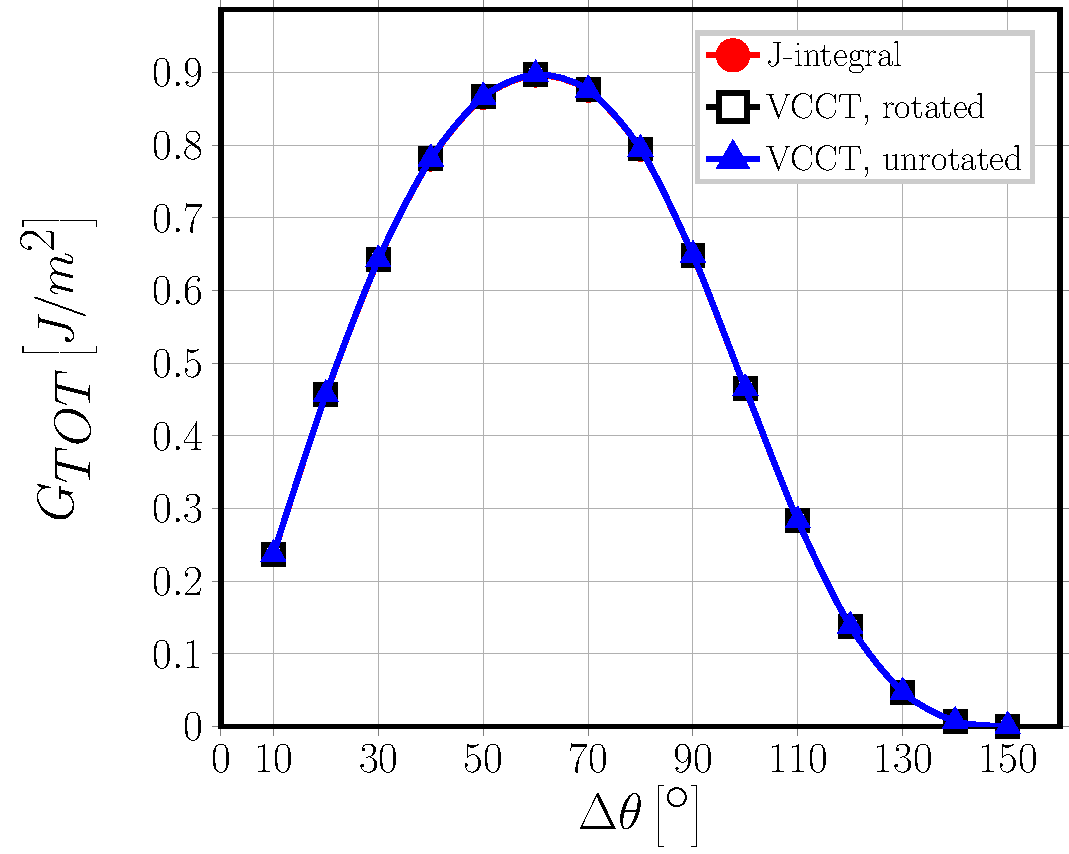
\includegraphics[width=\textwidth]{Vf0_1-free-1st-05-invrot-GTOT.pdf}
       \caption{$V_{f}=0.1\%$, $1^{st}$ order elements, $\delta=0.05^{\circ}$.}
    \end{subfigure}
    ~
    \begin{subfigure}[b]{0.48\textwidth}
        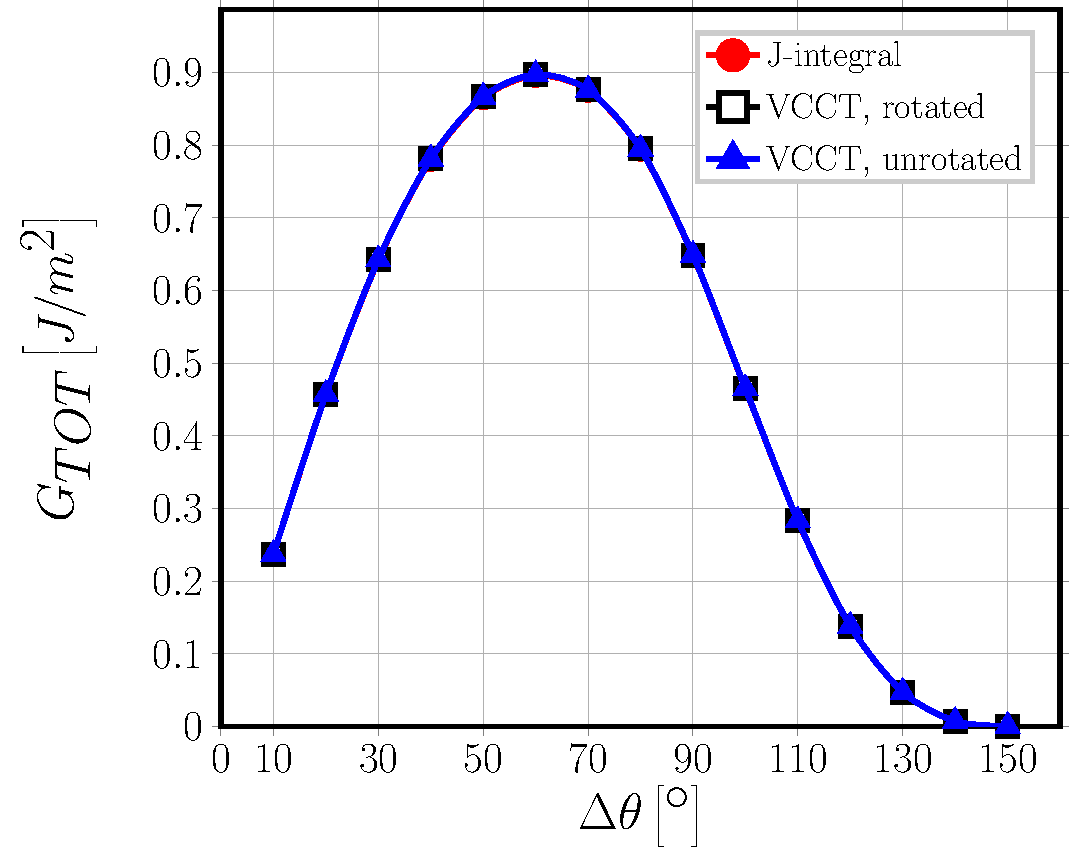
\includegraphics[width=\textwidth]{Vf0_1-free-2nd-05-invrot-GTOT.pdf}
       \caption{$V_{f}=0.1\%$, $2^{nd}$ order elements, $\delta=0.05^{\circ}$.}
    \end{subfigure}

    \begin{subfigure}[b]{0.48\textwidth}
        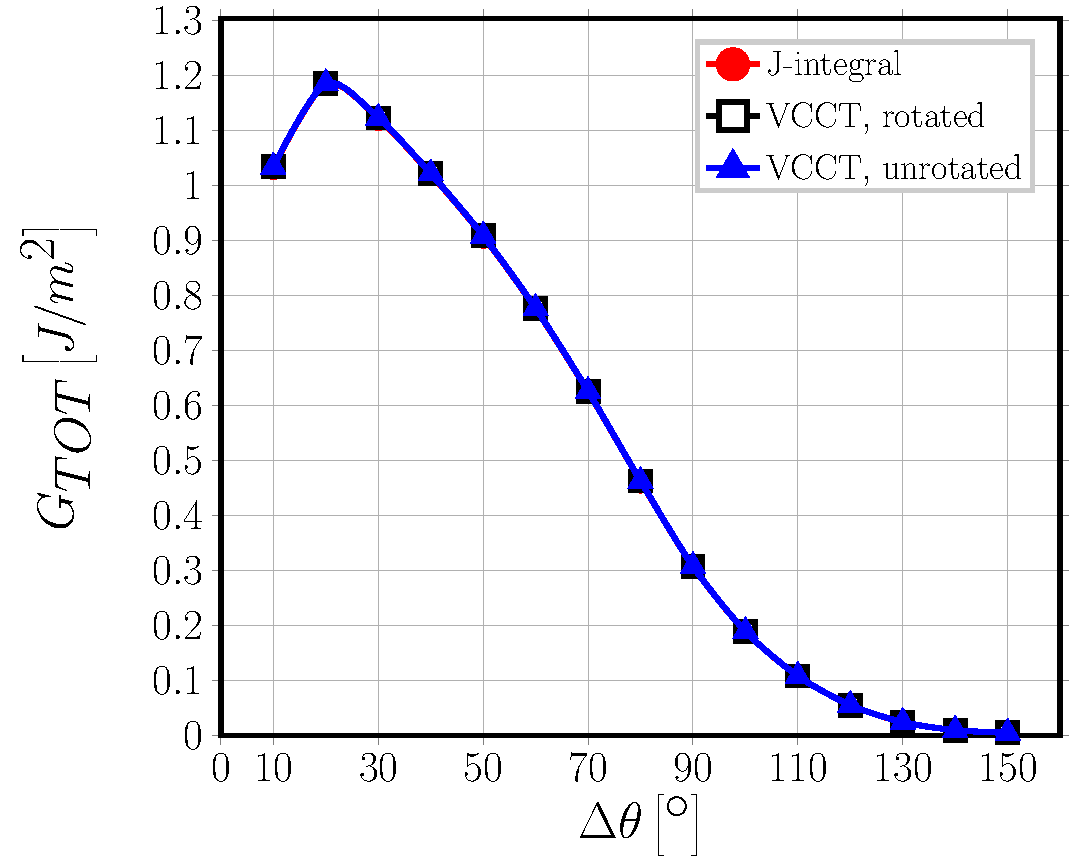
\includegraphics[width=\textwidth]{Vf40-free-1st-05-invrot-GTOT.pdf}
       \caption{$V_{f}=40\%$, $1^{st}$ order elements, $\delta=0.05^{\circ}$.}
    \end{subfigure}
    ~
    \begin{subfigure}[b]{0.48\textwidth}
        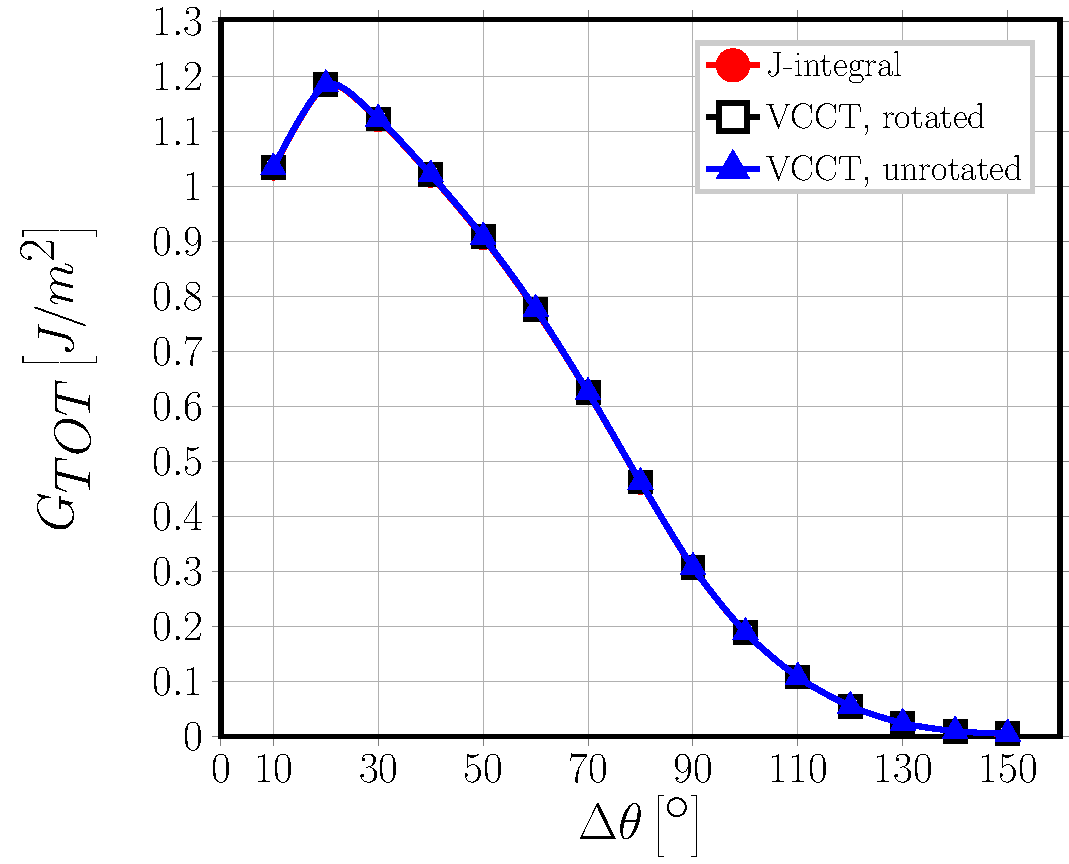
\includegraphics[width=\textwidth]{Vf40-free-2nd-05-invrot-GTOT.pdf}
       \caption{$V_{f}=40\%$, $2^{nd}$ order elements, $\delta=0.05^{\circ}$ .}
    \end{subfigure}

\caption{Numerical invariance of the total Energy Release Rate: $G_{TOT}$ computed with the VCCT with rotated forces and displacements (label \emph{rotated}), with the VCCT with forces and displacements in the global reference frame (label \emph{unrotated}) and with J-integral method (label \emph{J-integral}).}\label{fig:gtotrotinvnum}
\end{figure}

The result of Equation~\ref{eq:gtotrotinv} has also physical implications:

\begin{itemize}[\label={--}]
\item given that stress and displacement fields at the crack tip are the same, two cracks with different crack paths are energetically equivalent with respect to the total Energy Release Rate;
\item given that laws of the type $G_{TOT}\geq G_{c}$ govern crack propagation, if $G_{c}$ do not depend on mode ratio, crack orientation will not affect its growth.
\end{itemize}

\section{Convergence analysis}

\subsection{Analytical considerations}

Substituting Equations~\ref{eq:rotmatdev} in the derivative of Equation~\ref{eq:g}, we can investigate the dependency of Mode I and Mode II ERR with respect to the size $\delta$ of an element in the crack tip neighborhood through 

\begin{equation}
\scriptsize
\begin{split}
\frac{\partial \underline{G}}{\partial \delta}=&-\frac{1}{2R_{f}\delta^{2}}\sum_{p=1}^{m+1}\sum_{q=1}^{m+1}Diag\left(\underline{\underline{Q}}_{\delta}\underline{\underline{R}}_{\Delta\theta}\underline{\underline{K}}_{xy}\underline{u}_{xy}\underline{u}_{xy}^{T}\underline{\underline{R}}_{\Delta\theta}^{T}\underline{\underline{P}}_{\delta}^{T}\underline{\underline{T}}_{pq}^{T}\right)-\frac{1}{2R_{f}\delta^{2}}\sum_{p=1}^{m+1}\sum_{q=1}^{m+1}Diag\left(\underline{\underline{Q}}_{\delta}\underline{\underline{R}}_{\Delta\theta}\underline{\underline{\widetilde{K}}}_{N}\underline{u}_{N}\underline{u}_{xy}^{T}\underline{\underline{R}}_{\Delta\theta}^{T}\underline{\underline{P}}_{\delta}^{T}\underline{\underline{T}}_{pq}^{T}\right)+\\
+&\frac{1}{2R_{f}\delta}\sum_{p=1}^{m+1}\sum_{q=1}^{m+1}Diag\left(\underline{\underline{Q}}_{\delta}\underline{\underline{R}}_{\Delta\theta}\underline{\underline{K}}_{xy}\underline{u}_{xy}\underline{u}_{xy}^{T}\underline{\underline{R}}_{\Delta\theta}^{T}\underline{\underline{P}}_{\delta}^{T}\underline{\underline{D}}^{T}\underline{\underline{T}}_{pq}^{T}\right)+\frac{1}{2R_{f}\delta}\sum_{p=1}^{m+1}\sum_{q=1}^{m+1}Diag\left(\underline{\underline{Q}}_{\delta}\underline{\underline{R}}_{\Delta\theta}\underline{\underline{\widetilde{K}}}_{N}\underline{u}_{N}\underline{u}_{xy}^{T}\underline{\underline{R}}_{\Delta\theta}^{T}\underline{\underline{P}}_{\delta}^{T}\underline{\underline{D}}^{T}\underline{\underline{T}}_{pq}^{T}\right)+\\
+&\frac{1}{2R_{f}\delta}\sum_{p=1}^{m+1}\sum_{q=1}^{m+1}Diag\left(\underline{\underline{D}}\underline{\underline{Q}}_{\delta}\underline{\underline{R}}_{\Delta\theta}\underline{\underline{K}}_{xy}\underline{u}_{xy}\underline{u}_{xy}^{T}\underline{\underline{R}}_{\Delta\theta}^{T}\underline{\underline{P}}_{\delta}^{T}\underline{\underline{T}}_{pq}^{T}\right)+\frac{1}{2R_{f}\delta}\sum_{p=1}^{m+1}\sum_{q=1}^{m+1}Diag\left(\underline{\underline{D}}\underline{\underline{Q}}_{\delta}\underline{\underline{R}}_{\Delta\theta}\underline{\underline{\widetilde{K}}}_{N}\underline{u}_{N}\underline{u}_{xy}^{T}\underline{\underline{R}}_{\Delta\theta}^{T}\underline{\underline{P}}_{\delta}^{T}\underline{\underline{T}}_{pq}^{T}\right)+\\
+&\frac{1}{2R_{f}\delta}\sum_{p=1}^{m+1}\sum_{q=1}^{m+1}Diag\left(\underline{\underline{Q}}_{\delta}\underline{\underline{R}}_{\Delta\theta}\underline{\underline{K}}_{xy}\frac{\partial \underline{u}_{xy}}{\partial \delta}\underline{u}_{xy}^{T}\underline{\underline{R}}_{\Delta\theta}^{T}\underline{\underline{P}}_{\delta}^{T}\underline{\underline{T}}_{pq}^{T}\right)+\frac{1}{2R_{f}\delta}\sum_{p=1}^{m+1}\sum_{q=1}^{m+1}Diag\left(\underline{\underline{Q}}_{\delta}\underline{\underline{R}}_{\Delta\theta}\underline{\underline{\widetilde{K}}}_{N}\frac{\partial \underline{u}_{N}}{\partial \delta}\underline{u}_{xy}^{T}\underline{\underline{R}}_{\Delta\theta}^{T}\underline{\underline{P}}_{\delta}^{T}\underline{\underline{T}}_{pq}^{T}\right)+\\
+&\frac{1}{2R_{f}\delta}\sum_{p=1}^{m+1}\sum_{q=1}^{m+1}Diag\left(\underline{\underline{Q}}_{\delta}\underline{\underline{R}}_{\Delta\theta}\underline{\underline{K}}_{xy}\underline{u}_{xy}\frac{\partial \underline{u}_{xy}^{T}}{\partial \delta}\underline{\underline{R}}_{\Delta\theta}^{T}\underline{\underline{P}}_{\delta}^{T}\underline{\underline{T}}_{pq}^{T}\right)+\frac{1}{2R_{f}\delta}\sum_{p=1}^{m+1}\sum_{q=1}^{m+1}Diag\left(\underline{\underline{Q}}_{\delta}\underline{\underline{R}}_{\Delta\theta}\underline{\underline{\widetilde{K}}}_{N}\underline{u}_{N}\frac{\partial \underline{u}_{xy}^{T}}{\partial \delta}\underline{\underline{R}}_{\Delta\theta}^{T}\underline{\underline{P}}_{\delta}^{T}\underline{\underline{T}}_{pq}^{T}\right);
\end{split}
\end{equation}

which, after refactoring, provides

\begin{equation}\label{eq:Gdev}
\scriptsize
\begin{split}
\frac{\partial \underline{G}}{\partial \delta}=&\frac{1}{\delta}\underline{G}+\frac{1}{2R_{f}\delta}\sum_{p=1}^{m+1}\sum_{q=1}^{m+1}Diag\left(\underline{\underline{Q}}_{\delta}\underline{\underline{R}}_{\Delta\theta}\left(\underline{\underline{K}}_{xy}\underline{u}_{xy}+\underline{\underline{\widetilde{K}}}_{N}\underline{u}_{N}\right)\underline{u}_{xy}^{T}\underline{\underline{R}}_{\Delta\theta}^{T}\underline{\underline{P}}_{\delta}^{T}\underline{\underline{D}}^{T}\underline{\underline{T}}_{pq}^{T}\right)+\\
+&\frac{1}{2R_{f}\delta}\sum_{p=1}^{m+1}\sum_{q=1}^{m+1}Diag\left(\underline{\underline{D}}\underline{\underline{Q}}_{\delta}\underline{\underline{R}}_{\Delta\theta}\left(\underline{\underline{K}}_{xy}\underline{u}_{xy}+\underline{\underline{\widetilde{K}}}_{N}\underline{u}_{N}\right)\underline{u}_{xy}^{T}\underline{\underline{R}}_{\Delta\theta}^{T}\underline{\underline{P}}_{\delta}^{T}\underline{\underline{T}}_{pq}^{T}\right)+\\
+&\frac{1}{R_{f}\delta}\sum_{p=1}^{m+1}\sum_{q=1}^{m+1}Diag\left(\underline{\underline{Q}}_{\delta}\underline{\underline{R}}_{\Delta\theta}\underline{\underline{K}}_{xy}\frac{\partial \underline{u}_{xy}}{\partial \delta}\underline{u}_{xy}^{T}\underline{\underline{R}}_{\Delta\theta}^{T}\underline{\underline{P}}_{\delta}^{T}\underline{\underline{T}}_{pq}^{T}\right)+\frac{1}{2R_{f}\delta}\sum_{p=1}^{m+1}\sum_{q=1}^{m+1}Diag\left(\underline{\underline{Q}}_{\delta}\underline{\underline{R}}_{\Delta\theta}\underline{\underline{\widetilde{K}}}_{N}\frac{\partial \underline{u}_{N}}{\partial \delta}\underline{u}_{xy}^{T}\underline{\underline{R}}_{\Delta\theta}^{T}\underline{\underline{P}}_{\delta}^{T}\underline{\underline{T}}_{pq}^{T}\right)+\\
+&\frac{1}{2R_{f}\delta}\sum_{p=1}^{m+1}\sum_{q=1}^{m+1}Diag\left(\underline{\underline{Q}}_{\delta}\underline{\underline{R}}_{\Delta\theta}\underline{\underline{\widetilde{K}}}_{N}\underline{u}_{N}\frac{\partial \underline{u}_{xy}^{T}}{\partial \delta}\underline{\underline{R}}_{\Delta\theta}^{T}\underline{\underline{P}}_{\delta}^{T}\underline{\underline{T}}_{pq}^{T}\right).
\end{split}
\end{equation}

Following the asymptotic analysis of~\cite{Williams1959,Comninou1990}, in the case of an \emph{open crack} the displacement in the crack tip neighborhood will have a functional form of the type

\begin{equation}\label{eq:basicasymptotic}
u\left(\delta\right)\sim \sqrt{\delta}\left(\sin,\cos\right)\left(\epsilon\log{\delta}\right)\quad\text{with}\quad\epsilon=\frac{1}{2\pi}\log{\left(\frac{1-\beta}{1+\beta}\right)}
\end{equation}

and $\beta$ is Dundurs' parameter introduced in Section~\ref{sec:intro}. Application of Equation~\ref{eq:basicasymptotic} to the terms on the right hand side of Eq.~\ref{eq:Gdev} provides:

\begin{equation}\label{eq:asym1}
\underline{u}_{xy},\underline{u}_{N}\sim u\left(\delta\right)\sim\sqrt{\delta}\left(\sin,\cos\right)\left(\epsilon\log{\delta}\right)\xrightarrow{\delta\rightarrow 0}0;
\end{equation}

\begin{equation}\label{eq:asym2}
\underline{u}_{xy}\underline{u}_{xy}^{T},\underline{u}_{N}\underline{u}_{xy}^{T}\sim u^{2}\left(\delta\right)\sim\delta\left(\sin^{2},\cos^{2},\sin\cdot\cos\right)\left(\epsilon\log{\delta}\right)\xrightarrow{\delta\rightarrow 0}0;
\end{equation}

\begin{equation}\label{eq:asym3}
\frac{\partial \underline{u}_{xy}}{\partial \delta}\underline{u}_{xy}^{T},\frac{\partial \underline{u}_{N}}{\partial \delta}\underline{u}_{xy}^{T}\sim -\frac{1}{2}\left(\sin^{2},\cos^{2},\sin\cdot\cos\right)\left(\epsilon\log{\delta}\right)+\left(-\sin^{2},\cos^{2},\pm\sin\cdot\cos\right)\left(\epsilon\log{\delta}\right)\xrightarrow{\delta\rightarrow 0}finite;
\end{equation}

\begin{equation}\label{eq:asym4}
\underline{G}\sim\frac{1}{\delta}\underline{u}_{xy}\underline{u}_{xy}^{T}\sim \frac{1}{\delta}u^{2}\left(\delta\right)\sim\left(\sin^{2},\cos^{2},\sin\cdot\cos\right)\left(\epsilon\log{\delta}\right)\xrightarrow{\delta\rightarrow 0}finite.
\end{equation}

In Equations~\ref{eq:asym1}-\ref{eq:asym4}, the multiplication by a trigonometric function of the type $\left(\sin,\cos,\sin^{2},\cos^{2},\sin\cdot\cos\right)$ prevents the divergence of the asymptote. Recalling Eqs.~\ref{eq:Pmatrix} and~\ref{eq:Qmatrix}, in the limit of $\delta\rightarrow 0$ the rotation matrices become equal to the identity matrix:

\begin{equation}\label{eq:PQasym}
\underline{\underline{P}}_{\delta},\underline{\underline{Q}}_{\delta}\xrightarrow{\delta\rightarrow 0}\begin{bmatrix}1&0\\0&1\end{bmatrix}.
\end{equation}

Applying the results of Equations~\ref{eq:asym1}-\ref{eq:PQasym} to Eq.~\ref{eq:Gdev}, it can be shown that the derivative of $\underline{G}$ can be split in a factor that goes to $0$ in the limit of $\delta\rightarrow 0$ and in a factor independent of $\delta$:

\begin{equation}
\lim_{\delta\rightarrow 0}\frac{\partial \underline{G}}{\partial \delta}\sim\frac{1}{\delta}\left(\cancelto{0}{\underline{F}\left(\delta\right)}+\underline{C}\right).
\end{equation}

Thus, asymptotically, the Mode I and Mode II Energy Release Rate behave like the logarithm of the angular size $\delta$ of the elements in the crack tip neighborhood:

\begin{equation}
\lim_{\delta\rightarrow 0}\frac{\partial \underline{G}}{\partial \delta}\sim\frac{1}{\delta}\quad\xrightarrow{\int d\delta}\quad\lim_{\delta\rightarrow 0}\underline{G}\sim \underline{A}\log(\delta)+\underline{B}.
\end{equation}

\subsection{Numerical results}

Evaluations of the Mode I, Mode II and total Energy Release Rate using the VCCT applied to the FE solution of the fiber-matrix interface crack in the single fiber model of Sec.~\ref{sec:femmodel} are reported respectively in Fig.~\ref{fig:ginum}, Fig.~\ref{fig:giinum} and Fig.~\ref{fig:gtotnum}.

\begin{figure}[!h]
\centering
    \begin{subfigure}[b]{0.48\textwidth}
        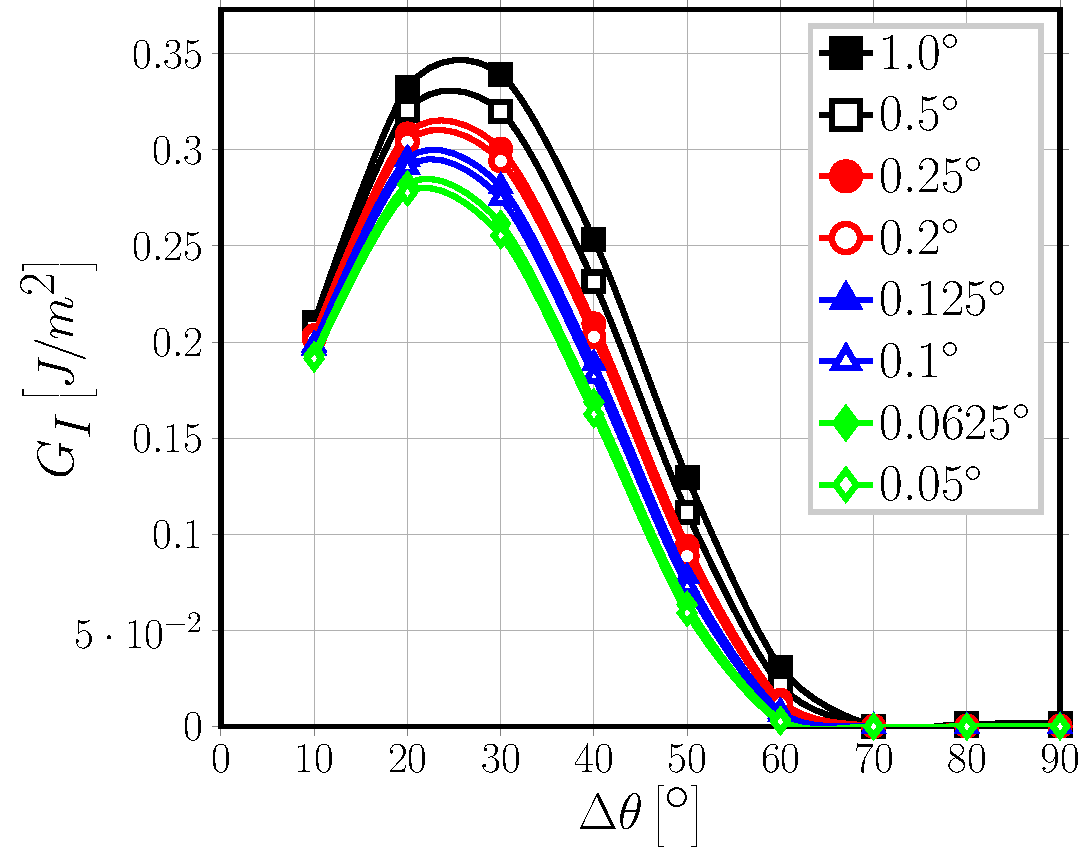
\includegraphics[width=\textwidth]{Vf0_1-free-1st-GI.pdf}
       \caption{$V_{f}=0.1\%$, $1^{st}$ order elements.}
    \end{subfigure}
    ~
    \begin{subfigure}[b]{0.48\textwidth}
        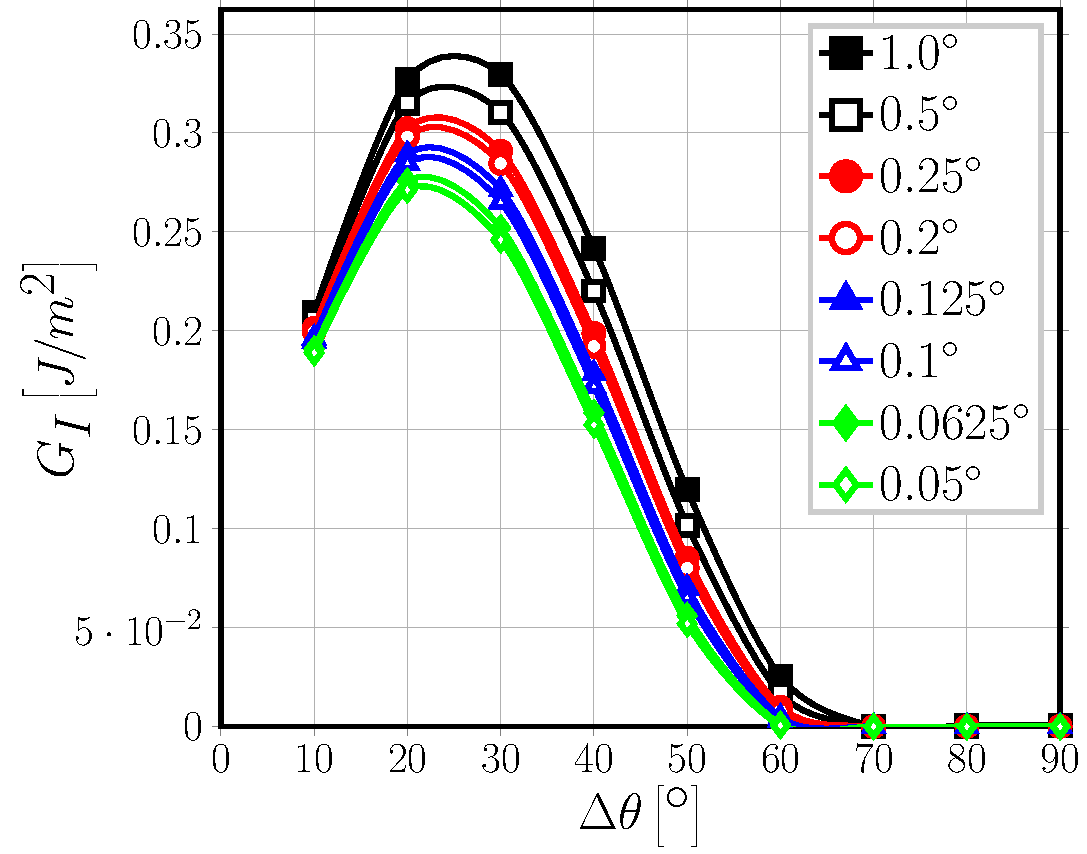
\includegraphics[width=\textwidth]{Vf0_1-free-2nd-GI.pdf}
       \caption{$V_{f}=0.1\%$, $2^{nd}$ order elements.}
    \end{subfigure}

    \begin{subfigure}[b]{0.48\textwidth}
        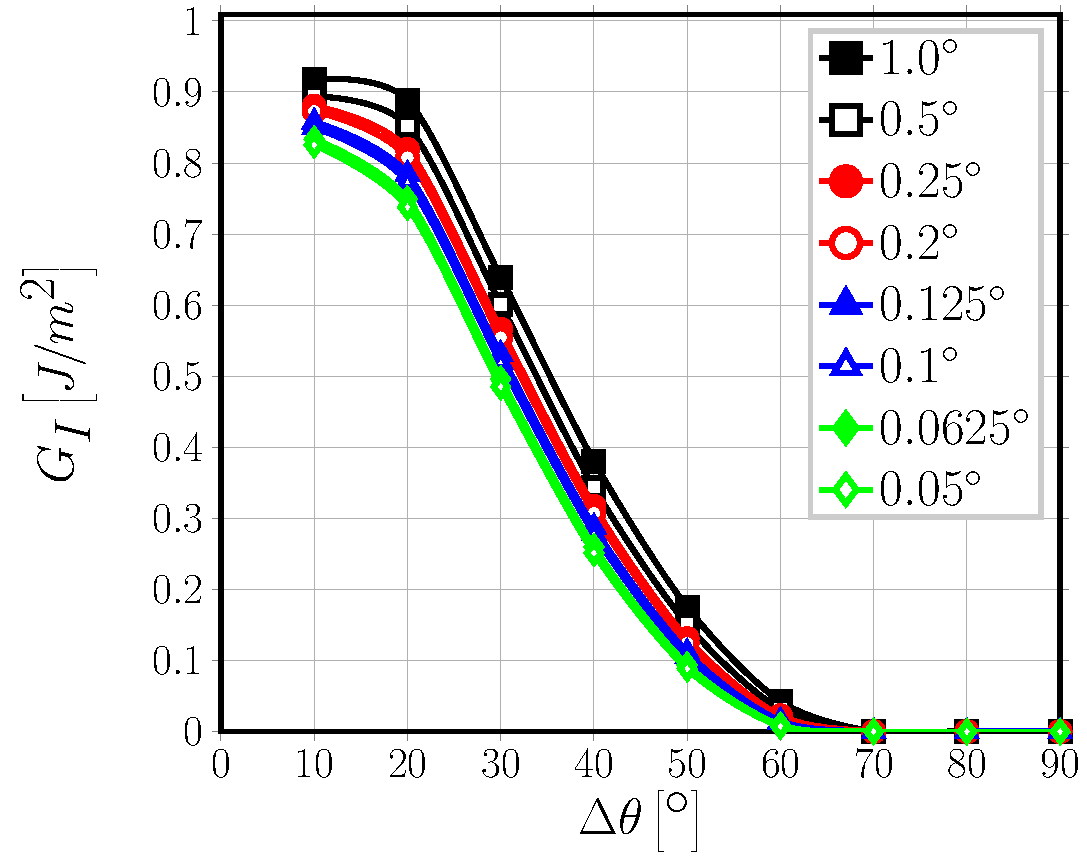
\includegraphics[width=\textwidth]{Vf40-free-1st-GI.pdf}
       \caption{$V_{f}=40\%$, $1^{st}$ order elements.}
    \end{subfigure}
    ~
    \begin{subfigure}[b]{0.48\textwidth}
        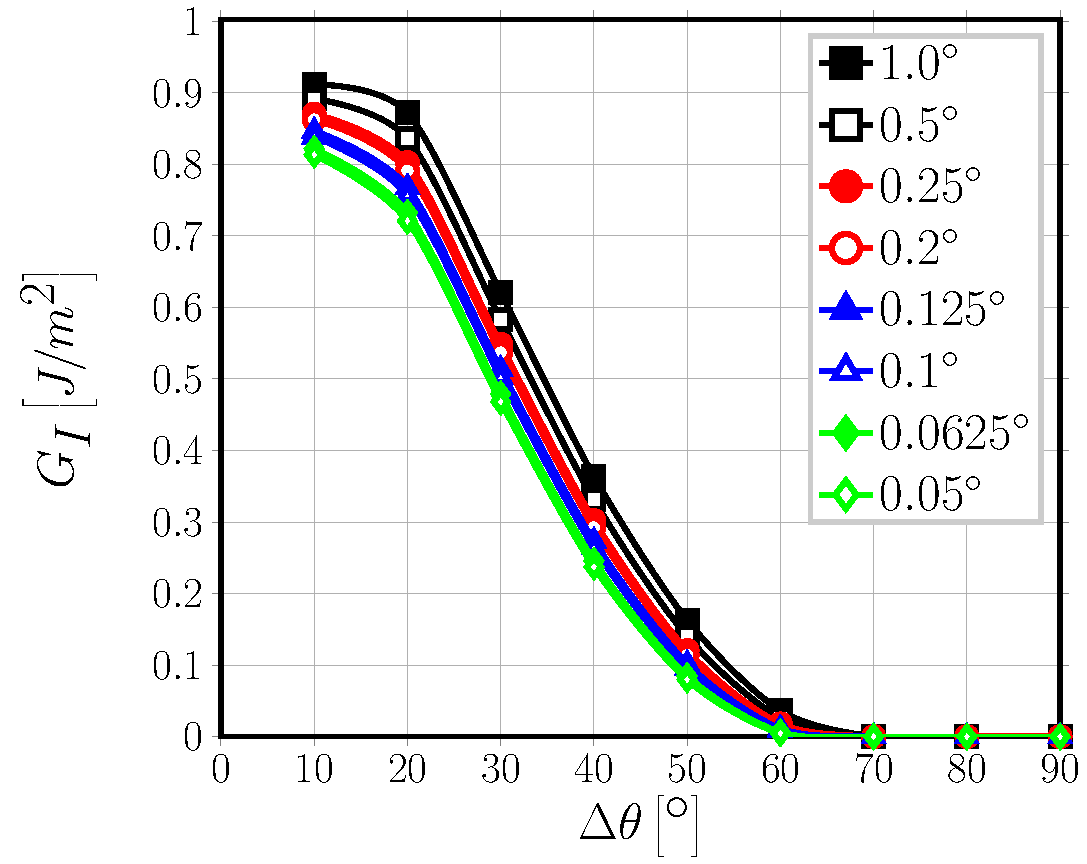
\includegraphics[width=\textwidth]{Vf40-free-2nd-GI.pdf}
       \caption{$V_{f}=40\%$, $2^{nd}$ order elements.}
    \end{subfigure}

\caption{Effect of the size $\delta$ of an element at the crack tip on Mode I ERR.}\label{fig:ginum}
\end{figure}

Results for Mode I ERR in Fig.~\ref{fig:ginum} show clearly the transition from the \emph{open} crack regime, where Mode I ERR is different from zero, to the \emph{closed} crack regime of the debond, where $G_{I}=0$. Looking at Fig.~\ref{fig:ginum}, the crack is \emph{open} for $\Delta\theta\leq60^{\circ}$ and it is \emph{closed}, i.e. a contact zone is present, for $\Delta\theta\geq70^{\circ}$. As expected from the analysis of the previous section, and given that Mode I ERR is different from zero only in the \emph{open} crack regime, a significant dependence on the element size $\delta$ can be observed in  Fig.~\ref{fig:ginum} when using both $1^{st}$ and $2^{nd}$ order elements and with both an effectively infinite ($V_{f}=0.1\%$) and finite size ($V_{f}=40\%$) matrix. At first sight, it is immediate to see from Fig.~\ref{fig:ginum} that a decrease in $\delta$ leads to a decrease in $G_{I}$. However, two further effects can be observed due to the refinement of the mesh at the crack tip, i.e. the decrease of the element size $\delta$. First, the occurrence of the peak $G_{I}$ is shifted to lower angles for very low volume fractions: it occurs at $\Delta\theta=30^{\circ}$ with $\delta=1.0^{\circ}, 0.5^{\circ}$ and at $\Delta\theta=20^{\circ}$ with $\delta\leq0.25^{\circ}$ for both $1^{st}$ and $2^{nd}$ order elements and $V_{f}=0.1\%$. Second, the apperance of the contact zone, i.e. the switch to the \emph{closed} crack regime, is anticipated to smaller debonds: it occurs at  $\Delta\theta=70^{\circ}$ with $\delta\geq0.2^{\circ}$ and at $\Delta\theta=60^{\circ}$ with $\delta<0.2^{\circ}$ for both $1^{st}$ and $2^{nd}$ order elements and both $V_{f}=0.1\%$ and $V_{f}=40\%$.

\begin{figure}[!h]
\centering
    \begin{subfigure}[b]{0.48\textwidth}
        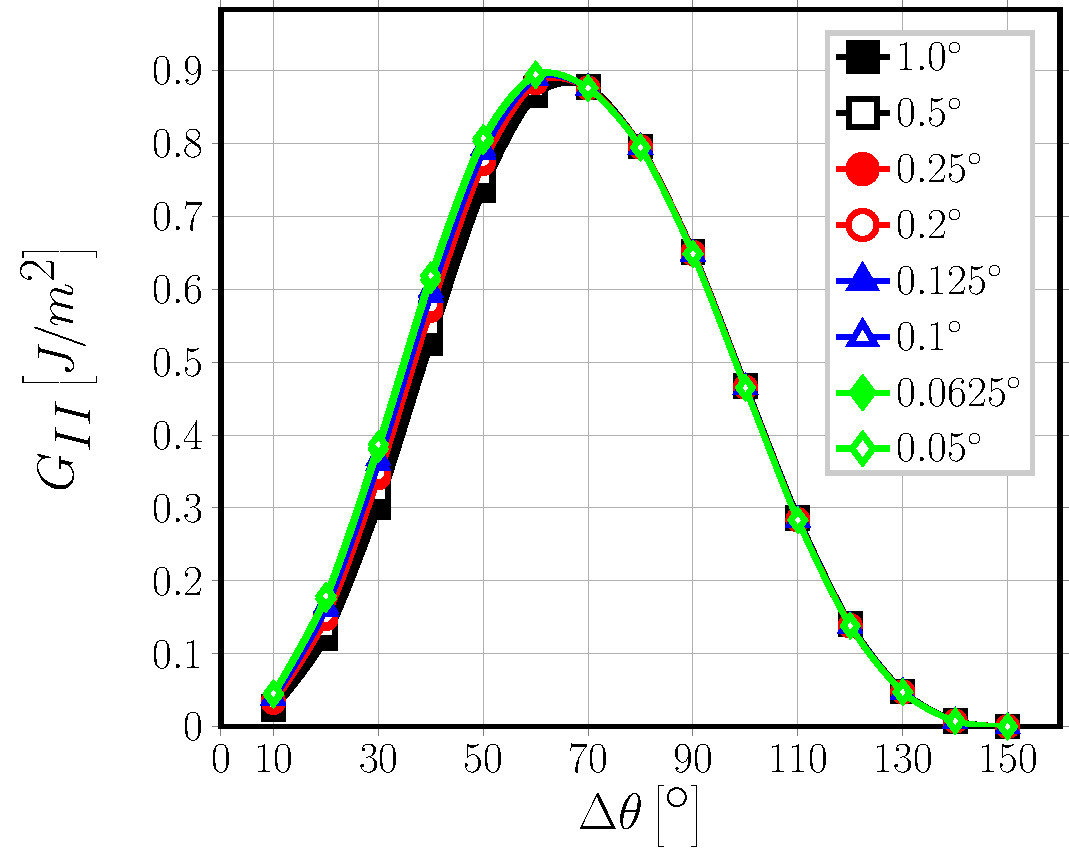
\includegraphics[width=\textwidth]{Vf0_1-free-1st-GII.pdf}
       \caption{$V_{f}=0.1\%$, $1^{st}$ order elements.}
    \end{subfigure}
    ~
    \begin{subfigure}[b]{0.48\textwidth}
        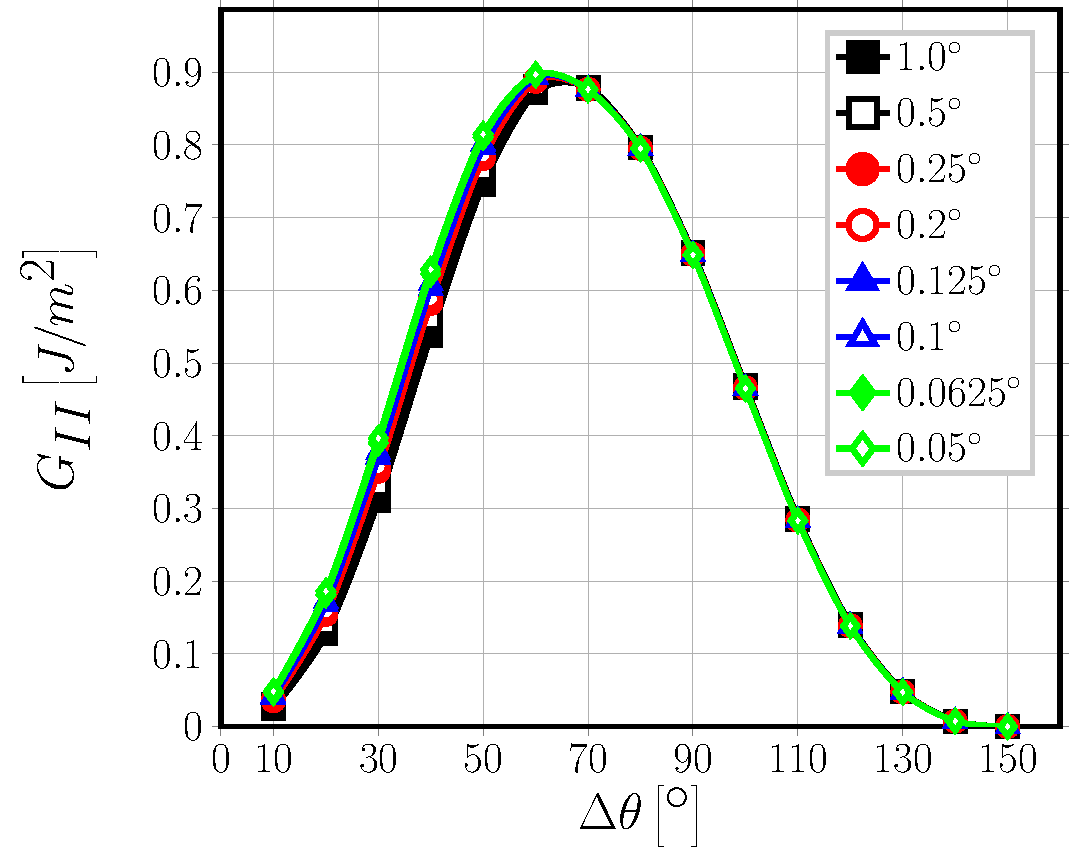
\includegraphics[width=\textwidth]{Vf0_1-free-2nd-GII.pdf}
       \caption{$V_{f}=0.1\%$, $2^{nd}$ order elements.}
    \end{subfigure}

    \begin{subfigure}[b]{0.48\textwidth}
        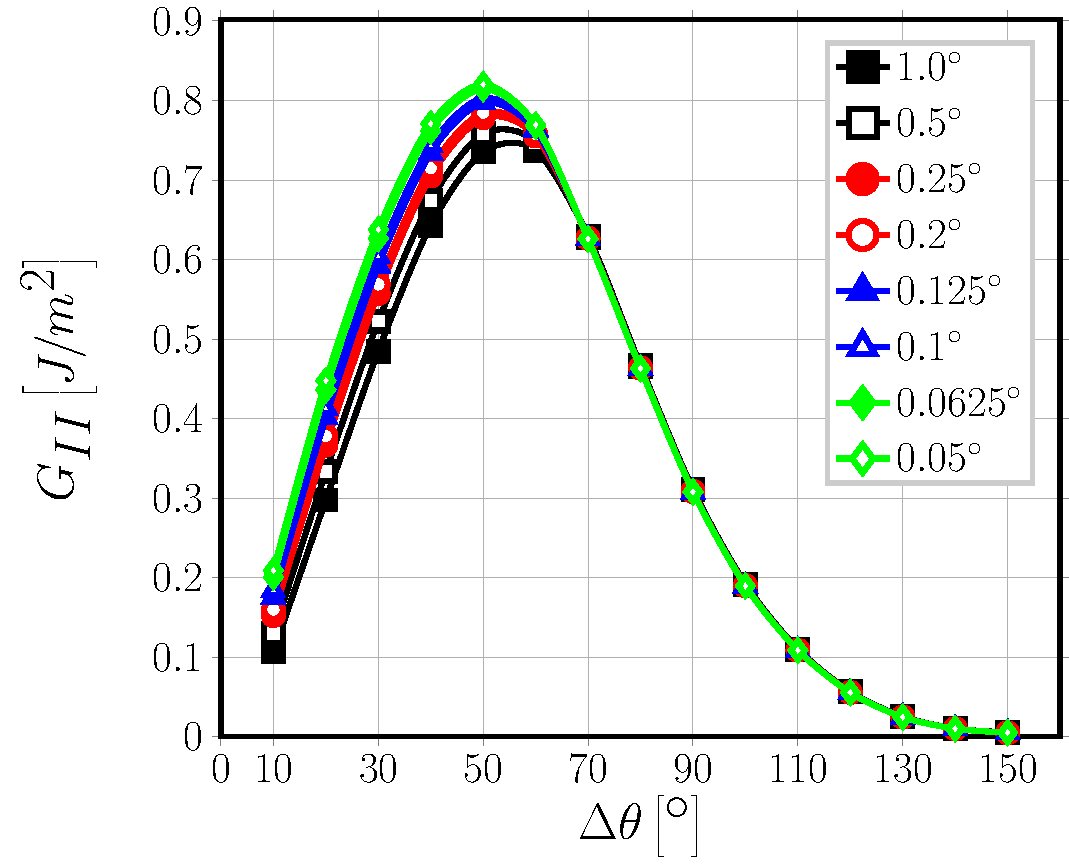
\includegraphics[width=\textwidth]{Vf40-free-1st-GII.pdf}
       \caption{$V_{f}=40\%$, $1^{st}$ order elements.}
    \end{subfigure}
    ~
    \begin{subfigure}[b]{0.48\textwidth}
        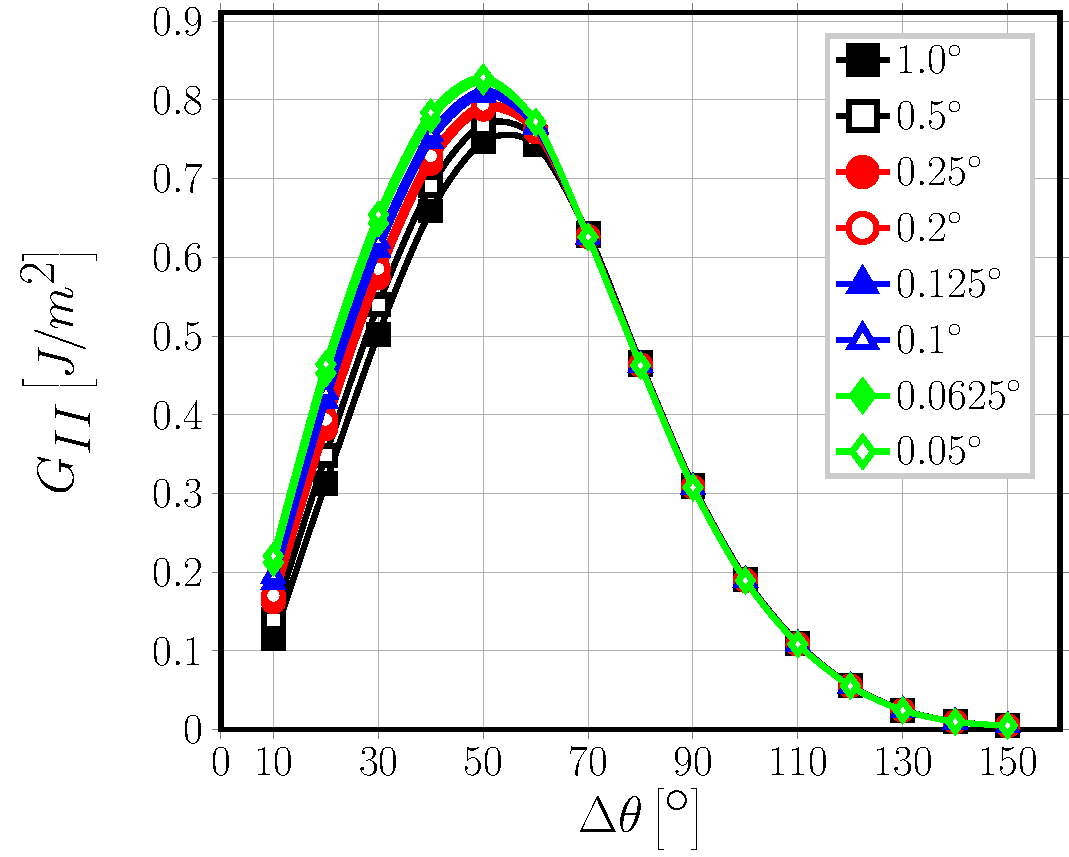
\includegraphics[width=\textwidth]{Vf40-free-2nd-GII.pdf}
       \caption{$V_{f}=40\%$, $2^{nd}$ order elements.}
    \end{subfigure}

\caption{Effect of the size $\delta$ of an element at the crack tip on Mode II ERR.}\label{fig:giinum}
\end{figure}

Observing Figure~\ref{fig:giinum}, it possible to notice the existence of two distinct regimes in the behavior of $G_{II}$ with respect to the element size $\delta$. For $\Delta\theta\leq60^{\circ}$ $G_{II}$ depends on the value of $\delta$, while $\Delta\theta\geq70^{\circ}$ it is effectively independent of the element size at the crack tip for both $1^{st}$ and $2^{nd}$ order elements and both an effectively infinite ($V_{f}=0.1\%$) and finite size ($V_{f}=40\%$) matrix. Comparing the value of $\Delta\theta$ at which the change from the $\delta$-dependency regime to the $\delta$-independency regime occurs for $G_{II}$ with Mode I ERR in Fig.~\ref{fig:ginum}, it is possible to observe that the $\delta$-dependency regime change of Mode II ERR coincides with the onset of the contact zone, i.e. the transition from \emph{open} crack regime to the \emph{closed} crack regime. The result confirms the analytical considerations of the previous section: for an \emph{open} crack both Mode I and Mode II ERR depend on the element size $\delta$ at the crack tip.

\begin{figure}[!h]
\centering
    \begin{subfigure}[b]{0.48\textwidth}
        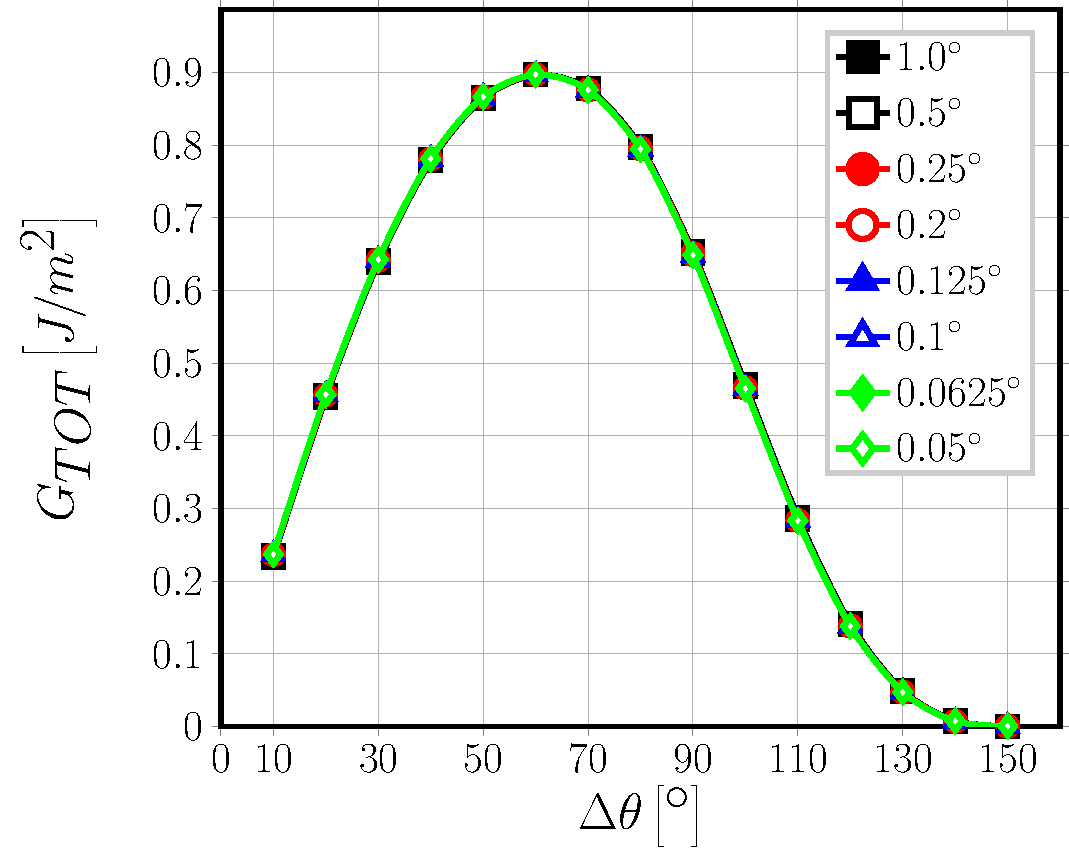
\includegraphics[width=\textwidth]{Vf0_1-free-1st-GTOT.pdf}
       \caption{$V_{f}=0.1\%$, $1^{st}$ order elements.}
    \end{subfigure}
    ~
    \begin{subfigure}[b]{0.48\textwidth}
        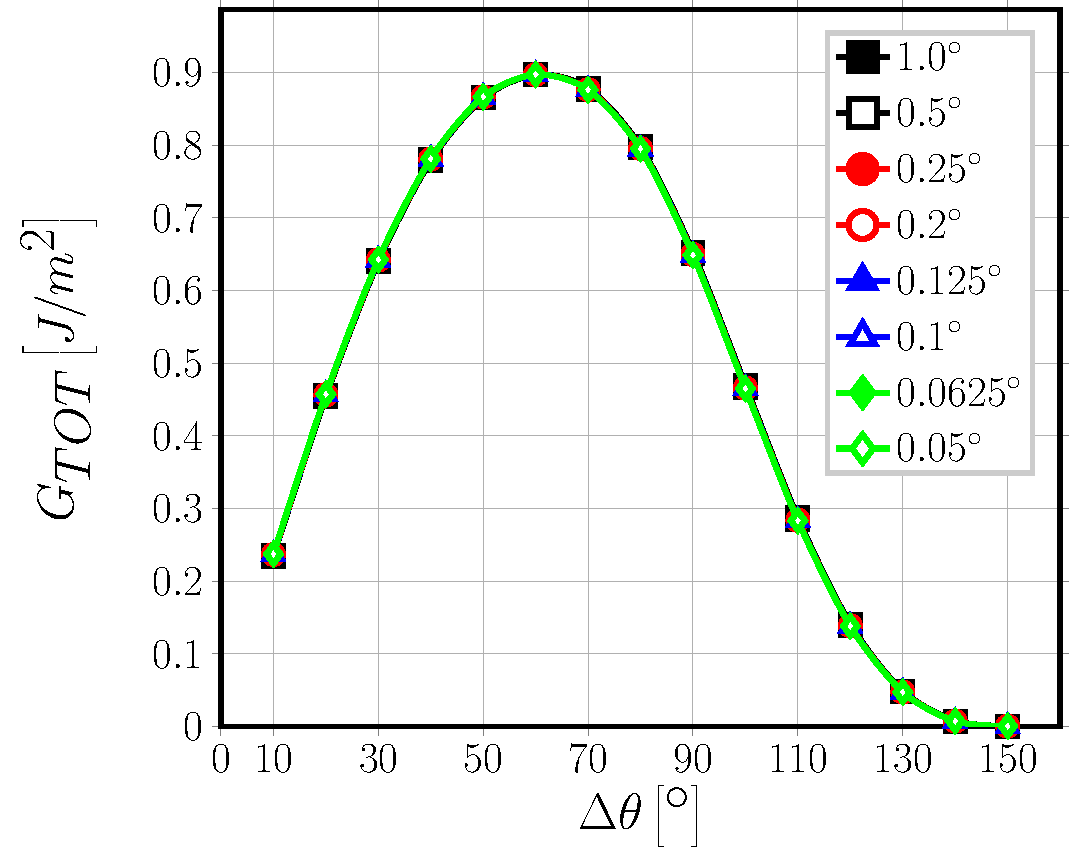
\includegraphics[width=\textwidth]{Vf0_1-free-2nd-GTOT.pdf}
       \caption{$V_{f}=0.1\%$, $2^{nd}$ order elements.}
    \end{subfigure}

    \begin{subfigure}[b]{0.48\textwidth}
        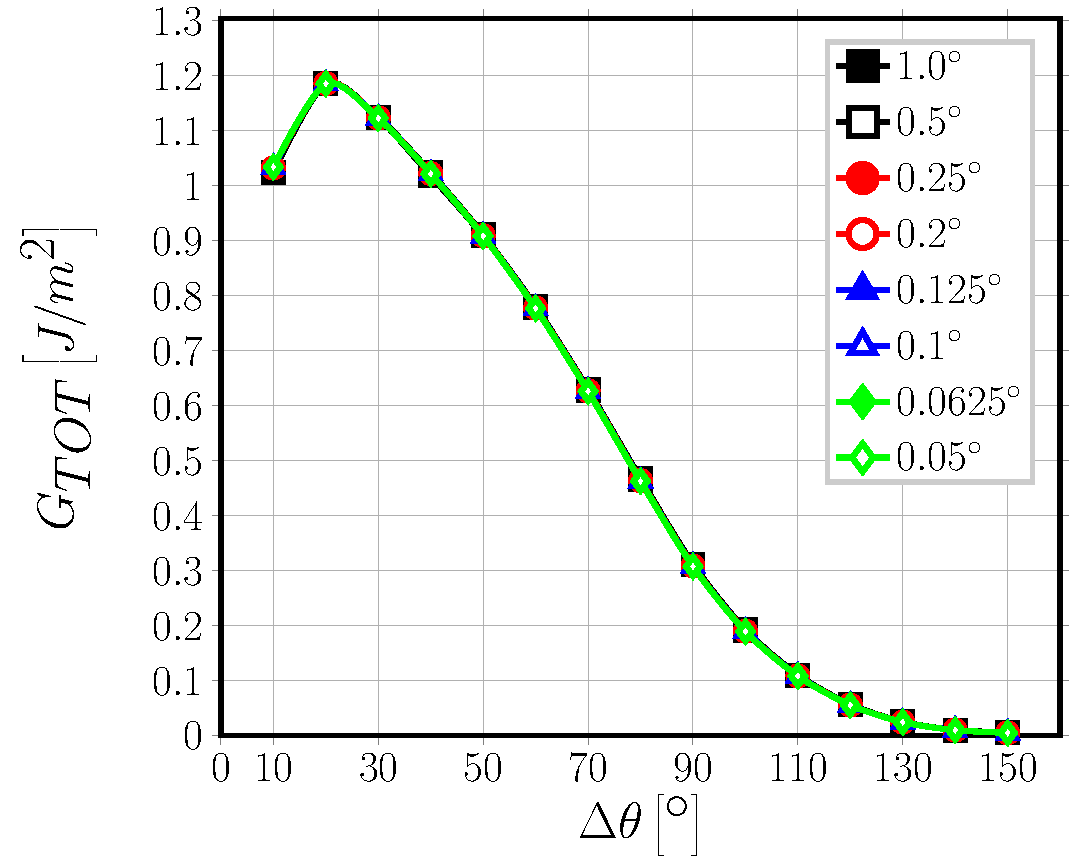
\includegraphics[width=\textwidth]{Vf40-free-1st-GTOT.pdf}
       \caption{$V_{f}=40\%$, $1^{st}$ order elements.}
    \end{subfigure}
    ~
    \begin{subfigure}[b]{0.48\textwidth}
        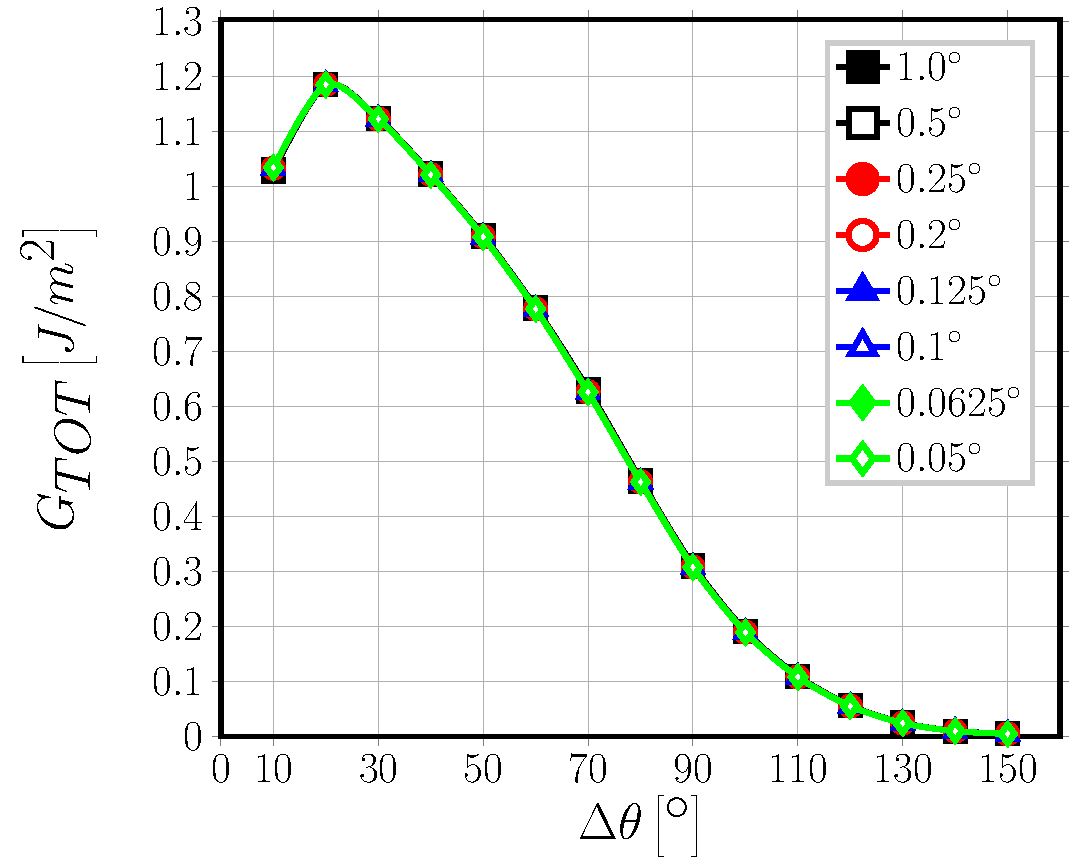
\includegraphics[width=\textwidth]{Vf40-free-2nd-GTOT.pdf}
       \caption{$V_{f}=40\%$, $2^{nd}$ order elements.}
    \end{subfigure}

\caption{Effect of the size $\delta$ of an element at the crack tip on total ERR.}\label{fig:gtotnum}
\end{figure}

Further observation of Figure~\ref{fig:giinum} reveals that, in the \emph{open} crack regime, decreasing the element size $\delta$ causes an increase of Mode II ERR. Similarly to Mode I ERR, a shift of the peak $G_{II}$ can also observed for $V_{f}=0.1\%$: the maximum value of $G_{II}$ occurs at $\Delta\theta=70^{\circ}$ for $\delta>0.25^{\circ}$ for $1^{st}$ order elements and for $\delta>0.5^{\circ}$ for $2^{nd}$ order elements, while it is shifted to $\Delta\theta=60^{\circ}$ for $\delta\leq0.25^{\circ}$ for $1^{st}$ order elements and for $\delta\leq0.5^{\circ}$ for $2^{nd}$ order elements.

\begin{table}[!h]
 \centering
 \caption{Summary of linear regression results and main statistical tests for Mode I ERR}\label{tab:GIinterp}
 \begin{tabular}{ccccccccc}
\small$\mathbf{V_{f} \left[\%\right]}$&\small\bf{Order}&\small$\mathbf{\Delta\theta \left[^{\circ}\right]}$&\small$\mathbf{A\left[\frac{J}{m^{2}}\right]}$ &\small$\mathbf{B\left[\frac{J}{m^{2}}\right]}$ &\small $\mathbf{r\left[-\right]}$ &\small $\mathbf{r^{2}\left[-\right]}$ &\small $\mathbf{p(A)\left[-\right]}$ &\small $\mathbf{p(B)\left[-\right]}$\\
\toprule
\midrule
\small0.1&\small1&	\small10.0&	\small0.0064&	\small0.2113&	\small0.9933&	\small0.9866&	\small7.48E-07&	\small3.49E-14\\
&&		\small20.0& \small0.0183&\small	0.3331&\small	0.9996&\small	0.9992&\small	1.44E-10&\small	2.40E-16\\
&&		\small30.0&	\small0.0280&\small	0.3392&\small	1.0000&\small	1.0000&\small	2.25E-16&\small	4.26E-21\\
&&		\small40.0&	\small0.0304&\small	0.2524&\small	0.9997&\small	0.9995&\small	4.38E-11&\small	7.94E-15\\
&&		\small50.0&	\small0.0235&\small	0.1278&\small	0.9985&\small	0.9970&\small	8.61E-09&\small	2.01E-11\\
&&		\small60.0&	\small0.0094&\small	0.0284&\small	0.9854&\small	0.9709&\small	7.75E-06&\small	6.14E-07\\
\midrule
\small0.1&\small2&	\small10.0&	\small0.0069&	\small0.2103&	\small0.9962&	\small0.9924&	\small1.36E-07&	\small1.03E-14\\
&&		\small20.0&	\small0.0187&\small	0.3277&\small	0.9997&\small	0.9994&\small	7.85E-11&\small	1.62E-16\\
&&		\small30.0&	\small0.0280&\small	0.3296&\small	1.0000&\small	1.0000&\small	3.28E-16&\small	7.29E-21\\
&&		\small40.0&	\small0.0298&\small	0.2408&\small	0.9997&\small	0.9995&\small	4.82E-11&\small	1.04E-14\\
&&		\small50.0&	\small0.0225&\small	0.1177&\small	0.9984&\small	0.9967&\small	1.10E-08&\small	3.27E-11\\
&&		\small60.0&	\small0.0081&\small	0.0228&\small	0.9811&\small	0.9626&\small	1.66E-05&\small	2.17E-06\\
\midrule
\small40&\small1&	\small10.0&	\small0.0311&	\small0.9196&	\small0.9963&	\small0.9927&	\small1.03E-07&	\small9.33E-15\\
&&		\small20.0&	\small0.0501&\small	0.8882&\small	1.0000&\small	0.9999&\small	1.21E-13&\small	2.33E-19\\
&&		\small30.0&	\small0.0510&\small	0.6374&\small	0.9998&\small	0.9996&\small	1.66E-11&\small	2.58E-16\\
&&		\small40.0&	\small0.0419&\small	0.3760&\small	0.9988&\small	0.9976&\small	4.56E-09&\small	5.25E-13\\
&&		\small50.0&	\small0.0279&\small	0.1713&\small	0.9980&\small	0.9961&\small	2.22E-08&\small	2.52E-11\\
&&		\small60.0&	\small0.0108&\small	0.0391&\small	0.9901&\small	0.9804&\small	3.44E-06&\small	9.46E-08\\
\midrule
\small40&\small2&	\small10.0&	\small0.0336&	\small0.9148&	\small0.9988&	\small0.9977&	\small3.45E-09&	\small5.09E-16\\
&&		\small20.0&	\small0.0504&\small	0.8719&\small	1.0000&\small	1.0000&\small	3.70E-14&\small	8.26E-20\\
&&		\small30.0&	\small0.0506&\small	0.6191&\small	0.9999&\small	0.9997&\small	7.63E-12&\small	1.35E-16\\
&&		\small40.0&	\small0.0414&\small	0.3608&\small	0.9994&\small	0.9989&\small	4.95E-10&\small	6.80E-14\\
&&		\small50.0&	\small0.0269&\small	0.1593&\small	0.9982&\small	0.9964&\small	1.66E-08&\small	2.31E-11\\
&&		\small60.0&	\small0.0097&\small	0.0329&\small	0.9890&\small	0.9781&\small	4.96E-06&\small	1.99E-07\\
\end{tabular}
\end{table}

Analysis of the total ERR in Figure~\ref{fig:gtotnum} leads to an observation that was not predicted by the considerations of the previous section: $G_{TOT}$ is effectively independent of the element size $\delta$ in both the \emph{open} and the \emph{closed} crack regimes, at least for reasonably small elements ($\delta\leq1.0^{\circ}$). Given that $G_{II}=G_{TOT}$ for the \emph{closed} crack, it explains the independency of $G_{II}$ from $\delta$ after the onset of the contact zone.

\begin{table}[!h]
 \centering
 \caption{Summary of linear regression results and main statistical tests for Mode II ERR}\label{tab:GIIinterp}
 \begin{tabular}{ccccccccc}
\small$\mathbf{V_{f} \left[\%\right]}$&\small\bf{Order}&\small$\mathbf{\Delta\theta \left[^{\circ}\right]}$&\small$\mathbf{A\left[\frac{J}{m^{2}}\right]}$ &\small$\mathbf{B\left[\frac{J}{m^{2}}\right]}$ &\small $\mathbf{r\left[-\right]}$ &\small $\mathbf{r^{2}\left[-\right]}$ &\small $\mathbf{p(A)\left[-\right]}$ &\small $\mathbf{p(B)\left[-\right]}$\\
\toprule
\midrule
\small0.1&\small	1.0&\small	10.0&\small	-0.0076&\small	0.0228&\small	-0.9996&\small	0.9991&\small	2.09E-10&\small	1.64E-11\\
&\small&\small		20.0&\small	-0.0194&\small	0.1211&\small	-1.0000&\small	1.0000&\small	1.99E-15&\small	2.02E-18\\
&\small&\small		30.0&\small	-0.0290&\small	0.3007&\small	-0.9999&\small	0.9998&\small	4.12E-12&\small	1.97E-16\\
&\small&\small		40.0&\small	-0.0311&\small	0.5270&\small	-0.9995&\small	0.9989&\small	4.13E-10&\small	1.05E-15\\
&\small&\small		50.0&\small	-0.0240&\small	0.7375&\small	-0.9979&\small	0.9958&\small	2.32E-08&\small	1.66E-15\\
&\small&\small		60.0&\small	-0.0095&\small	0.8685&\small	-0.9835&\small	0.9672&\small	1.12E-05&\small	1.22E-15\\
\midrule
\small0.1&\small	2.0&\small	10.0&\small	-0.0078&\small	0.0249&\small	-0.9996&\small	0.9992&\small	1.91E-10&\small	1.06E-11\\
&\small&\small		20.0&\small	-0.0196&\small	0.1272&\small	-1.0000&\small	1.0000&\small	3.48E-15&\small	2.78E-18\\
&\small&\small		30.0&\small	-0.0288&\small	0.3108&\small	-0.9999&\small	0.9998&\small	1.45E-12&\small	5.47E-17\\
&\small&\small		40.0&\small	-0.0305&\small	0.5387&\small	-0.9995&\small	0.9990&\small	3.32E-10&\small	6.55E-16\\
&\small&\small		50.0&\small	-0.0229&\small	0.7478&\small	-0.9979&\small	0.9959&\small	2.17E-08&\small	1.09E-15\\
&\small&\small		60.0&\small	-0.0082&\small	0.8744&\small	-0.9806&\small	0.9615&\small	1.81E-05&\small	8.26E-16\\
\midrule
\small40.0&\small	1.0&\small	10.0&\small	-0.0344&\small	0.1055&\small	-0.9997&\small	0.9995&\small	3.82E-11&\small	2.73E-12\\
&\small&\small		20.0&\small	-0.0500&\small	0.2977&\small	-1.0000&\small	0.9999&\small	4.22E-14&\small	5.66E-17\\
&\small&\small		30.0&\small	-0.0505&\small	0.4866&\small	-0.9999&\small	0.9997&\small	6.44E-12&\small	4.82E-16\\
&\small&\small		40.0&\small	-0.0420&\small	0.6454&\small	-0.9996&\small	0.9991&\small	2.12E-10&\small	9.66E-16\\
&\small&\small		50.0&\small	-0.0275&\small	0.7386&\small	-0.9985&\small	0.9971&\small	9.01E-09&\small	1.44E-15\\
&\small&\small		60.0&\small	-0.0099&\small	0.7402&\small	-0.9926&\small	0.9853&\small	1.41E-06&\small	5.13E-16\\
\midrule
\small40.0&\small	2.0&\small	10.0&\small	-0.0353&\small	0.1145&\small	-0.9998&\small	0.9995&\small	2.92E-11&\small	1.50E-12\\
&\small&\small		20.0&\small	-0.0504&\small	0.3130&\small	-1.0000&\small	0.9999&\small	4.00E-14&\small	4.17E-17\\
&\small&\small		30.0&\small	-0.0502&\small	0.5039&\small	-0.9999&\small	0.9998&\small	2.87E-12&\small	1.69E-16\\
&\small&\small		40.0&\small	-0.0410&\small	0.6615&\small	-0.9996&\small	0.9992&\small	2.02E-10&\small	6.89E-16\\
&\small&\small		50.0&\small	-0.0263&\small	0.7502&\small	-0.9987&\small	0.9973&\small	6.87E-09&\small	7.76E-16\\
&\small&\small		60.0&\small	-0.0090&\small	0.7458&\small	-0.9921&\small	0.9842&\small	1.79E-06&\small	3.37E-16\\
\end{tabular}
\end{table}

Analysis of Fig.~\ref{fig:ginum}, Fig.~\ref{fig:giinum} and Fig.~\ref{fig:gtotnum} has shown the dependency of Mode I and Mode II ERR on the element size $\delta$. Following the derivations of the previous section, we model the dependency of $G_{I}$ and $G_{II}$ with respect to $\delta$ as

\begin{equation}
G_{\left(\cdot\right)}=A\left(\Delta\theta\right)\ln\delta+B\left(\Delta\theta\right),
\end{equation}

where $A\left(\Delta\theta\right)$ and $B\left(\Delta\theta\right)$ are parameters dependent on $\Delta\theta$ estimated through linear regression (with $x=\ln\delta$) of the numerical results.

\begin{figure}[!h]
\centering
    \begin{subfigure}[b]{0.48\textwidth}
        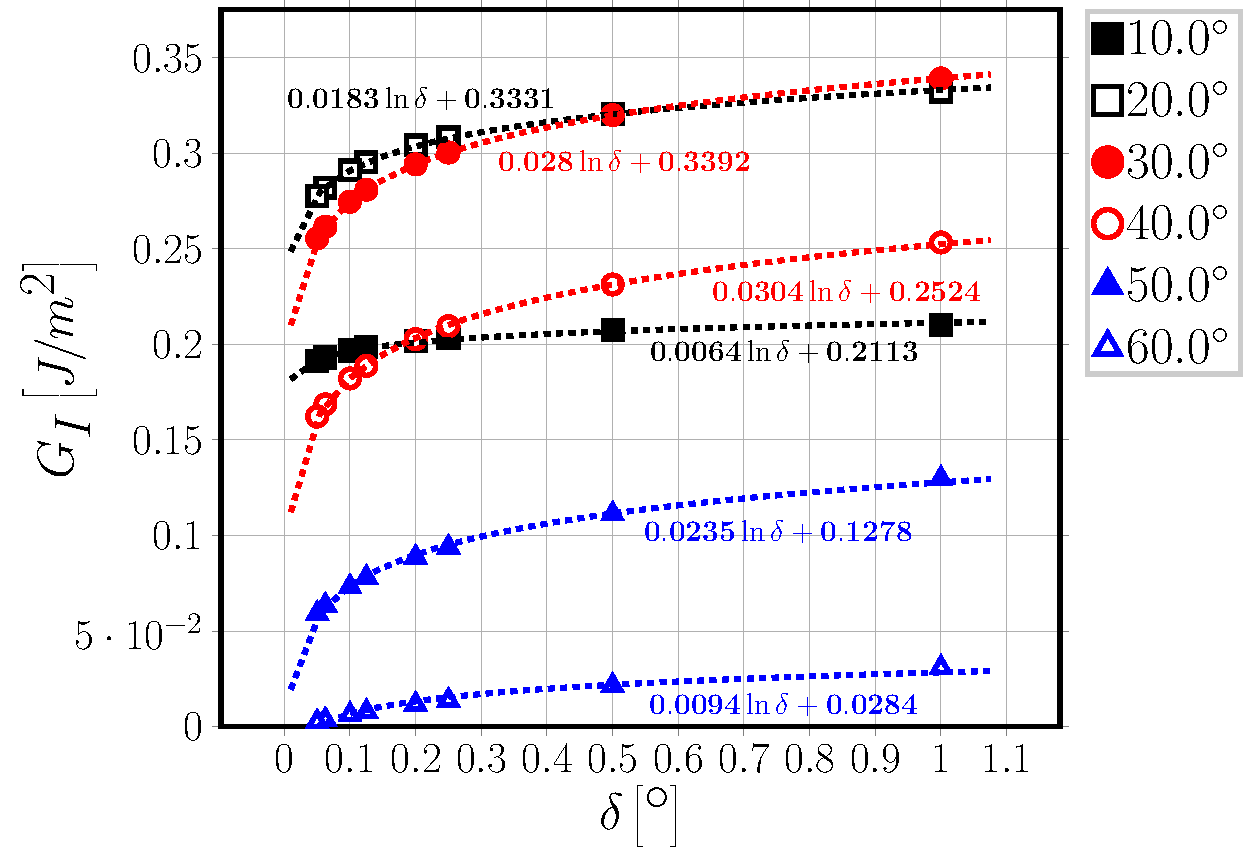
\includegraphics[width=\textwidth]{Vf0_1-free-1st-vsDelta-GI.pdf}
       \caption{$1^{st}$ order elements.}
    \end{subfigure}
    ~
    \begin{subfigure}[b]{0.48\textwidth}
        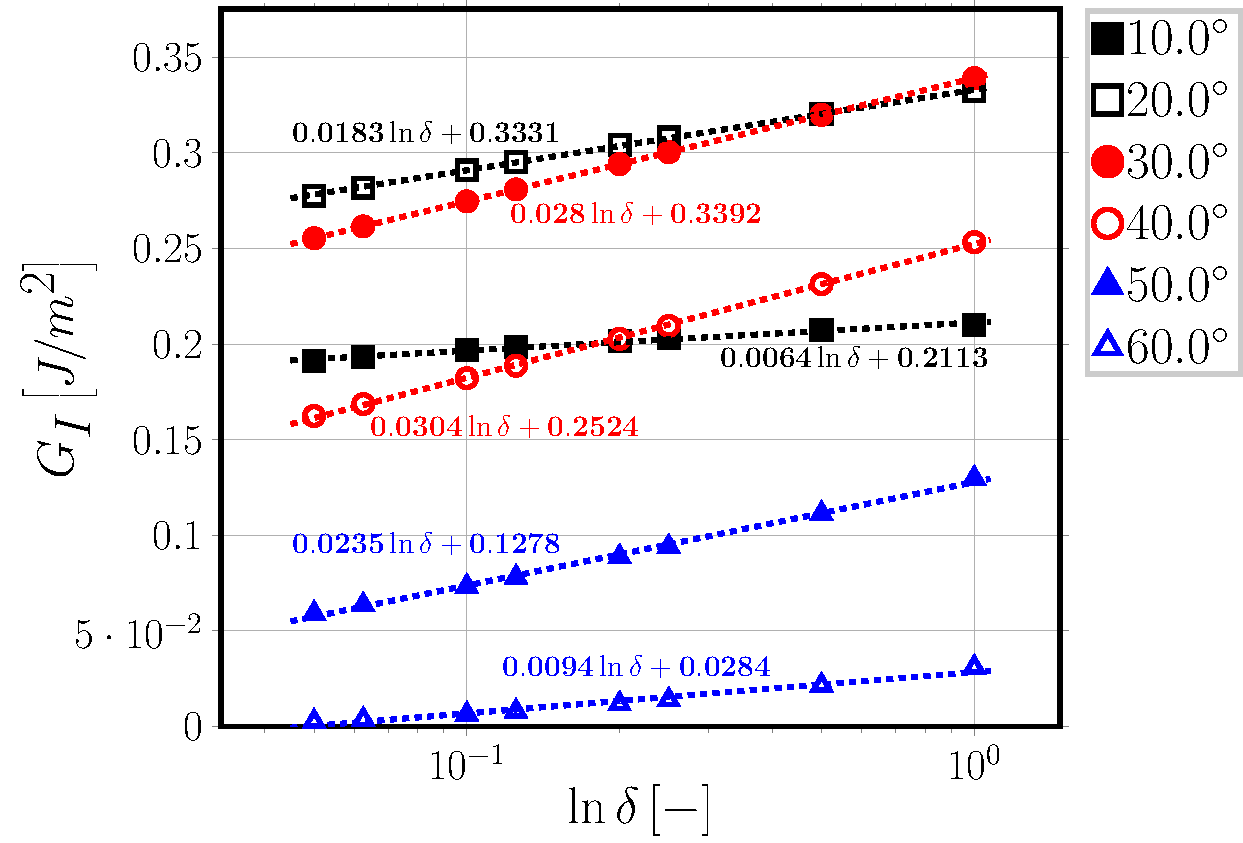
\includegraphics[width=\textwidth]{Vf0_1-free-1st-semilogvsDelta-GI.pdf}
       \caption{$1^{st}$ order elements.}
    \end{subfigure}

    \begin{subfigure}[b]{0.48\textwidth}
        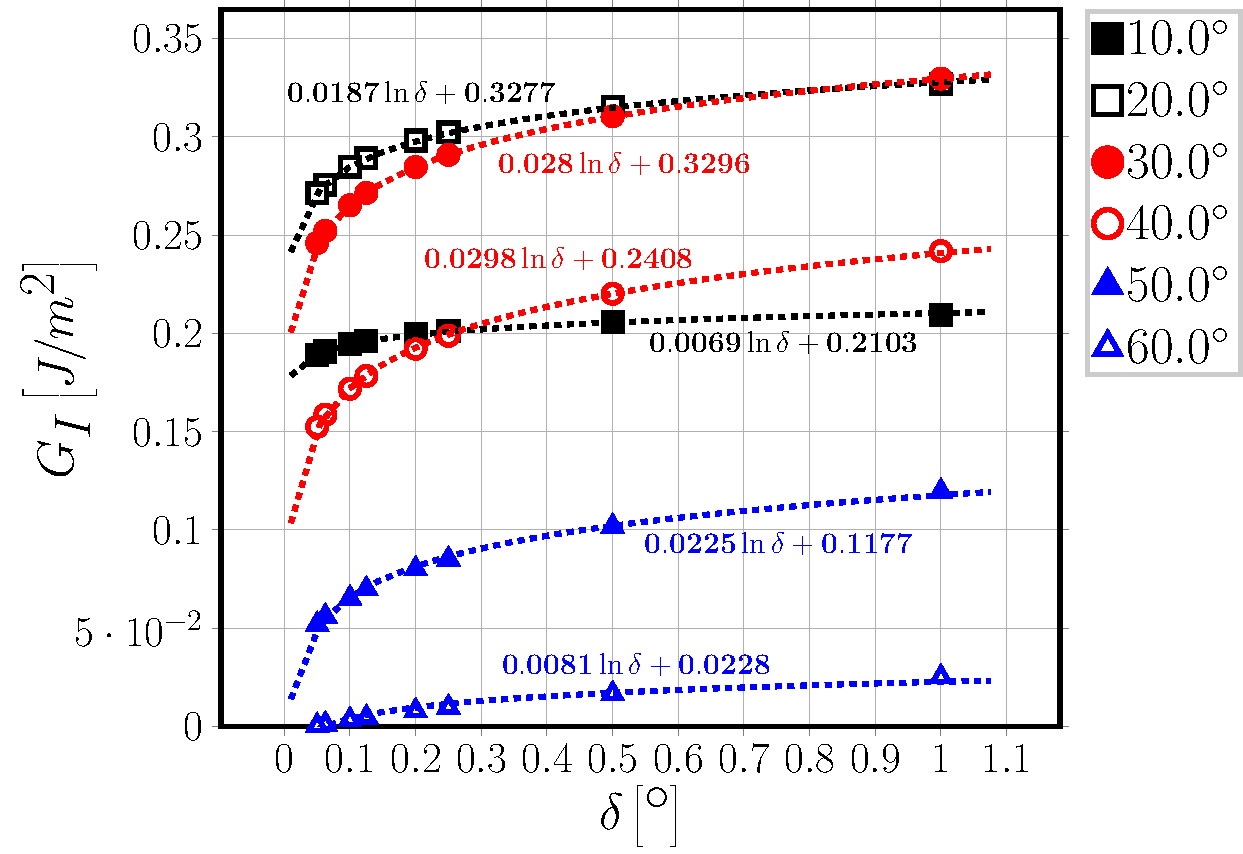
\includegraphics[width=\textwidth]{Vf0_1-free-2nd-vsDelta-GI.pdf}
       \caption{$2^{nd}$ order elements.}
    \end{subfigure}
    ~
    \begin{subfigure}[b]{0.48\textwidth}
        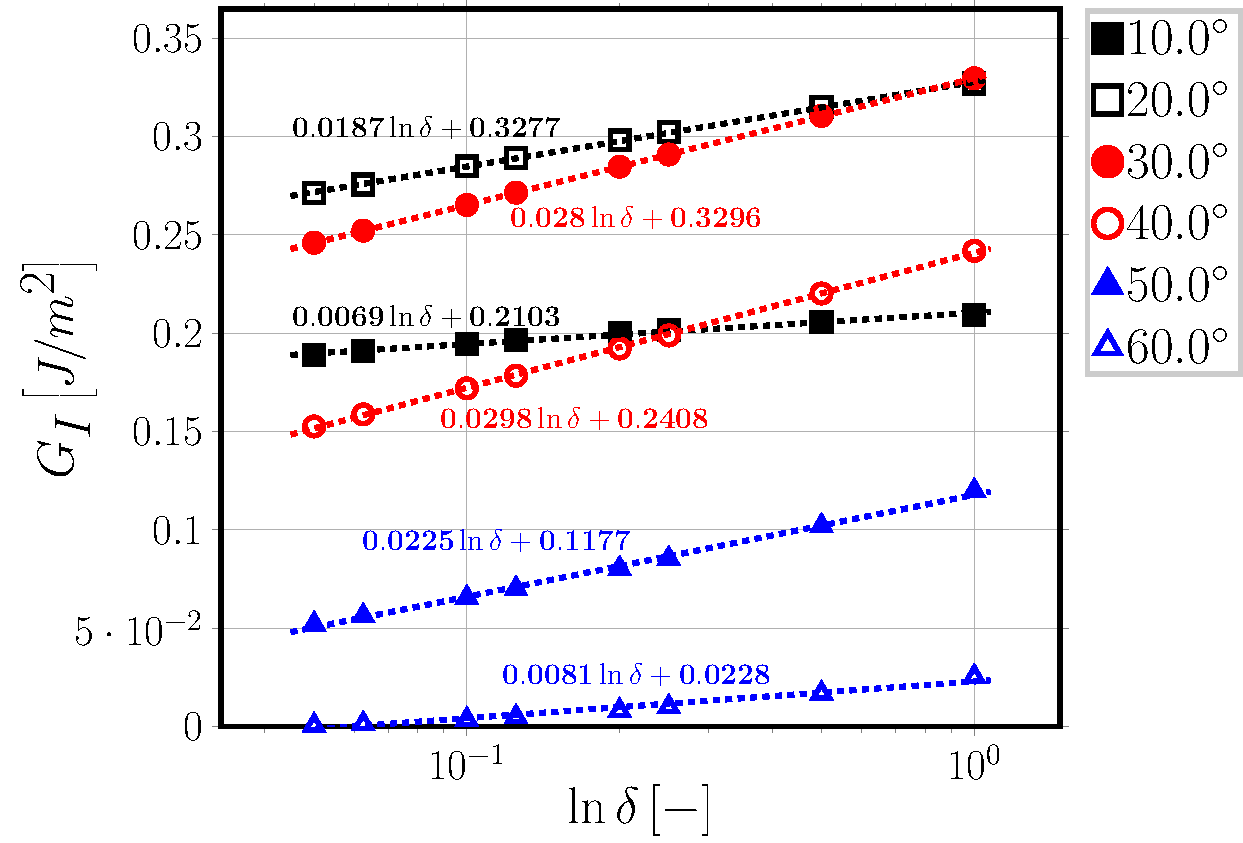
\includegraphics[width=\textwidth]{Vf0_1-free-2nd-semilogvsDelta-GI.pdf}
       \caption{$2^{nd}$ order elements.}
    \end{subfigure}

\caption{Logarithmic dependence on $\delta$ of Mode I ERR: interpolation of numerical results for $V_{f}=0.1\%$.}\label{fig:giinterp01}
\end{figure}

\begin{figure}[!h]
\centering
    \begin{subfigure}[b]{0.48\textwidth}
        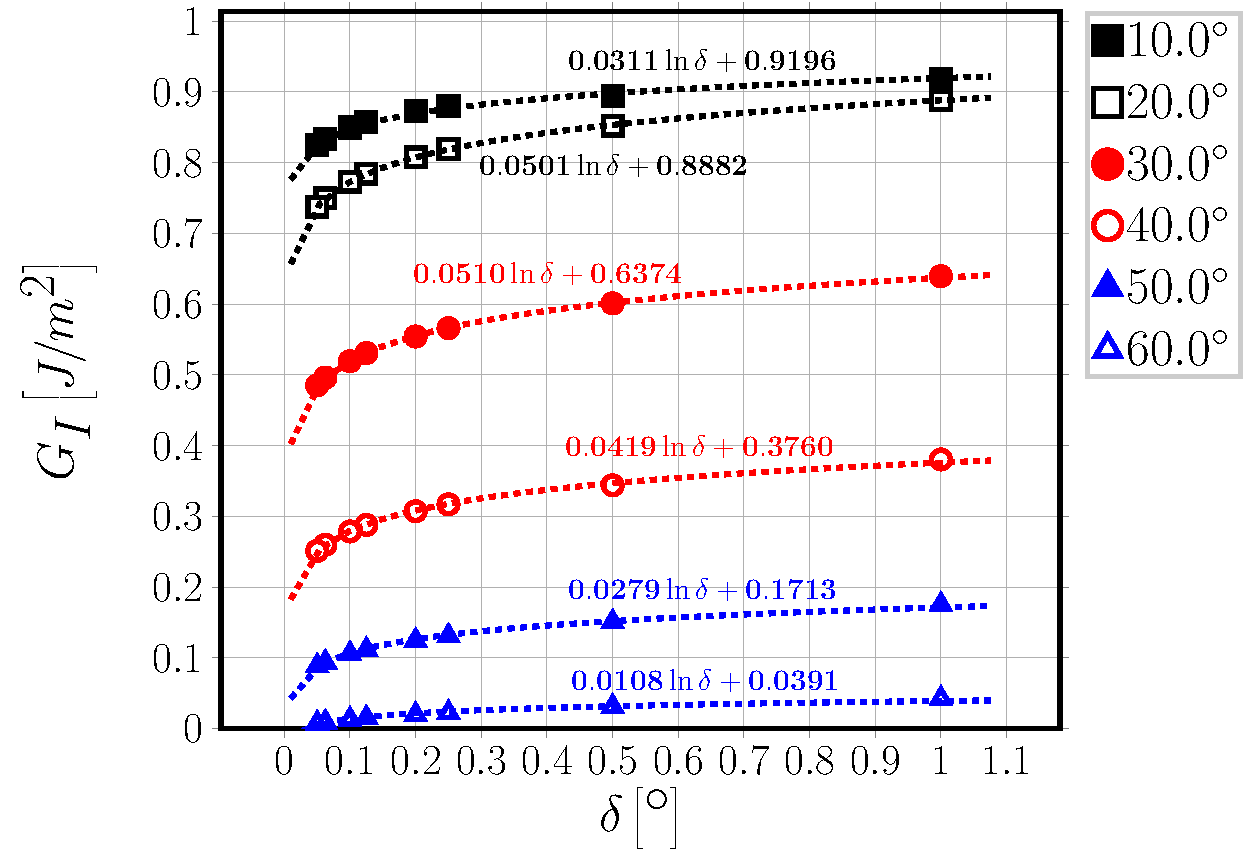
\includegraphics[width=\textwidth]{Vf40-free-1st-vsDelta-GI.pdf}
       \caption{$1^{st}$ order elements.}
    \end{subfigure}
    ~
    \begin{subfigure}[b]{0.48\textwidth}
        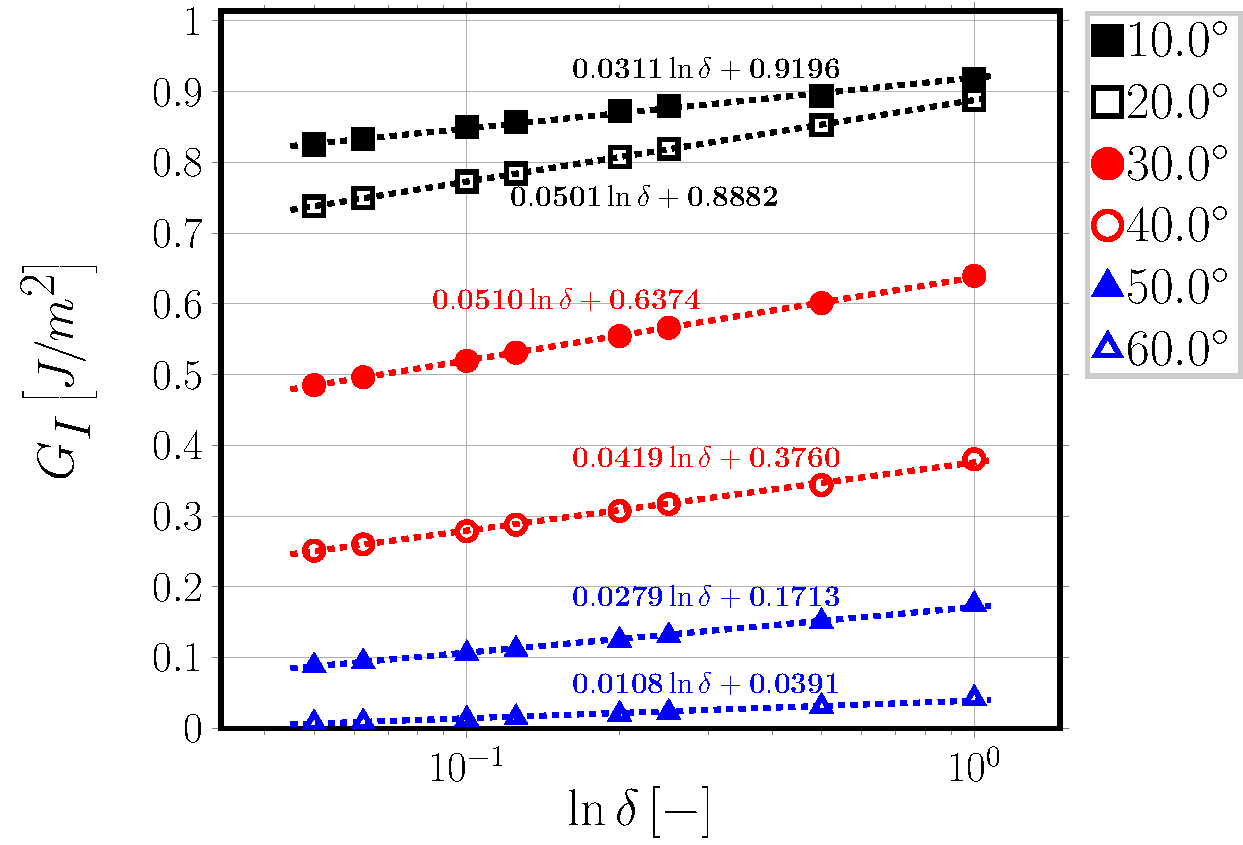
\includegraphics[width=\textwidth]{Vf40-free-1st-semilogvsDelta-GI.pdf}
       \caption{$1^{st}$ order elements.}
    \end{subfigure}

    \begin{subfigure}[b]{0.48\textwidth}
        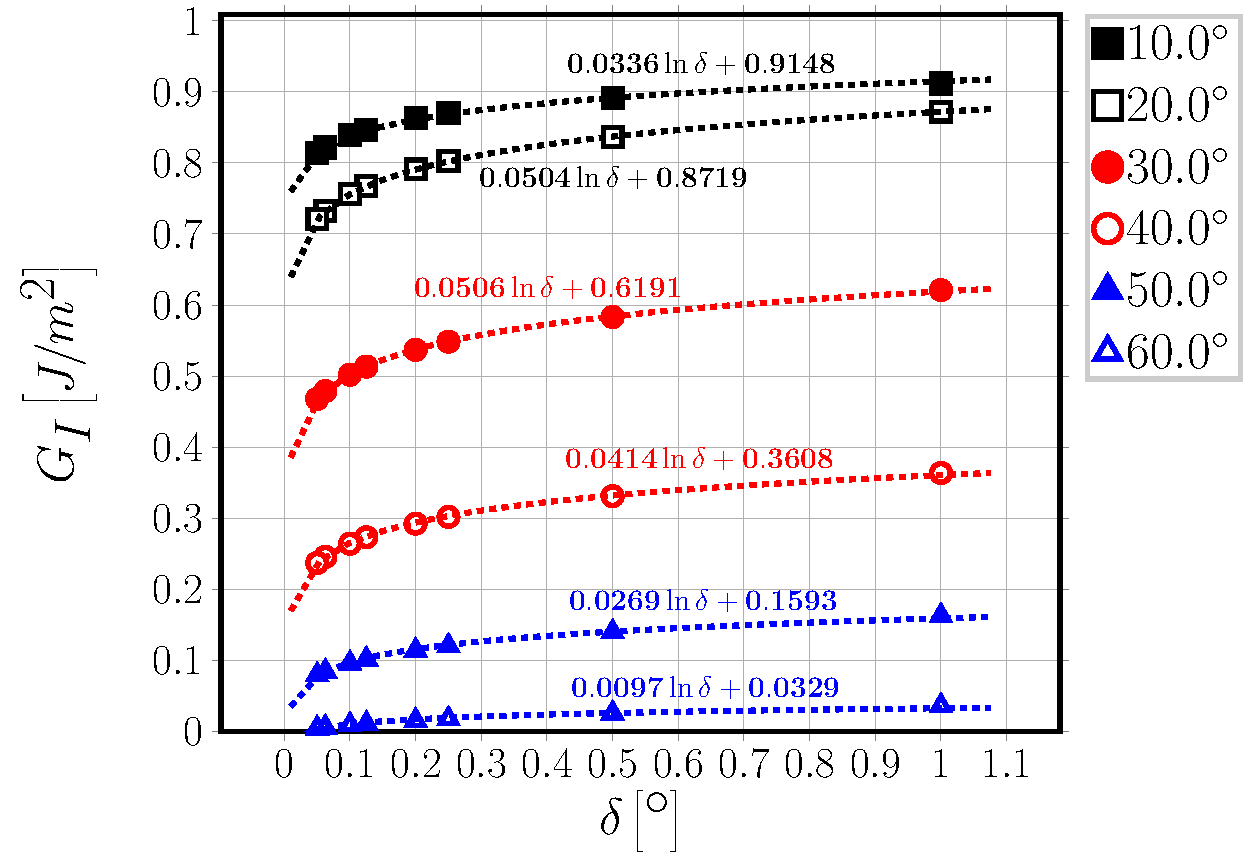
\includegraphics[width=\textwidth]{Vf40-free-2nd-vsDelta-GI.pdf}
       \caption{$2^{nd}$ order elements.}
    \end{subfigure}
    ~
    \begin{subfigure}[b]{0.48\textwidth}
        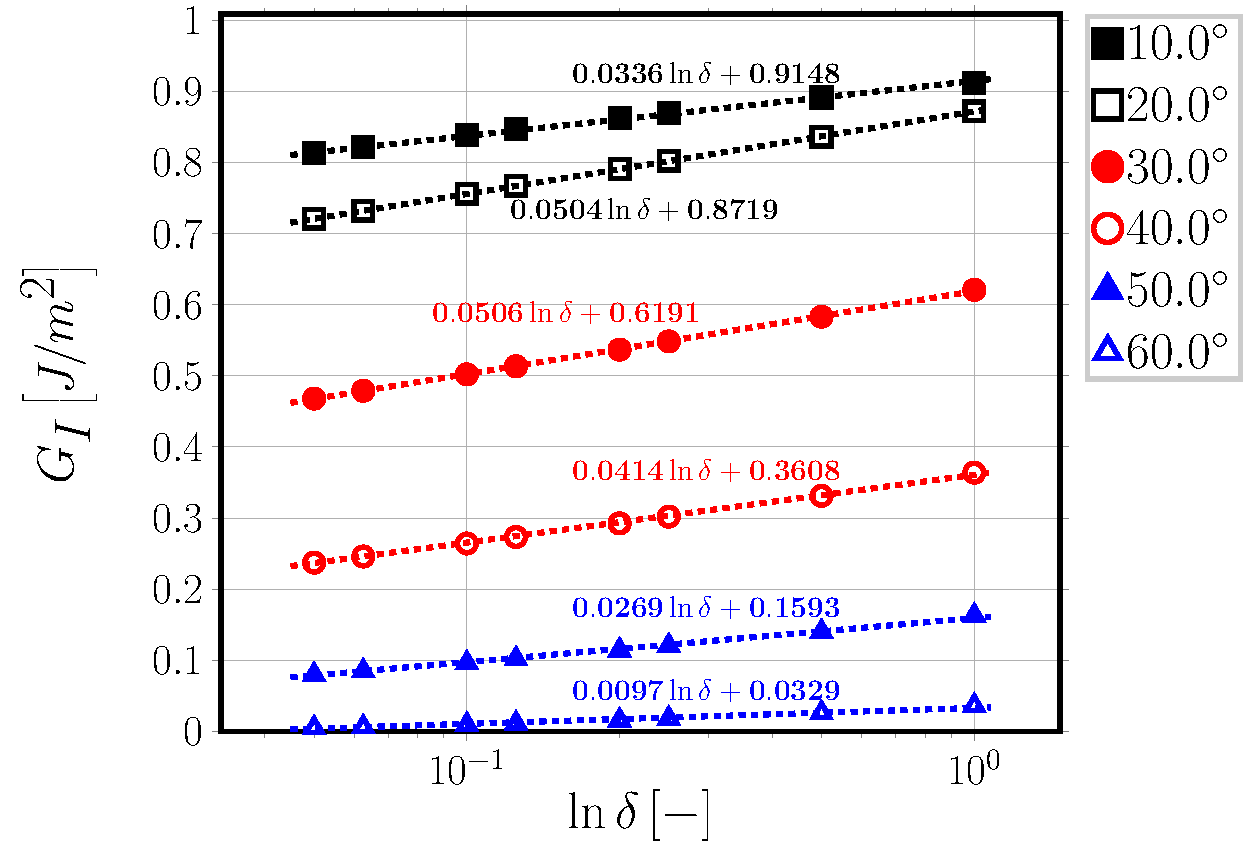
\includegraphics[width=\textwidth]{Vf40-free-2nd-semilogvsDelta-GI.pdf}
       \caption{$2^{nd}$ order elements.}
    \end{subfigure}

\caption{Logarithmic dependence on $\delta$ of Mode I ERR: interpolation of numerical results for $V_{f}=40\%$.}\label{fig:giinterp40}
\end{figure}

\begin{figure}[!h]
\centering
    \begin{subfigure}[b]{0.48\textwidth}
        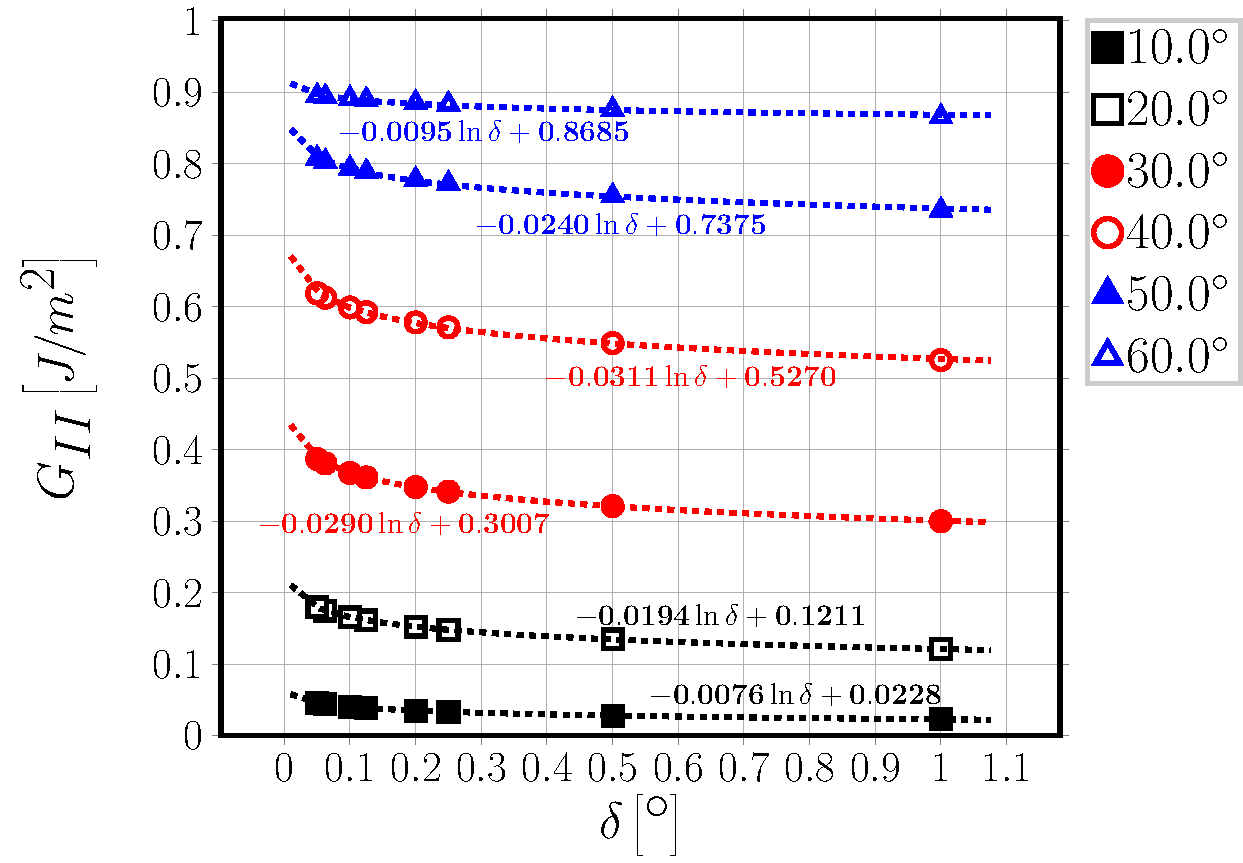
\includegraphics[width=\textwidth]{Vf0_1-free-1st-vsDelta-GII.pdf}
       \caption{$1^{st}$ order elements.}
    \end{subfigure}
    ~
    \begin{subfigure}[b]{0.48\textwidth}
        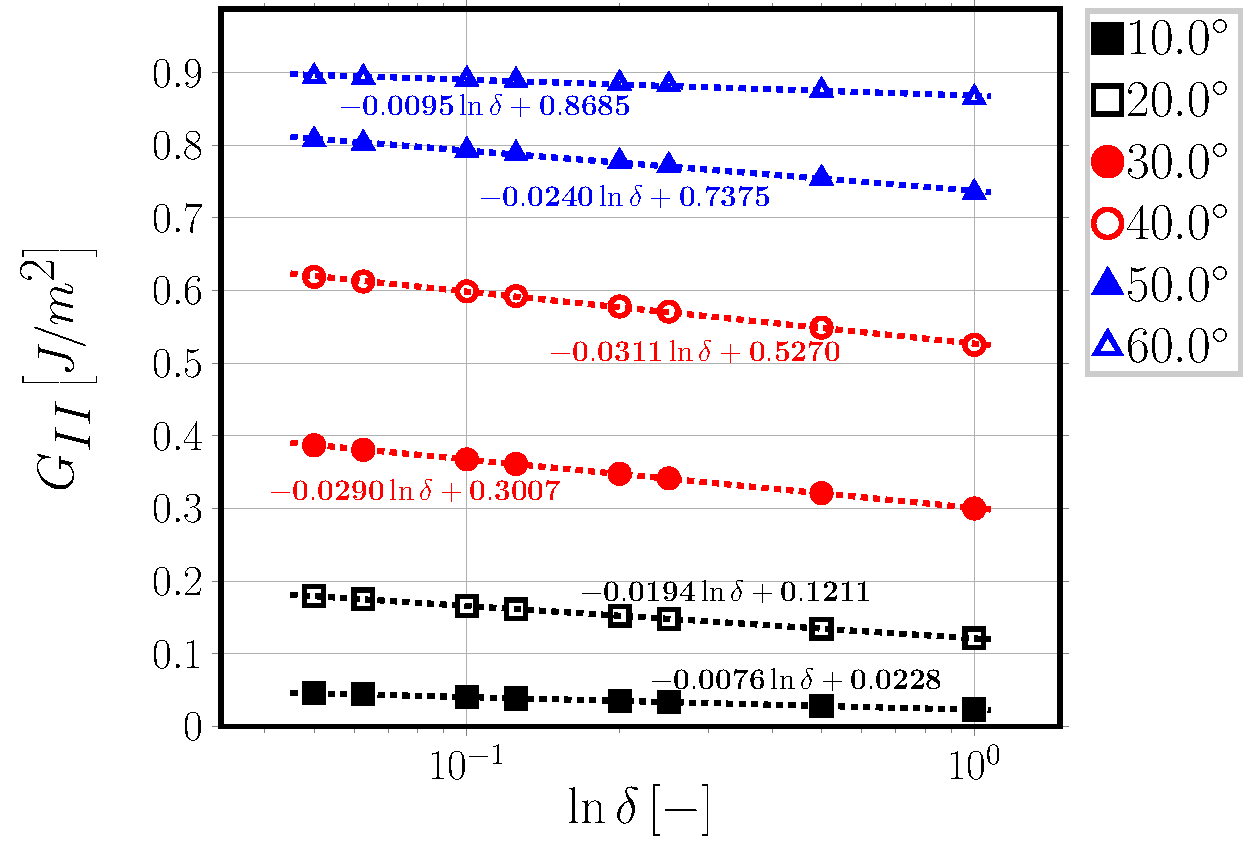
\includegraphics[width=\textwidth]{Vf0_1-free-1st-semilogvsDelta-GII.pdf}
       \caption{$1^{st}$ order elements.}
    \end{subfigure}

    \begin{subfigure}[b]{0.48\textwidth}
        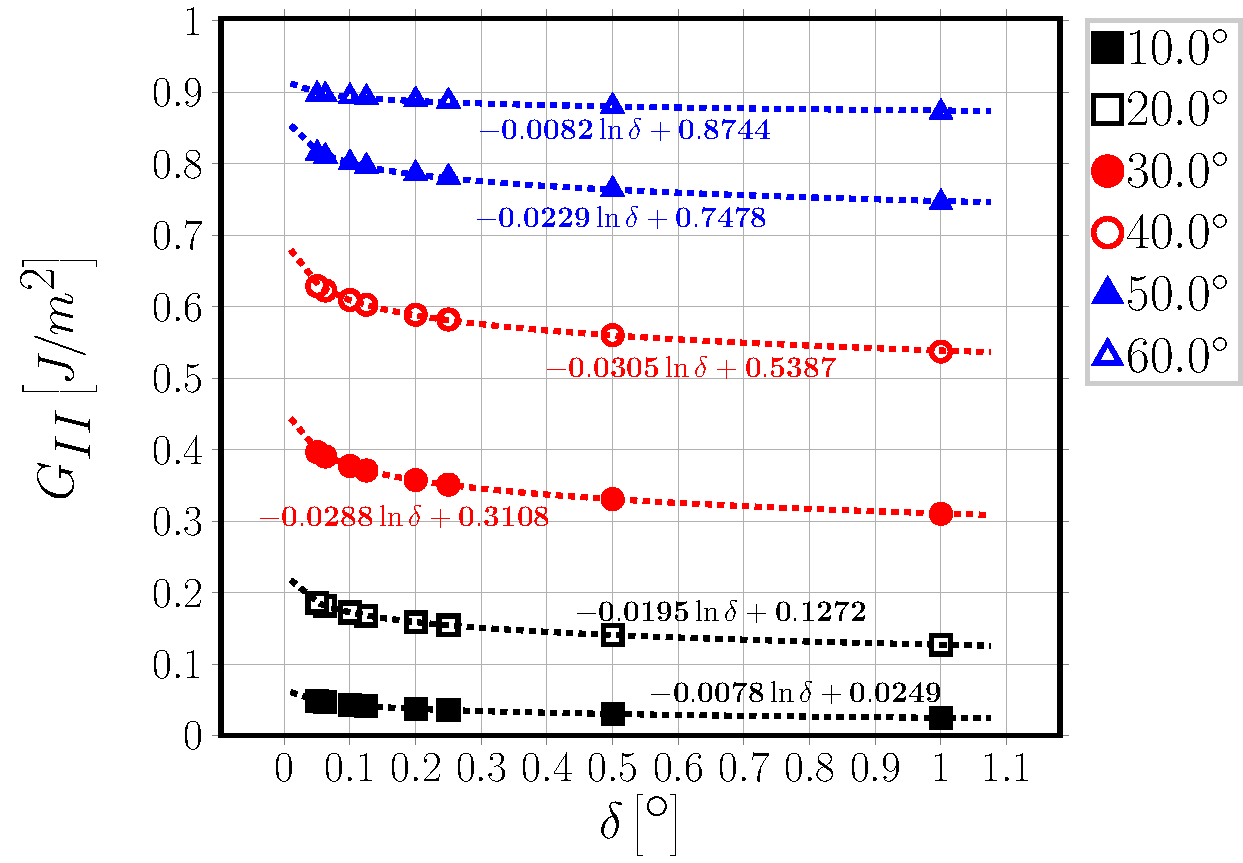
\includegraphics[width=\textwidth]{Vf0_1-free-2nd-vsDelta-GII.pdf}
       \caption{$2^{nd}$ order elements.}
    \end{subfigure}
    ~
    \begin{subfigure}[b]{0.48\textwidth}
        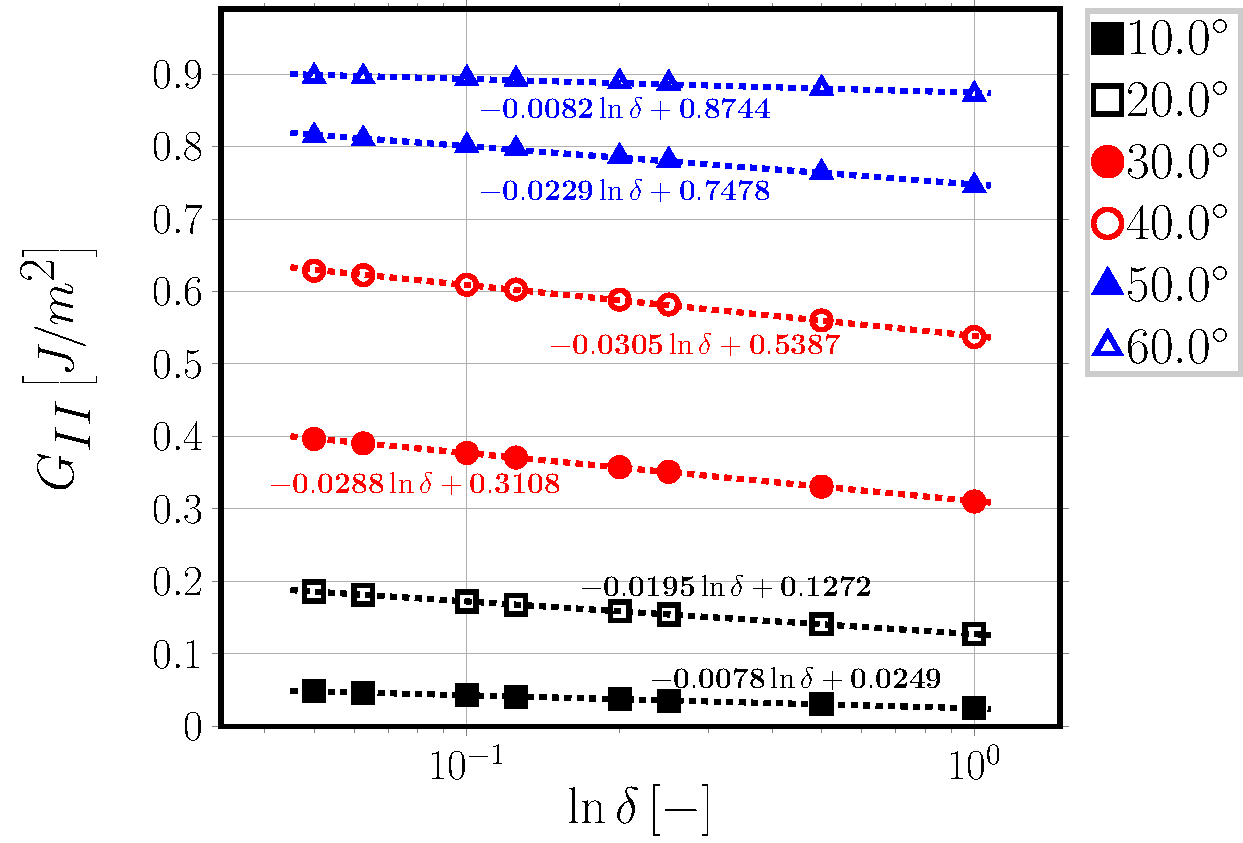
\includegraphics[width=\textwidth]{Vf0_1-free-2nd-semilogvsDelta-GII.pdf}
       \caption{$2^{nd}$ order elements.}
    \end{subfigure}

\caption{Logarithmic dependence on $\delta$ of Mode II ERR: interpolation of numerical results for $V_{f}=0.1\%$.}\label{fig:giiinterp01}
\end{figure}

\begin{figure}[!h]
\centering
    \begin{subfigure}[b]{0.48\textwidth}
        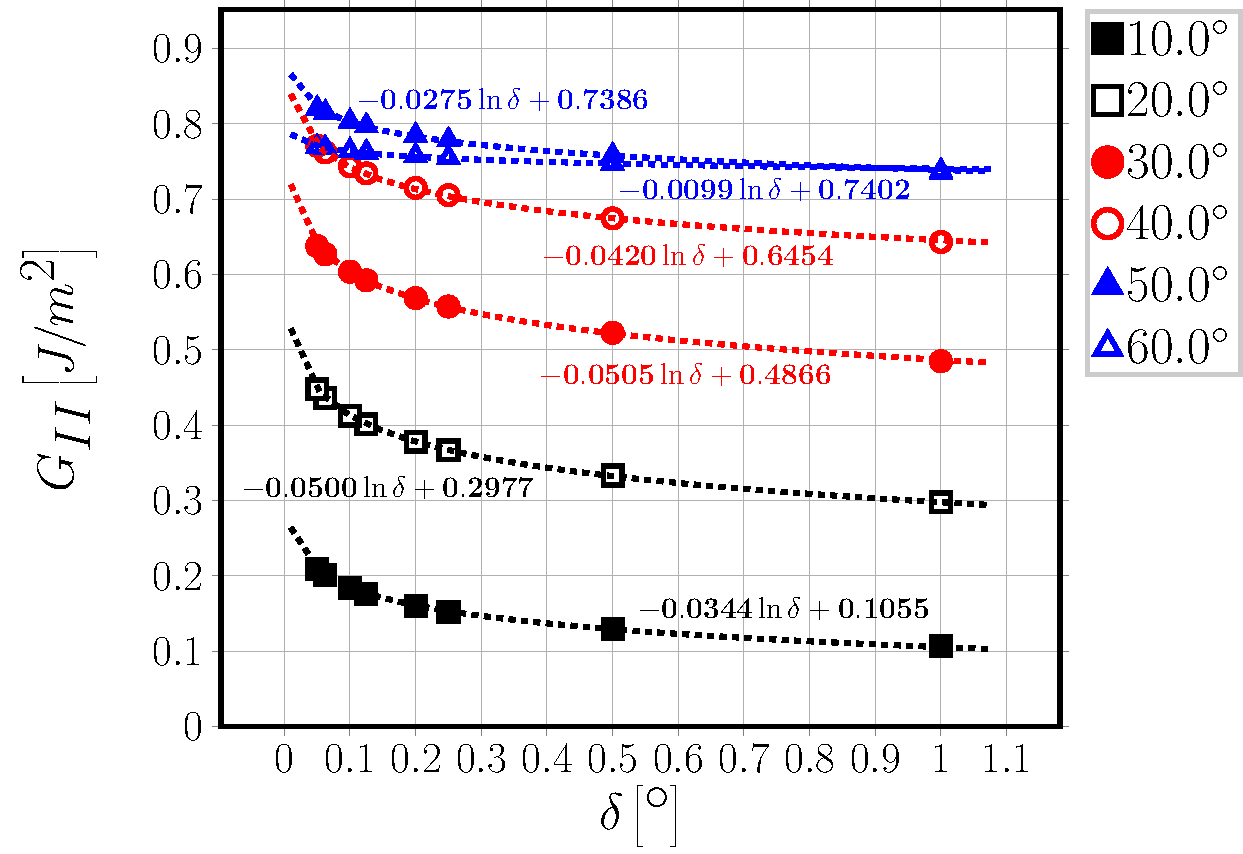
\includegraphics[width=\textwidth]{Vf40-free-1st-vsDelta-GII.pdf}
       \caption{$1^{st}$ order elements.}
    \end{subfigure}
    ~
    \begin{subfigure}[b]{0.48\textwidth}
        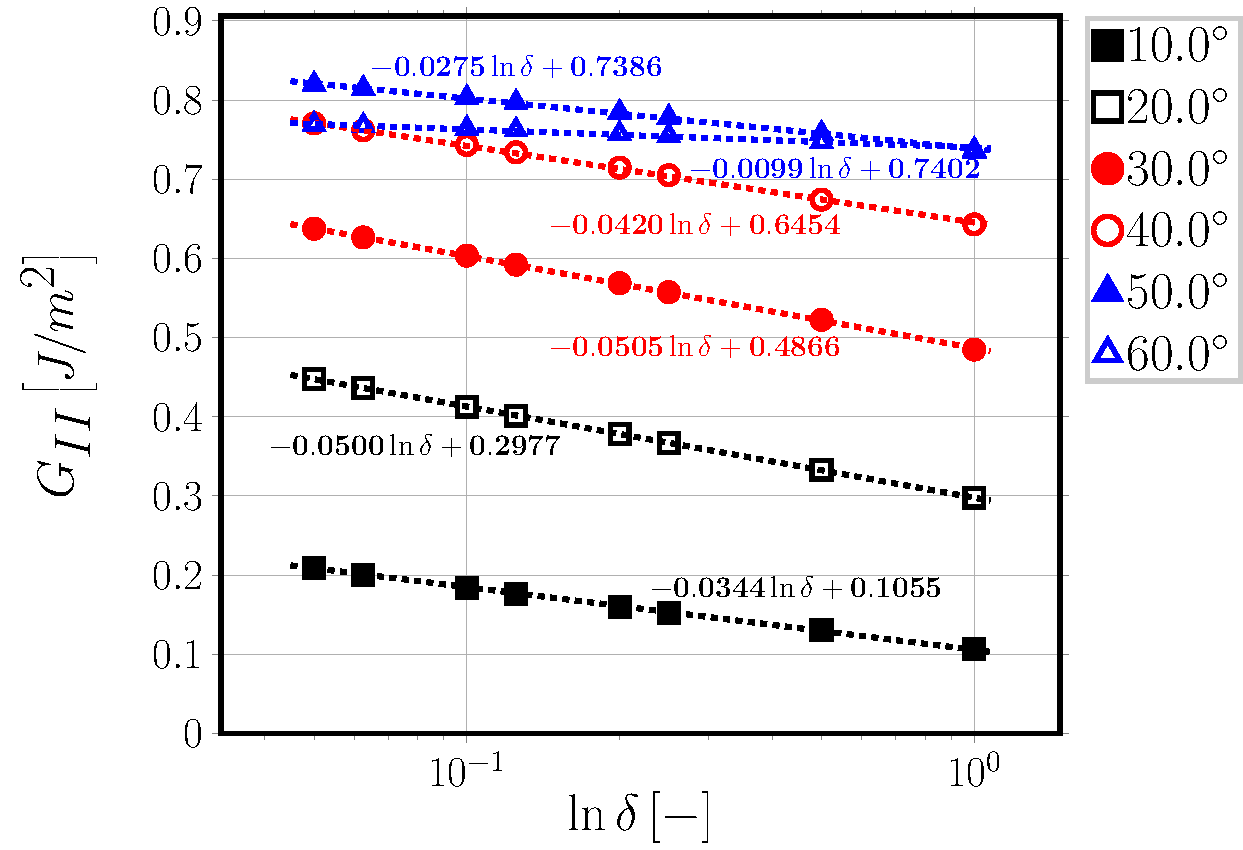
\includegraphics[width=\textwidth]{Vf40-free-1st-semilogvsDelta-GII.pdf}
       \caption{$1^{st}$ order elements.}
    \end{subfigure}

    \begin{subfigure}[b]{0.48\textwidth}
        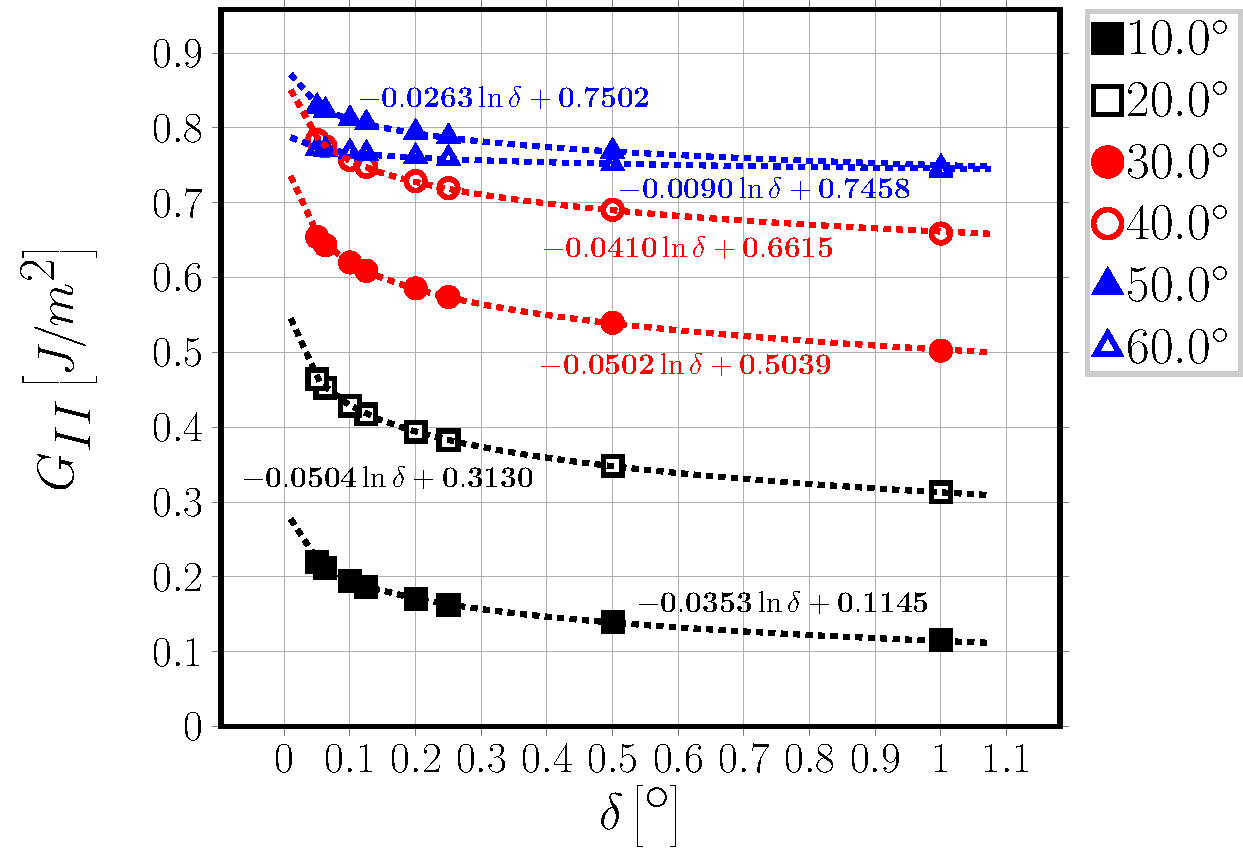
\includegraphics[width=\textwidth]{Vf40-free-2nd-vsDelta-GII.pdf}
       \caption{$2^{nd}$ order elements.}
    \end{subfigure}
    ~
    \begin{subfigure}[b]{0.48\textwidth}
        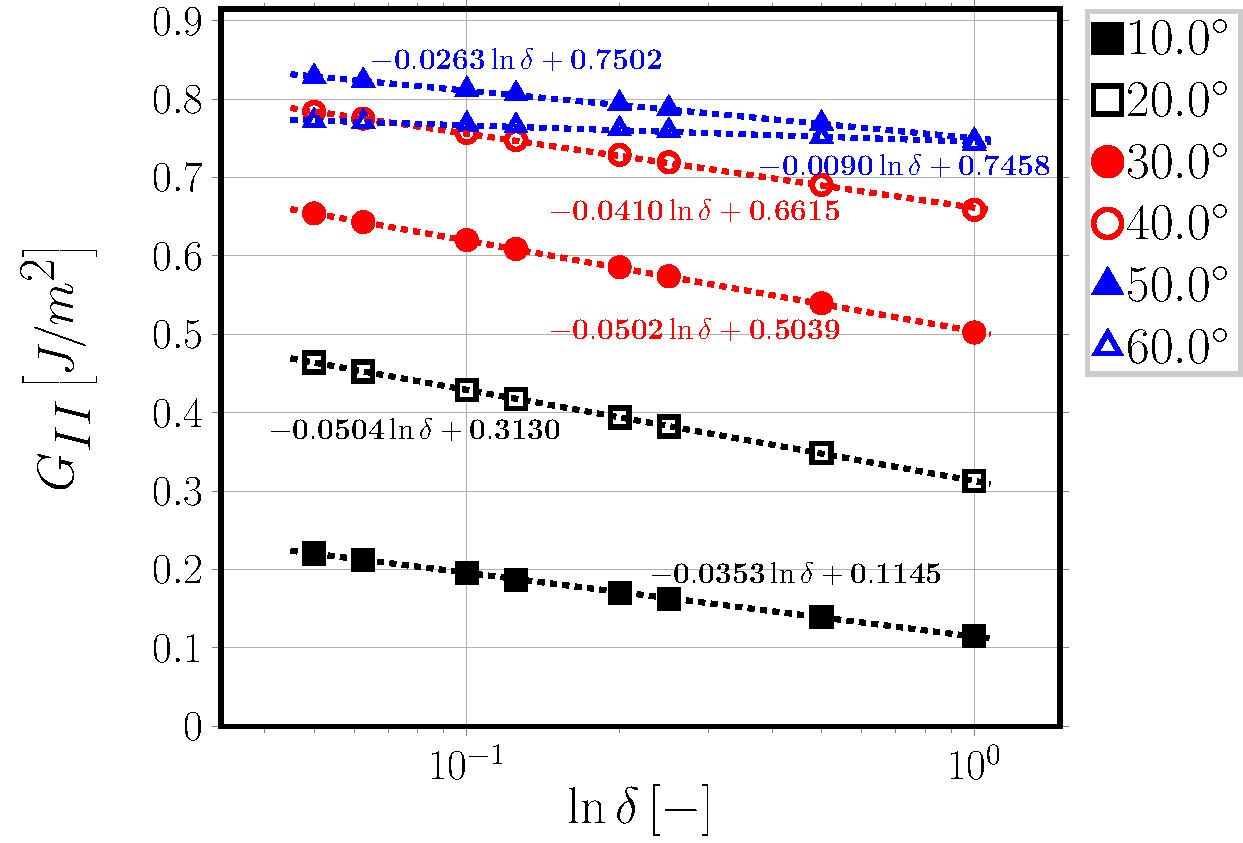
\includegraphics[width=\textwidth]{Vf40-free-2nd-semilogvsDelta-GII.pdf}
       \caption{$2^{nd}$ order elements.}
    \end{subfigure}

\caption{Logarithmic dependence on $\delta$ of Mode II ERR: interpolation of numerical results for $V_{f}=40\%$.}\label{fig:giiinterp40}
\end{figure}

As shown in Fig.~\ref{fig:giinterp01}, Fig.~\ref{fig:giinterp40}, Fig.~\ref{fig:giiinterp01} and Fig.~\ref{fig:giiinterp40} both in linear and logarithmic scales of $\delta$, the result is remarkable: both the correlation coefficient $r$ and the $r^{2}$ ratio (of explained to total variance) are always greater than $0.95$ and the $p$-values of the coefficients $A$ and $B$ are at least $<1E-6$ and often $<1E-11$ (see Table~\ref{tab:GIinterp} for $G_{I}$ and Table~\ref{tab:GIIinterp} for $G_{II}$). The results of the linear regression confirm the analytical derivations of the previous section, which showed the logarithmic behavior of Mode I and Mode II ERR. Similar conclusions were reached in~\cite{Sun1987,Manoharan1990} for a straight bi-material crack with respect to the parameter $\nicefrac{\Delta a}{a}$; however, no functional expression of $G_{\left(\cdot\right)}$ was proposed.

\section{Conclusions \& Outlook}

The application of the Virtual Crack Closure Technique to the calculation of Mode I, Mode II and total Energy Release Rate was analyzed in the context of the Finite Element solution of the bi-material circular arc crack, or fiber-matrix interface crack. A synthetic vectorial formulation of the VCCT has been proposed and its usefulness exemplified in the analysis of the mesh dependency. By both analytical considerations and numerical simulations, it has been shown that:

\begin{itemize}
\item the total ERR is invariant to rotations of the reference frame (and more in general to linear transformations), which implies that rotation of crack tip forces and displacement is actually not required in the use of the VCCT for the calculation of $G_{TOT}$;
\item the total ERR does not depend on the size $\delta$ of the elements at the crack tip, at least for reasonably small elements ($\delta\leq1.0^{\circ}$) ;
\item as a consequence, Mode II ERR for the \emph{closed} interface crack does not depend on $\delta$, as $G_{II}=G_{TOT}$ after the onset of the contact zone;
\item for the \emph{open} interface crack, Mode I and Mode II ERR depend on the element size $\delta$ through a logarithmic law of the type $A\left(\Delta\theta\right)\ln\delta+B\left(\Delta\theta\right)$;
\item the sign of the logarithm is always positive for $G_{I}$, i.e. it decreases when $\delta$ decreases, and negative for $G_{II}$, i.e. it increases when $\delta$ decreases.
\end{itemize}

The conclusion is significant: as the behavior of Mode I and Mode II is logarithmic with respect to mesh size, there exists no asymptotic limit and thus no convergence of the values. A convergence analysis based on the reduction of the error between successive iterations would not provide a reliable assessment of the accuracy of the FE solution of Mode I and Mode II Energy Release Rate of the fiber-matrix interface crack. A validation is thus required with respect to data obtained through a different method, be it analytical, numerical or experimental. Moreover, it has been shown that: first, the same behavior appears when using $1^{st}$ as well as $2^{nd}$ order elements; second, no improvement is expected with the use of singular elements, as the logarithmic dependency of $G_{I}$ and $G_{II}$ is governed by the definition of ERR itself together with the asymptotic behavior of the displacement field at the crack tip. These two conclusions run contrary to the suggestions provided in the manuals of many commercial FEM packages, such as Abaqus~\cite{abq12} which suggests that (Section 11.4.2 of the \emph{Abaqus Analysis User's Guide}): ``\textit{Sharp cracks (where the crack faces lie on top of one another in the undeformed configuration) are usually modeled using small-strain assumptions. Focused meshes, [...], should normally be used for small-strain fracture mechanics evaluations. However, for a sharp crack the strain field becomes singular at the crack tip. [...] In most cases the singularity at the crack tip should be considered in small-strain analysis (when geometric nonlinearities are ignored). Including the singularity often improves the accuracy of the J-integral, the stress intensity factors, and the stress and strain calculations because the stresses and strains in the region close to the crack tip are more accurate.}''. We have shown that, in the context of the fiber/matrix interface crack, the convergence of the Energy Release Rate is determined by the asymptotic behavior of the elastic solution and only marginally by the choice of element order and type, thus contradicting the statements in~\cite{abq12}. 

\FloatBarrier

\section*{Acknowledgements}

Luca Di Stasio thanks Prof. Janis Varna for the useful discussions and suggestions. Luca Di Stasio gratefully acknowledges the support of the European School of Materials (EUSMAT) through the DocMASE Doctoral Programme and the European Commission through the Erasmus Mundus Programme.

\bibliography{refs}

\appendix
\section{Derivation of the relationship between crack tip forces and displacements for first order quadrilateral elements}\label{app:ctforcesexample}

\subsection{Foundational relations}

In the isoparametric formulation of the Finite Element Method, the element Jacobian $J$ and its inverse $J^{-1}$ can be expressed in general as 

\begin{equation}
\underline{\underline{J}}=\begin{bmatrix}
\underline{e}_{\xi}|\underline{e}_{\eta}
\end{bmatrix}=\begin{bmatrix}
\frac{\partial x}{\partial\xi}&\frac{\partial x}{\partial\eta}\\\frac{\partial y}{\partial\xi}&\frac{\partial y}{\partial\eta}
\end{bmatrix}\qquad\underline{\underline{J}}^{-1}=\begin{bmatrix}
\underline{e}^{x}|\underline{e}^{y}
\end{bmatrix}=\begin{bmatrix}
\frac{\partial \xi}{\partial x}&\frac{\partial \xi}{\partial y}\\\frac{\partial \eta}{\partial x}&\frac{\partial \eta}{\partial y}
\end{bmatrix}
\end{equation}

where $\left\{e_{\xi}, e_{\eta}\right\}$ and $\left\{e^{x}, e^{y}\right\}$ are respectively the covariant and contravariant basis vectors of the mapping between global $\left\{x, y\right\}$ and local element $\left\{\xi, \eta\right\}$ coordinates:

\begin{equation}
\underline{e}_{\xi}=\begin{bmatrix}
\frac{\partial x}{\partial\xi}\\\frac{\partial y}{\partial\xi}
\end{bmatrix}\quad\underline{e}_{\eta}=\begin{bmatrix}
\frac{\partial x}{\partial\eta}\\\frac{\partial y}{\partial\eta}
\end{bmatrix},
\end{equation}

\begin{equation}
\underline{e}_{x}=\begin{bmatrix}
\frac{\partial \xi}{\partial x}\\\frac{\partial \eta}{\partial x}
\end{bmatrix}\quad\underline{e}_{y}=\begin{bmatrix}
\frac{\partial \xi}{\partial y}\\\frac{\partial \eta}{\partial y}
\end{bmatrix}.
\end{equation}

Denoting by $d$ the number of geometrical dimensions of the problem ($d=2$ in the present work) and by $\underline{p}$ the $d\times 1$ position vector in global coordinates, we can formally introduce the $3\left(d-1\right)\times d$ matrix operator of partial differentiation $\underline{\underline{\widetilde{B}}}$ such that

\begin{equation}\label{eq:introB}
\underline{\varepsilon}\left(\underline{p}\right)=\underline{\underline{\widetilde{B}}}\cdot\underline{u}\left(\underline{p}\right),
\end{equation}

where $\underline{u}$ and $\underline{\varepsilon}$ are respectively the $d\times 1$ displacement vector and the $3\left(d-1\right)\times 1$ strain vector in Voigt notation. Denoting by $n$ the number of nodes of a generic element ($n=s\times m$ where $s$ represents the number of sides of the element and $m$ the order of the shape functions), we can furthermore introduce the $d\times d\cdot n$ matrix \underline{\underline{N}} of shape functions such that

\begin{equation}\label{eq:introN}
\underline{u}=\underline{\underline{N}}\cdot\underline{u}_{N},
\end{equation}

where $\underline{u}_{N}$ is the $d\cdot n\times 1$ vector of element nodal variables. Having introduced $\underline{\underline{\widetilde{B}}}$ and $\underline{\underline{N}}$ in Equations~\ref{eq:introB} and~\ref{eq:introN} respectively, it is possible to define the $3\left(d-1\right)\times d\cdot n$ matrix $\underline{\underline{B}}$ of derivatives (with respect to global coordinates) of shape functions as

\begin{equation}
\underline{\underline{B}}=\underline{\underline{\widetilde{B}}}\cdot\underline{\underline{N}}.
\end{equation}

We introduce the linear elastic material behavior in the form of the $3\left(d-1\right)\times 3\left(d-1\right)$ rigidity matrix $\underline{\underline{D}}$ such that

\begin{equation}
\underline{\sigma}=\underline{\underline{D}}\cdot\underline{\varepsilon},
\end{equation}

where $\underline{\sigma}$ the $3\left(d-1\right)\times 1$ stress vector in Voigt notation. It is finally possible to define the $n\times n$ element stiffness matrix $\underline{\underline{k_{e}}}$ as 

\begin{equation}\label{eq:elestiff}
\underline{\underline{k_{e}}}=\int_{V_{e}\left(x,y\right)}\left(\underline{\underline{B}}^{T}\underline{\underline{D}}\cdot\underline{\underline{B}}\right)dV_{e}\left(x,\dots,y\right)=\int_{V_{e}\left(\xi,\eta\right)}\left(\underline{\underline{B}}^{T}\underline{\underline{D}}\cdot\underline{\underline{B}}\right)\sqrt{g}dV_{e}\left(\xi,\dots,\eta\right),
\end{equation}

where $g=det\left(\underline{\underline{J}}^{T}\underline{\underline{J}}\right)$ and $V_{e}$ is the element volume. Given that isoparametric elements are always defined between $-1$ and $1$ in each dimension, Equation~\ref{eq:elestiff} can simplified to

\begin{equation}
\underline{\underline{k_{e}}}=\int_{-1}^{1}\dots\int_{-1}^{1}\left(\underline{\underline{B}}^{T}\underline{\underline{D}}\cdot\underline{\underline{B}}\right)\sqrt{g}d\xi,\dots, d\eta,
\end{equation}

which is amenable to numerical integration by means of a Gaussian quadrature of the form

\begin{equation}\label{eq:elstiffnum}
\underline{\underline{k_{e}}}\approx \sum_{i=1}^{N}\dots\sum_{j=1}^{N}w_{i}\dots w_{j}\left(\underline{\underline{B}}^{T}\left(\xi_{i}, \dots,\eta_{j}\right)\cdot\underline{\underline{D}}\cdot\underline{\underline{B}}\left(\xi_{i}, \dots,\eta_{j}\right)\sqrt{g}\right),
\end{equation}

where $\left(\xi_{i}, \dots,\eta_{j}\right)$ are the coordinates of the $N$ Gaussian quadrature points. The element stiffness matrix as evaluated in Eq.~\ref{eq:elstiffnum} is in general a full symmetric (in the case of linear elasticity) matrix of the form

\begin{equation}\label{eq:elstiffmatrix}
k_{e}=\begin{bmatrix}
k_{e|11}&k_{e|12}&k_{e|13}&k_{e|14}&k_{e|15}&k_{e|16}&k_{e|17}&k_{e|18}\\
k_{e|12}&k_{e|22}&k_{e|23}&k_{e|24}&k_{e|25}&k_{e|26}&k_{e|27}&k_{e|28}\\
k_{e|13}&k_{e|23}&k_{e|33}&k_{e|34}&k_{e|35}&k_{e|36}&k_{e|37}&k_{e|38}\\
k_{e|14}&k_{e|24}&k_{e|34}&k_{e|44}&k_{e|45}&k_{e|46}&k_{e|47}&k_{e|48}\\
k_{e|15}&k_{e|25}&k_{e|35}&k_{e|45}&k_{e|55}&k_{e|56}&k_{e|57}&k_{e|58}\\
k_{e|16}&k_{e|26}&k_{e|36}&k_{e|46}&k_{e|56}&k_{e|66}&k_{e|67}&k_{e|68}\\
k_{e|17}&k_{e|27}&k_{e|37}&k_{e|47}&k_{e|57}&k_{e|67}&k_{e|77}&k_{e|78}\\
k_{e|18}&k_{e|28}&k_{e|38}&k_{e|48}&k_{e|58}&k_{e|68}&k_{e|78}&k_{e|88}\\
\end{bmatrix}.
\end{equation}

\subsection{Calculation of displacements and reaction forces}

With reference to Fig.~\ref{fig:vcctlinear}, we define:

\begin{description}
\item[$u_{x,M}$, $u_{x,F}$] the $x$-displacement of the nodes belonging to the free side of the first element belonging to the crack, respectively on the matrix (bulk) and fiber (inclusion) side;
\item[$u_{y,M}$, $u_{y,F}$] the $y$-displacement of the nodes belonging to the free side of the first element belonging to the crack, respectively on the matrix (bulk) and fiber (inclusion) side;
\item[$u_{r,M}$, $u_{r,F}$] the $x$-displacement of the nodes belonging to the free side of the first element belonging to the crack, respectively on the matrix (bulk) and fiber (inclusion) side;
\item[$u_{\theta,M}$, $u_{\theta,F}$] the $y$-displacement of the nodes belonging to the free side of the first element belonging to the crack, respectively on the matrix (bulk) and fiber (inclusion) side;
\item[$F_{x,CT}$, $F_{y,CT}$] respectively the $x$- and $y$-component of the reaction force at the crack tip;
\item[$F_{r,CT}$, $F_{\theta,CT}$] respectively the $r$- and $\theta$-component of the reaction force at the crack tip.
\end{description}

The $x-y$ reference frame is the global reference frame, while the $r-\theta$ reference frame is such that the $\theta$ direction coincides with the crack propagation direction at the crack tip and $r$ the in-plane normal to the propagation direction. For an arc-crack as the present one, the $r$-direction coincides with the radial direction of the inclusion.

\begin{figure}[!h]
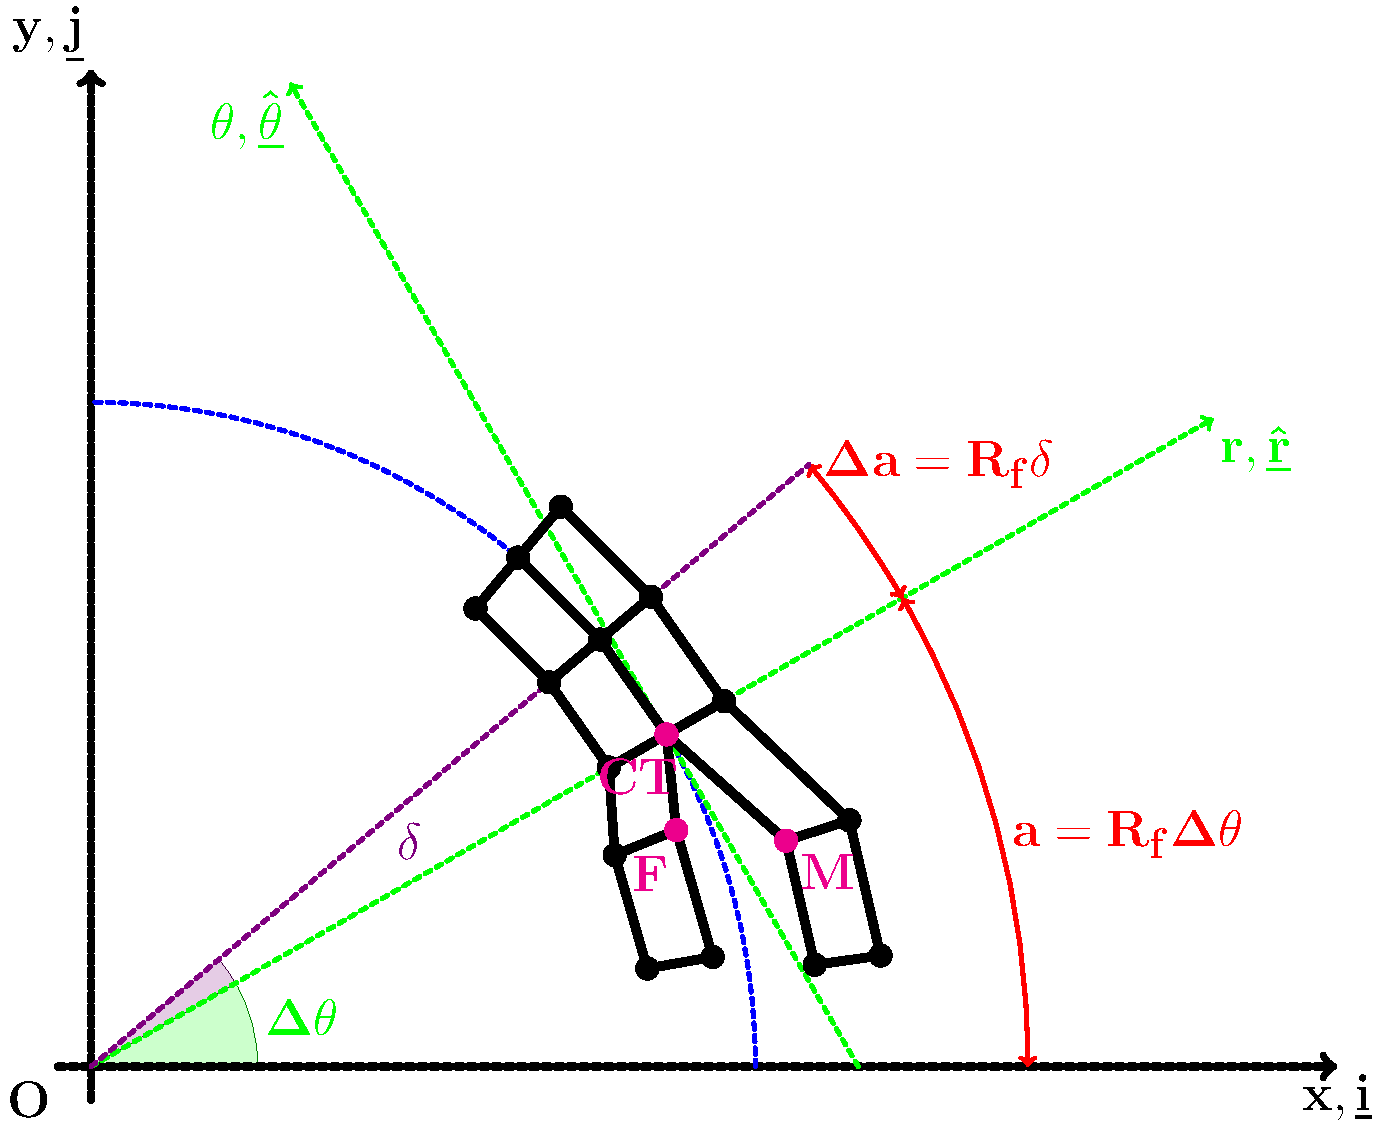
\includegraphics[width=\textwidth]{VCCT-linear.pdf}
\caption{Schematic representation of the discretized crack tip geometry for  $1^{st}$ order quadrilateral elements.}\label{fig:vcctlinear}
\end{figure}

The crack opening displacement $u_{r}$ and the crack shear displacement $u_{\theta}$ at the crack tip can thus be written as

\begin{equation}
u_{r}=\cos\left(\Delta\theta\right) u_{x}+\sin\left(\Delta\theta\right) u_{y}\qquad u_{\theta}=-\sin\left(\Delta\theta\right) u_{x}+\cos\left(\Delta\theta\right) u_{y},
\end{equation}

where $u_{x}$ and $u_{y}$ are defined as

\begin{equation}\label{eq:uxuy}
u_{x}=u_{x,M}-u_{x,F}\qquad u_{y}=u_{y,M}-u_{y,F}
\end{equation}

and $2\Delta\theta$ is total angular size of the debond. The corresponding forces at the crack tip are

\begin{equation}
F_{r}=\cos\left(\Delta\theta\right) F_{x,CT}+\sin\left(\Delta\theta\right) F_{y,CT}\qquad F_{\theta}=-\sin\left(\Delta\theta\right) F_{x,CT}+\cos\left(\Delta\theta\right) F_{y,CT}.
\end{equation}

At the crack tip, the FE mesh possesses two coincident points, labeled $FCT$ and $MCT$. Continuity of the displacements at the crack tip must be ensured. Furthermore, in order to measure the force at the crack tip, a fully-constraint dummy node needs to be created and formally linked to the two nodes at the crack tip by the conditions 

\begin{equation}
\begin{cases}
&u_{x,FCT}-u_{x,MCT}-u_{x,DUMMY}=0\\
&u_{y,FCT}-u_{y,MCT}-u_{y,DUMMY}=0\\[10pt]
&u_{x,DUMMY}=0\\
&u_{y,DUMMY}=0\\
\end{cases},
\end{equation}

which can be simplified to

\begin{equation}
\begin{cases}
&u_{x,FCT}=u_{x,MCT}\\
&u_{y,FCT}=u_{y,MCT}\\[10pt]
&R_{x,DUMMY}=R_{x,FCT}=-R_{x,MCT}=F_{x,CT}\\
&R_{y,DUMMY}=R_{y,FCT}=-R_{y,MCT}=F_{y,CT}\\
\end{cases}.
\end{equation}

Making use of Eq.~\ref{eq:elstiffmatrix}, four equations can be written in the four displacement $u_{x,FCT}$, $u_{x,MCT}$, $u_{y,FCT}$ and $u_{y,MCT}$:

\begin{equation}\label{eq:syseqs01}
\begin{cases}
&\left(k_{e,M|11}+k_{e,M|33}\right)u_{x,MCT}+\left(k_{e,M|12}+k_{e,M|34}\right)u_{y,MCT}+\\&+k_{e,M|13}u_{x,M}+k_{e,M|14}u_{y,M}+\left(k_{M|17}+k_{M|35}\right)u_{N,MC|7}+\left(k_{M|18}+k_{M|36}\right)u_{N,MC|8}+\\&+\sum_{i=5}^{6}k_{M|1i}u_{N,MC|i}+\sum_{i=7}^{8}k_{M|3i}u_{N,MB|i}+k_{M|31}u_{x,NCOI}+k_{M|32}u_{y,NCOI}=0\\[10pt]
&\left(k_{e,M|21}+k_{e,M|43}\right)u_{x,MCT}+\left(k_{e,M|22}+k_{e,M|44}\right)u_{y,MCT}+\\&+k_{e,M|23}u_{x,M}+k_{e,M|24}u_{y,M}+\left(k_{M|27}+k_{M|45}\right)u_{N,MC|7}+\left(k_{M|28}+k_{M|46}\right)u_{N,MC|8}+\\&+\sum_{i=5}^{6}k_{M|2i}u_{N,MC|i}+\sum_{i=7}^{8}k_{M|4i}u_{N,MB|i}+k_{M|41}u_{x,NCOI}+k_{M|42}u_{y,NCOI}=0\\[10pt]
&\left(k_{e,F|77}+k_{e,F|55}\right)u_{x,FCT}+\left(k_{e,F|78}+k_{e,F|56}\right)u_{y,FCT}+\\&+k_{e,F|75}u_{x,F}+k_{e,F|76}u_{y,F}+\left(k_{F|71}+k_{F|53}\right)u_{N,FC|1}+\left(k_{F|72}+k_{F|54}\right)u_{N,FC|2}+\\&+\sum_{i=2}^{3}k_{F|7i}u_{N,FC|i}+\sum_{i=1}^{2}k_{F|5i}u_{N,FB|i}+k_{F|57}u_{x,NCOI}+k_{F|58}u_{y,NCOI}=0\\[10pt]
&\left(k_{e,F|87}+k_{e,F|65}\right)u_{x,FCT}+\left(k_{e,F|88}+k_{e,F|66}\right)u_{y,FCT}+\\&+k_{e,F|85}u_{x,F}+k_{e,F|86}u_{y,F}+\left(k_{F|81}+k_{F|63}\right)u_{N,FC|1}+\left(k_{F|82}+k_{F|64}\right)u_{N,FC|2}+\\&+\sum_{i=2}^{3}k_{F|8i}u_{N,FC|i}+\sum_{i=1}^{2}k_{F|6i}u_{N,FB|i}+k_{F|67}u_{x,NCOI}+k_{F|68}u_{y,NCOI}=0\\[10pt]
\end{cases}.
\end{equation}

Solving for $u_{y,FCT}$ and $u_{y,MCT}$ the third and fourth relations in Eq.~\ref{eq:syseqs01} and substituting in the first two expressions of Eq.~\ref{eq:syseqs01}, we get

\begin{equation}\label{eq:syseqs02}
\footnotesize
\begin{cases}
&\left(k_{e,M|11}+k_{e,M|33}+k_{e,F|77}+k_{e,F|55}\right)u_{x,MCT}+\left(k_{e,M|12}+k_{e,M|34}+k_{e,F|78}+k_{e,F|56}\right)u_{y,MCT}+\\&+k_{e,M|13}u_{x,M}+k_{e,M|14}u_{y,M}+k_{e,F|75}u_{x,F}+k_{e,F|76}u_{y,F}+\\&+\left(k_{M|31}+k_{F|57}\right)u_{x,NCOI}+\left(k_{M|32}+k_{F|58}\right)u_{y,NCOI}+\\&+\left(k_{M|17}+k_{M|35}\right)u_{N,MC|7}+\left(k_{M|18}+k_{M|36}\right)u_{N,MC|8}+\left(k_{F|71}+k_{F|53}\right)u_{N,FC|1}+\left(k_{F|72}+k_{F|54}\right)u_{N,FC|2}+\\&+\sum_{i=5}^{6}k_{M|1i}u_{N,MC|i}+\sum_{i=7}^{8}k_{M|3i}u_{N,MB|i}+\sum_{i=2}^{3}k_{F|7i}u_{N,FC|i}+\sum_{i=1}^{2}k_{F|5i}u_{N,FB|i}=0\\[10pt]
&\left(k_{e,M|21}+k_{e,M|43}+k_{e,F|87}+k_{e,F|65}\right)u_{x,MCT}+\left(k_{e,M|22}+k_{e,M|44}+k_{e,F|88}+k_{e,F|66}\right)u_{y,MCT}+\\&+k_{e,M|23}u_{x,M}+k_{e,M|24}u_{y,M}+k_{e,F|85}u_{x,F}+k_{e,F|86}u_{y,F}+\\&+\left(k_{M|41}+k_{F|67}\right)u_{x,NCOI}+\left(k_{M|42}+k_{F|68}\right)u_{y,NCOI}+\\&+\left(k_{M|27}+k_{M|45}\right)u_{N,MC|7}+\left(k_{M|28}+k_{M|46}\right)u_{N,MC|8}+\left(k_{F|81}+k_{F|63}\right)u_{N,FC|1}+\left(k_{F|82}+k_{F|64}\right)u_{N,FC|2}+\\&+\sum_{i=2}^{3}k_{F|8i}u_{N,FC|i}+\sum_{i=1}^{2}k_{F|6i}u_{N,FB|i}+\sum_{i=5}^{6}k_{M|2i}u_{N,MC|i}+\sum_{i=7}^{8}k_{M|4i}u_{N,MB|i}=0\\[10pt]
\end{cases}
\end{equation}

%\begin{equation}
%\scriptsize
%\begin{cases}
%&u_{y,MCT}=-\frac{k_{e,M|11}+k_{e,M|33}+k_{e,F|77}+k_{e,F|55}}{k_{e,M|12}+k_{e,M|34}+k_{e,F|78}+k_{e,F|56}}u_{x,MCT}+\\
%&-\frac{k_{e,M|13}u_{x,M}+k_{e,M|14}u_{y,M}+k_{e,F|75}u_{x,F}+k_{e,F|76}u_{y,F}}{k_{e,M|12}+k_{e,M|34}+k_{e,F|78}+k_{e,F|56}}+\\
%&-\frac{\left(k_{M|31}+k_{F|57}\right)u_{x,NCOI}+\left(k_{M|32}+k_{F|58}\right)u_{y,NCOI}}{k_{e,M|12}+k_{e,M|34}+k_{e,F|78}+k_{e,F|56}}+\\
%&-\frac{\left(k_{M|17}+k_{M|35}\right)u_{N,MC|7}+\left(k_{M|18}+k_{M|36}\right)u_{N,MC|8}+\left(k_{F|71}+k_{F|53}\right)u_{N,FC|1}+\left(k_{F|72}+k_{F|54}\right)u_{N,FC|2}}{k_{e,M|12}+k_{e,M|34}+k_{e,F|78}+k_{e,F|56}}+\\
%&-\frac{\sum_{i=5}^{6}k_{M|1i}u_{N,MC|i}+\sum_{i=7}^{8}k_{M|3i}u_{N,MB|i}+\sum_{i=2}^{3}k_{F|7i}u_{N,FC|i}+\sum_{i=1}^{2}k_{F|5i}u_{N,FB|i}}{k_{e,M|12}+k_{e,M|34}+k_{e,F|78}+k_{e,F|56}}\\[10pt]
%
%&\left[\left(k_{e,M|21}+k_{e,M|43}+k_{e,F|87}+k_{e,F|65}\right)+\frac{k_{e,M|11}+k_{e,M|33}+k_{e,F|77}+k_{e,F|55}}{k_{e,M|12}+k_{e,M|34}+k_{e,F|78}+k_{e,F|56}}\left(k_{e,M|22}+k_{e,M|44}+k_{e,F|88}+k_{e,F|66}\right)\right]u_{x,MCT}+\\
%&+\left(k_{e,M|23}-\frac{k_{e,M|22}+k_{e,M|44}+k_{e,F|88}+k_{e,F|66}}{k_{e,M|12}+k_{e,M|34}+k_{e,F|78}+k_{e,F|56}}k_{e,M|13}\right)u_{x,M}+\\
%&+\left(k_{e,M|24}-\frac{k_{e,M|22}+k_{e,M|44}+k_{e,F|88}+k_{e,F|66}}{k_{e,M|12}+k_{e,M|34}+k_{e,F|78}+k_{e,F|56}}k_{e,M|14}\right)u_{y,M}+\\
%&+\left(k_{e,F|85}-\frac{k_{e,M|22}+k_{e,M|44}+k_{e,F|88}+k_{e,F|66}}{k_{e,M|12}+k_{e,M|34}+k_{e,F|78}+k_{e,F|56}}k_{e,M|75}\right)u_{x,F}+\\
%&+\left(k_{e,F|86}-\frac{k_{e,M|22}+k_{e,M|44}+k_{e,F|88}+k_{e,F|66}}{k_{e,M|12}+k_{e,M|34}+k_{e,F|78}+k_{e,F|56}}k_{e,M|76}\right)u_{y,F}+\\
%&+\left[\left(k_{M|41}+k_{F|67}\right)-\frac{k_{e,M|22}+k_{e,M|44}+k_{e,F|88}+k_{e,F|66}}{k_{e,M|12}+k_{e,M|34}+k_{e,F|78}+k_{e,F|56}}\left(k_{M|31}+k_{F|57}\right)\right]u_{x,NCOI}+\\
%&+\left[\left(k_{M|42}+k_{F|68}\right)-\frac{k_{e,M|22}+k_{e,M|44}+k_{e,F|88}+k_{e,F|66}}{k_{e,M|12}+k_{e,M|34}+k_{e,F|78}+k_{e,F|56}}\left(k_{M|32}+k_{F|58}\right)\right]u_{y,NCOI}+\\
%&+\left(k_{M|27}+k_{M|45}\right)u_{N,MC|7}+\left(k_{M|28}+k_{M|46}\right)u_{N,MC|8}+\left(k_{F|81}+k_{F|63}\right)u_{N,FC|1}+\left(k_{F|82}+k_{F|64}\right)u_{N,FC|2}+\\
%&-\frac{k_{e,M|22}+k_{e,M|44}+k_{e,F|88}+k_{e,F|66}}{k_{e,M|12}+k_{e,M|34}+k_{e,F|78}+k_{e,F|56}}\left[\left(k_{M|17}+k_{M|35}\right)u_{N,MC|7}+\left(k_{M|18}+k_{M|36}\right)u_{N,MC|8}\right]+\\&
%-\frac{k_{e,M|22}+k_{e,M|44}+k_{e,F|88}+k_{e,F|66}}{k_{e,M|12}+k_{e,M|34}+k_{e,F|78}+k_{e,F|56}}\left[\left(k_{F|71}+k_{F|53}\right)u_{N,FC|1}+\left(k_{F|72}+k_{F|54}\right)u_{N,FC|2}\right]\\
%&+\sum_{i=2}^{3}k_{F|8i}u_{N,FC|i}+\sum_{i=1}^{2}k_{F|6i}u_{N,FB|i}+\sum_{i=5}^{6}k_{M|2i}u_{N,MC|i}+\sum_{i=7}^{8}k_{M|4i}u_{N,MB|i}+\\
%&-\frac{\sum_{i=5}^{6}k_{M|1i}u_{N,MC|i}+\sum_{i=7}^{8}k_{M|3i}u_{N,MB|i}+\sum_{i=2}^{3}k_{F|7i}u_{N,FC|i}+\sum_{i=1}^{2}k_{F|5i}u_{N,FB|i}}{k_{e,M|12}+k_{e,M|34}+k_{e,F|78}+k_{e,F|56}}=0\\[10pt]
%
%&u_{x,FCT}=u_{x,MCT}\\
%&u_{y,FCT}=u_{y,MCT}\\[10pt]
%&R_{x,DUMMY}=R_{x,FCT}=-R_{x,MCT}=F_{x,CT}\\
%&R_{y,DUMMY}=R_{y,FCT}=-R_{y,MCT}=F_{y,CT}\\
%\end{cases}
%\end{equation}

Solving the system of two equations and observing that $u_{x,F},u_{y,F}\sim0$ for a stiffer inclusion as a fiber in a polymeric composite, we can express $u_{x,MCT}$ as a function of $u_{x}$ and $u_{y}$ (see Eq.~\ref{eq:uxuy}) as

\begin{equation}\label{eq:syseqs03}
\scriptsize
\begin{split}
%&u_{y,MCT}=-\frac{k_{e,M|11}+k_{e,M|33}+k_{e,F|77}+k_{e,F|55}}{k_{e,M|12}+k_{e,M|34}+k_{e,F|78}+k_{e,F|56}}u_{x,MCT}+\\
%&-\frac{k_{e,M|13}u_{x,M}+k_{e,M|14}u_{y,M}+k_{e,F|75}u_{x,F}+k_{e,F|76}u_{y,F}}{k_{e,M|12}+k_{e,M|34}+k_{e,F|78}+k_{e,F|56}}+\\
%&-\frac{\left(k_{M|31}+k_{F|57}\right)u_{x,NCOI}+\left(k_{M|32}+k_{F|58}\right)u_{y,NCOI}}{k_{e,M|12}+k_{e,M|34}+k_{e,F|78}+k_{e,F|56}}+\\
%&-\frac{\left(k_{M|17}+k_{M|35}\right)u_{N,MC|7}+\left(k_{M|18}+k_{M|36}\right)u_{N,MC|8}+\left(k_{F|71}+k_{F|53}\right)u_{N,FC|1}+\left(k_{F|72}+k_{F|54}\right)u_{N,FC|2}}{k_{e,M|12}+k_{e,M|34}+k_{e,F|78}+k_{e,F|56}}+\\
%&-\frac{\sum_{i=5}^{6}k_{M|1i}u_{N,MC|i}+\sum_{i=7}^{8}k_{M|3i}u_{N,MB|i}+\sum_{i=2}^{3}k_{F|7i}u_{N,FC|i}+\sum_{i=1}^{2}k_{F|5i}u_{N,FB|i}}{k_{e,M|12}+k_{e,M|34}+k_{e,F|78}+k_{e,F|56}}\\[10pt]
&\left[\left(k_{e,M|21}+k_{e,M|43}+k_{e,F|87}+k_{e,F|65}\right)+\frac{k_{e,M|11}+k_{e,M|33}+k_{e,F|77}+k_{e,F|55}}{k_{e,M|12}+k_{e,M|34}+k_{e,F|78}+k_{e,F|56}}\left(k_{e,M|22}+k_{e,M|44}+k_{e,F|88}+k_{e,F|66}\right)\right]u_{x,MCT}+\\
&+\left(k_{e,M|23}-\frac{k_{e,M|22}+k_{e,M|44}+k_{e,F|88}+k_{e,F|66}}{k_{e,M|12}+k_{e,M|34}+k_{e,F|78}+k_{e,F|56}}k_{e,M|13}\right)u_{x}+\\
&+\left(k_{e,M|24}-\frac{k_{e,M|22}+k_{e,M|44}+k_{e,F|88}+k_{e,F|66}}{k_{e,M|12}+k_{e,M|34}+k_{e,F|78}+k_{e,F|56}}k_{e,M|14}\right)u_{y}+\\
&+\left(k_{e,M|23}+k_{e,F|85}-\frac{k_{e,M|22}+k_{e,M|44}+k_{e,F|88}+k_{e,F|66}}{k_{e,M|12}+k_{e,M|34}+k_{e,F|78}+k_{e,F|56}}\left(k_{e,M|13}+k_{e,M|75}\right)\right)\cancelto{\approx 0}{u_{x,F}}+\\
&+\left(k_{e,M|24}+k_{e,F|86}-\frac{k_{e,M|22}+k_{e,M|44}+k_{e,F|88}+k_{e,F|66}}{k_{e,M|12}+k_{e,M|34}+k_{e,F|78}+k_{e,F|56}}\left(k_{e,M|14}+k_{e,M|76}\right)\right)\cancelto{\approx 0}{u_{y,F}}+\\
&+\left[\left(k_{M|41}+k_{F|67}\right)-\frac{k_{e,M|22}+k_{e,M|44}+k_{e,F|88}+k_{e,F|66}}{k_{e,M|12}+k_{e,M|34}+k_{e,F|78}+k_{e,F|56}}\left(k_{M|31}+k_{F|57}\right)\right]u_{x,NCOI}+\\
&+\left[\left(k_{M|42}+k_{F|68}\right)-\frac{k_{e,M|22}+k_{e,M|44}+k_{e,F|88}+k_{e,F|66}}{k_{e,M|12}+k_{e,M|34}+k_{e,F|78}+k_{e,F|56}}\left(k_{M|32}+k_{F|58}\right)\right]u_{y,NCOI}+\\
&+\left(k_{M|27}+k_{M|45}\right)u_{N,MC|7}+\left(k_{M|28}+k_{M|46}\right)u_{N,MC|8}+\left(k_{F|81}+k_{F|63}\right)u_{N,FC|1}+\left(k_{F|82}+k_{F|64}\right)u_{N,FC|2}+\\
&-\frac{k_{e,M|22}+k_{e,M|44}+k_{e,F|88}+k_{e,F|66}}{k_{e,M|12}+k_{e,M|34}+k_{e,F|78}+k_{e,F|56}}\left[\left(k_{M|17}+k_{M|35}\right)u_{N,MC|7}+\left(k_{M|18}+k_{M|36}\right)u_{N,MC|8}\right]+\\&
-\frac{k_{e,M|22}+k_{e,M|44}+k_{e,F|88}+k_{e,F|66}}{k_{e,M|12}+k_{e,M|34}+k_{e,F|78}+k_{e,F|56}}\left[\left(k_{F|71}+k_{F|53}\right)u_{N,FC|1}+\left(k_{F|72}+k_{F|54}\right)u_{N,FC|2}\right]\\
&+\sum_{i=2}^{3}k_{F|8i}u_{N,FC|i}+\sum_{i=1}^{2}k_{F|6i}u_{N,FB|i}+\sum_{i=5}^{6}k_{M|2i}u_{N,MC|i}+\sum_{i=7}^{8}k_{M|4i}u_{N,MB|i}+\\
&-\frac{\sum_{i=5}^{6}k_{M|1i}u_{N,MC|i}+\sum_{i=7}^{8}k_{M|3i}u_{N,MB|i}+\sum_{i=2}^{3}k_{F|7i}u_{N,FC|i}+\sum_{i=1}^{2}k_{F|5i}u_{N,FB|i}}{k_{e,M|12}+k_{e,M|34}+k_{e,F|78}+k_{e,F|56}}=0,
\end{split}
\end{equation}

while the reaction forces at the crack tip can be expressed as

\begin{equation}\label{eq:forcesreform}
\begin{cases}
F_{x,CT}&=R_{x,FCT}=\\&=\left(k_{e,F|77}+k_{e,F|55}\right)u_{x,FCT}+\left(k_{e,F|78}+k_{e,F|56}\right)u_{y,FCT}+\\
&+k_{e,F|75}\cancelto{\approx 0}{u_{x,F}}+k_{e,F|76}\cancelto{\approx 0}{u_{y,F}}+\\
&+\sum_{i=1}^{4}k_{e,F|7i}u_{N,FC|i}+\sum_{i=1,i\neq\left(5,6\right)}^{8}k_{e,F|5i}u_{N,FB|i}\\
F_{y,CT}&=R_{y,FCT}=\\&=\left(k_{e,F|87}+k_{e,F|65}\right)u_{x,FCT}+\left(k_{e,F|88}+k_{e,F|66}\right)u_{y,FCT}+\\
&+k_{e,F|85}\cancelto{\approx 0}{u_{x,F}}+k_{e,F|86}\cancelto{\approx 0}{u_{y,F}}+\\
&+\sum_{i=1}^{4}k_{e,F|8i}u_{N,FC|i}+\sum_{i=1,i\neq\left(5,6\right)}^{8}k_{e,F|6i}u_{N,FB|i}\\
\end{cases}.
\end{equation}

Substituting Eq.~\ref{eq:syseqs01} in Eq.~\ref{eq:syseqs02}, Eq.~\ref{eq:syseqs03} and Eq.~\ref{eq:forcesreform} and solving, we obtain an expression of the form

\begin{equation}
\begin{cases}
F_{x,CT}&= K_{xx}u_{x}+K_{xy}u_{y}+\\
&+\sum_{i=1}^{4}K_{FC,x|i}u_{N,FC|i}+\sum_{i=1,i\neq\left(3,4,5,6\right)}^{8}K_{FB,x|i}u_{N,FB|i}+\\
&+\sum_{i=5}^{8}K_{FC,x|i}u_{N,MC|i}+\sum_{i=7}^{8}K_{MB,x|i}u_{N,FB|i}\\
F_{y,CT}&= K_{yx}u_{x}+K_{yy}u_{y}+\\
&+\sum_{i=1}^{4}K_{FC,y|i}u_{N,FC|i}+\sum_{i=1,i\neq\left(3,4,5,6\right)}^{8}K_{FB,y|i}u_{N,FB|i}+\\
&+\sum_{i=5}^{8}K_{FC,y|i}u_{N,MC|i}+\sum_{i=7}^{8}K_{MB,y|i}u_{N,FB|i}\\
\end{cases},
\end{equation}

which can be reformulated synthetically as

\begin{equation}
\begin{cases}
F_{x,CT}&= K_{xx}u_{x}+K_{xy}u_{y}+\widetilde{F}_{x}\\
F_{y,CT}&= K_{yx}u_{x}+K_{yy}u_{y}+\widetilde{F}_{y}\\
\end{cases}, 
\end{equation}

where $\widetilde{F}_{x}$ and $\widetilde{F}_{y}$ represent the influence of the FE solution through the nodes of the elements sharing the crack tip that do not belong to any of the phase interfaces, i.e. the nodes of the elements sharing the crack tip that belong to the bulk of each phase.

\section{Expression of $\underline{\underline{T}}_{pq}$ for quadrilateral elements with or without singularity}\label{app:Tpq}

The expression of $\underline{\underline{T}}_{pq}$ for quadrilateral elements with or without singularity is

\begin{equation}\label{eq:Tpq}
\scriptsize
\begin{split}
\underline{\underline{T}}_{pq}&=\begin{cases}
\underline{\underline{I}}\ for\ p=q<2\\
\underline{\underline{0}}\ otherwise
\end{cases}\quad \text{for $1^{st}$ order quadrilateral elements}\\
&=\begin{cases}
\underline{\underline{I}}\ for\ p=q<3\\
\underline{\underline{0}}\ otherwise
\end{cases}\quad \text{for $2^{nd}$ order quadrilateral elements}\\
&=\begin{cases}
\underline{\underline{I}}\ for\ p=q<4\\
\underline{\underline{0}}\ otherwise
\end{cases}\quad \text{for $3^{rd}$ order quadrilateral elements}\\
&=\begin{cases}
\left(14-\frac{33\pi}{8}\right)\underline{\underline{I}}\ for\ p=1,q=1\\
\left(-52+\frac{33\pi}{2}\right)\underline{\underline{I}}\ for\ p=1,q=2\\
\left(17-\frac{21\pi}{4}\right)\underline{\underline{I}}\ for\ p=2,q=1\\
\left(-\frac{7}{2}+\frac{21\pi}{16}\right)\underline{\underline{I}}\ for\ p=2,q=2\\
\left(8-\frac{21\pi}{8}\right)\underline{\underline{I}}\ for\ p=1,q=3\\
\left(-32+\frac{21\pi}{2}\right)\underline{\underline{I}}\ for\ p=2,q=3\\
\underline{\underline{0}}\ otherwise
\end{cases}\quad \text{for $2^{nd}$ order quarter-point quadrilateral elements}\\
&=\begin{cases}
\left(-11187+\frac{7155\pi}{2}\right)\underline{\underline{I}}\ for\ p=1,q=1\\
\left(38556-\frac{24543\pi}{2}\right)\underline{\underline{I}}\ for\ p=1,q=2\\
\left(-53055+\frac{33777\pi}{2}\right)\underline{\underline{I}}\ for\ p=1,q=3\\
\left(\frac{11396}{3}-\frac{9575\pi}{8}\right)\underline{\underline{I}}\ for\ p=2,q=1\\
\left(-12936+\frac{33003\pi}{8}\right)\underline{\underline{I}}\ for\ p=2,q=2\\
\left(17988-\frac{45837\pi}{8}\right)\underline{\underline{I}}\ for\ p=2,q=3\\
\left(-\frac{8453}{3}+\frac{3595\pi}{4}\right)\underline{\underline{I}}\ for\ p=3,q=1\\
\left(9804-\frac{12411\pi}{4}\right)\underline{\underline{I}}\ for\ p=3,q=2\\
\left(-13587+\frac{17289\pi}{4}\right)\underline{\underline{I}}\ for\ p=3,q=3\\
\left(6948-\frac{17685\pi}{8}\right)\underline{\underline{I}}\ for\ p=1,q=4\\
\left(-23976+\frac{60993\pi}{8}\right)\underline{\underline{I}}\ for\ p=2,q=4\\
\left(33372-\frac{84807\pi}{8}\right)\underline{\underline{I}}\ for\ p=3,q=4\\
\underline{\underline{0}}\ otherwise
\end{cases}\quad \text{for $3^{rd}$ order quarter-point quadrilateral elements}\\
\end{split}
\end{equation}

where $\underline{\underline{I}}$ is the identity matrix.

%\section{Derivation of the vectorial formulation of the ERR}\label{app:errvecfor}
%
%\begin{equation}
%\begin{split}
%G_{TOT} &= \frac{1}{2R_{f}\delta}\sum_{p=1}^{m+1}\sum_{q=1}^{m+1}\underline{u}_{r\theta,p}^{T}\underline{\underline{T}}_{pq}^{T}\underline{F}_{r\theta,q}=\\
%&=\frac{1}{2R_{f}\delta}\sum_{p=1}^{m+1}\sum_{q=1}^{m+1}Tr\left(\underline{F}_{r\theta,q}\underline{u}_{r\theta,p}^{T}\underline{\underline{T}}_{pq}^{T}\right)=\\&=\frac{1}{2R_{f}\delta}\sum_{p=1}^{m+1}\sum_{q=1}^{m+1}Tr\left(\begin{bmatrix}
%t_{pq|11}F_{r,q}u_{r,p}&t_{pq|12}F_{r,q}u_{\theta,p}\\
%t_{pq|21}F_{\theta,q}u_{r,p}&t_{pq|22}F_{\theta,q}u_{\theta,p}\\
%\end{bmatrix}\right)=\\
%&=\frac{1}{2R_{f}\delta}\sum_{p=1}^{m+1}\sum_{q=1}^{m+1}Tr\left(\underline{\underline{Q}}_{\delta}\underline{\underline{R}}_{\Delta\theta}\underline{F}_{xy,q}\underline{u}_{xy,p}^{T}\underline{\underline{R}}_{\Delta\theta}^{T}\underline{\underline{P}}_{\delta}^{T}\underline{\underline{T}}_{pq}^{T}\right)
%\end{split}
%\end{equation}
%
%\begin{equation}
%\underline{G}=\begin{bmatrix}
%G_{I} \\
%G_{II}
%\end{bmatrix}=\frac{1}{2R_{f}\delta}\sum_{p=1}^{m+1}\sum_{q=1}^{m+1}Diag\left(\underline{\underline{Q}}_{\delta}\underline{\underline{R}}_{\Delta\theta}\underline{F}_{xy,q}\underline{u}_{xy,p}^{T}\underline{\underline{R}}_{\Delta\theta}^{T}\underline{\underline{P}}_{\delta}^{T}\underline{\underline{T}}_{pq}^{T}\right)
%\end{equation}
%
%\begin{equation}
%\begin{split}
%\underline{G}=\begin{bmatrix}
%G_{I} \\
%G_{II}
%\end{bmatrix}=&\frac{1}{2R_{f}\delta}\sum_{p=1}^{m+1}\sum_{q=1}^{m+1}Diag\left(\underline{\underline{Q}}_{\delta}\underline{\underline{R}}_{\Delta\theta}\underline{\underline{K}}_{xy}\underline{u}_{xy}\underline{u}_{xy}^{T}\underline{\underline{R}}_{\Delta\theta}^{T}\underline{\underline{P}}_{\delta}^{T}\underline{\underline{T}}_{pq}^{T}\right)+\\
%&+\frac{1}{2R_{f}\delta}\sum_{p=1}^{m+1}\sum_{q=1}^{m+1}Diag\left(\underline{\underline{Q}}_{\delta}\underline{\underline{R}}_{\Delta\theta}\underline{\widetilde{F}}_{xy}\underline{u}_{xy}^{T}\underline{\underline{R}}_{\Delta\theta}^{T}\underline{\underline{P}}_{\delta}^{T}\underline{\underline{T}}_{pq}^{T}\right)=\\
%=&\frac{1}{2R_{f}\delta}\sum_{p=1}^{m+1}\sum_{q=1}^{m+1}Diag\left(\underline{\underline{Q}}_{\delta}\underline{\underline{R}}_{\Delta\theta}\underline{\underline{K}}_{xy}\underline{u}_{xy}\underline{u}_{xy}^{T}\underline{\underline{R}}_{\Delta\theta}^{T}\underline{\underline{P}}_{\delta}^{T}\underline{\underline{T}}_{pq}^{T}\right)+\\
%&+\frac{1}{2R_{f}\delta}\sum_{p=1}^{m+1}\sum_{q=1}^{m+1}Diag\left(\underline{\underline{Q}}_{\delta}\underline{\underline{R}}_{\Delta\theta}\underline{\underline{\widetilde{K}}}_{N}\underline{u}_{N}\underline{u}_{xy}^{T}\underline{\underline{R}}_{\Delta\theta}^{T}\underline{\underline{P}}_{\delta}^{T}\underline{\underline{T}}_{pq}^{T}\right)
%\end{split}
%\end{equation}

\end{document}
